
\documentclass[a4paper,11pt]{article}
\usepackage[a4paper,margin=2.25cm]{geometry}
\usepackage{fontspec}
\usepackage{amsmath,amssymb,bm}
\usepackage{graphicx}
\usepackage{booktabs,longtable,array,multirow}
\usepackage{caption,subcaption}
\usepackage{float}
\usepackage{placeins}
\usepackage{needspace}
\usepackage{siunitx}
\usepackage{xcolor}
\usepackage{hyperref}
\usepackage{listings}
\usepackage{enumitem}
\setmainfont{Times New Roman}
\setsansfont{Arial}
\setmonofont{Consolas}
\graphicspath{{../results_en/figures/}}
\hypersetup{colorlinks=true,linkcolor=blue!45!black,citecolor=blue!45!black,urlcolor=blue!45!black}
\setlength{\parindent}{1.5em}
\setlength{\parskip}{0.35em}
\setlength{\emergencystretch}{3em}
\numberwithin{equation}{section}
\captionsetup{font=small,labelfont=bf}
\lstset{basicstyle=\ttfamily\tiny,breaklines=true,columns=fullflexible,frame=single,rulecolor=\color{black!25},numbers=left,numberstyle=\tiny\color{black!45},aboveskip=0.45em,belowskip=0.45em,lineskip=-0.4pt}

\title{Experiment 3: Time-Frequency Analysis}
\author{Zhao Yanzhe}
\date{May 28, 2026}

\begin{document}
\maketitle

\begin{abstract}
This report studies time-frequency analysis for nonstationary signals using a fully reproducible Python workflow. Experiment 1 uses a piecewise-frequency signal and a linear chirp to show why a full-record Fourier transform loses timing information. Experiment 2 changes STFT window length and window function on the same artificial signal to quantify the tradeoff among time resolution, frequency resolution, and spectral leakage. Experiment 3 compares fixed-window STFT, Morlet-like continuous wavelet transform, and discrete wavelet multiresolution decomposition. Experiment 4 applies the same time-frequency logic to Lee2019/OpenBMI motor imagery EEG and analyzes mu/beta event-related desynchronization and C3/C4 lateralization. The main EEG analysis includes 200 valid trials, uses pre-cue baseline dB correction, and always computes trial-wise time-frequency power before condition averaging.
\end{abstract}

\tableofcontents
\clearpage

\section{Experimental Tasks, Data, and Reproducible Workflow}
\subsection{Experimental Objective}
The central objective is to understand how frequency content changes over time in nonstationary signals, and how full-record Fourier analysis, short-time Fourier transform, and continuous wavelet transform represent that change differently. The ordinary Fourier transform summarizes global frequency composition. STFT unfolds local spectra along a sliding time axis. CWT uses scale dilation and translation to provide a multiresolution view. This report first uses artificial signals with known ground truth, and then applies the same principles to real motor imagery EEG.

\subsection{Data Source and Project Organization}
The teaching data directory contains the task sheet, the OpenBMI dataset paper, and one subject's motor imagery EEG file. The MATLAB file contains \texttt{EEG\_MI\_train} and \texttt{EEG\_MI\_test} structures. Each split has 100 trials, with 50 left-hand and 50 right-hand motor imagery trials.


\begin{table}[H]
\centering
\caption{Checklist comparing task requirements and this report.}
\label{tab:task-coverage}
\scriptsize
\renewcommand{\arraystretch}{1.18}
\setlength{\tabcolsep}{2.5pt}
\begin{tabular}{@{}p{0.14\textwidth}p{0.31\textwidth}p{0.34\textwidth}p{0.06\textwidth}@{}}
\toprule
Part & Key requirement & Evidence in this report & Status\\
\midrule
Experiment 1 & Generate $x_1$ and $x_2$; plot waveform, Fourier spectrum, and STFT; explain the loss of timing information in a full-record spectrum; compare the chirp ridge with the true trend. & Figures \ref{fig:exp1-x1}, \ref{fig:exp1-x2}, \ref{fig:exp1-ridge}, and Table \ref{tab:exp1-peaks} report spectral peaks, time-frequency ridges, and errors. & Done\\
Experiment 2 & Compare 0.25/0.5/1.0 s windows and rectangular/Hann/Hamming windows on the same $x_3$; keep axes and color scales comparable; include goal-oriented parameter exploration. & Figures \ref{fig:exp2-lengths}, \ref{fig:exp2-functions}, \ref{fig:exp2-explore}, and Table \ref{tab:exp2-metrics} cover window length, window type, and target-driven settings. & Done\\
Experiment 3 & Compare short-window STFT, long-window STFT, and Morlet-like CWT; quantify the 45 Hz burst and the 6 Hz continuity; complete wavelet multiresolution decomposition and reconstruction interpretation. & Figure \ref{fig:exp3-compare}, Table \ref{tab:exp3-metrics}, Figure \ref{fig:exp3-components}, and Table \ref{tab:exp3-bands} show multiscale and dyadic-band evidence. & Done\\
Experiment 4 & Align OpenBMI EEG trials by events; focus on C3/C4 mu and beta ERD and lateralization; state baseline correction and trial-averaging order. & Figures \ref{fig:exp4-pipeline}, \ref{fig:exp4-tfr}, \ref{fig:exp4-diff}, \ref{fig:exp4-curves}, and Tables \ref{tab:exp4-metrics}, \ref{tab:exp4-lat} report workflow, maps, curves, and metrics. & Done\\
Report & Provide a PDF report and Python source; state reproducible parameters; present results, analysis, and question-answer discussion. & Main text lists methods, parameters, figures, tables, and discussion; appendices contain core code snippets and reproduction commands. & Done\\
\bottomrule
\end{tabular}
\end{table}


\subsection{Basic Mathematical Definitions}
The Fourier transform of a continuous-time signal $x(t)$ is
\begin{equation}
X(f)=\int_{-\infty}^{\infty}x(t)e^{-j2\pi ft}\,dt .
\end{equation}
Because this integral covers the whole time axis, $X(f)$ describes the overall strength of each frequency but does not preserve the local time at which that frequency occurs. STFT multiplies the signal by an analysis window centered at $\tau$:
\begin{equation}
\operatorname{STFT}_x(\tau,f)=\int_{-\infty}^{\infty}x(t)w(t-\tau)e^{-j2\pi ft}\,dt .
\end{equation}
In the discrete implementation, $\tau$ is represented by the window center and $f$ by the FFT frequency grid. The color in a spectrogram usually represents $|\operatorname{STFT}_x(\tau,f)|^2$ or its dB value. A shorter window localizes transient onsets and offsets better; a longer window contains more cycles and produces narrower spectral peaks. This tradeoff can be understood through the product of temporal width $\Delta t$ and spectral width $\Delta f$: a window concentrated in time is usually broader in frequency, and a window concentrated in frequency is usually longer in time. Therefore, a time-frequency map is not a direct photograph of the signal; it is an estimate jointly determined by the signal and the analysis window.

CWT translates and dilates a mother wavelet $\psi(t)$:
\begin{equation}
W_x(a,b)=\frac{1}{\sqrt{a}}\int_{-\infty}^{\infty}x(t)\psi^\ast\left(\frac{t-b}{a}\right)\,dt ,
\end{equation}
where $a$ is scale and $b$ is time shift. For a Morlet-like wavelet, the pseudo-frequency is approximately
\begin{equation}
f_a=\frac{f_c f_s}{a} .
\end{equation}
Small scales correspond to short high-frequency wavelets, while large scales correspond to longer low-frequency wavelets. Discrete wavelet multiresolution analysis uses low-pass and high-pass filters recursively. At sampling rate $f_s$, the $j$-th detail component is approximately
\begin{equation}
D_j:\left[\frac{f_s}{2^{j+1}},\frac{f_s}{2^j}\right],
\end{equation}
and the final approximation $A_J$ represents the low-frequency region near $[0,f_s/2^{J+1}]$. This mapping is useful for interpretation, but the filters are not ideal brick-wall filters.

\subsection{STFT Sample Rounding}
For the artificial signals, $f_s=\SI{250}{Hz}$. A requested \SI{0.25}{s} window and \SI{0.05}{s} hop correspond to 62.5 and 12.5 samples. The implementation uses positive half-up rounding, giving 63 and 13 samples, namely about \SI{0.252}{s} and \SI{0.052}{s}. A 0.5 s window has 125 samples and a 1.0 s window has 250 samples. All metric tables report actual values.

\clearpage
\section{Experiment 1: Fourier Transform and STFT on Artificial Nonstationary Signals}
\subsection{Methods}
The piecewise-frequency signal is
\begin{equation}
x_1(t)=I_{[0,1)}(t)\sin(2\pi 8t)+I_{[1,2)}(t)\sin(2\pi 16t)+I_{[2,3)}(t)\sin(2\pi 32t)+I_{[3,4)}(t)\sin(2\pi 12t).
\end{equation}
The linear chirp is
\begin{equation}
x_2(t)=\sin\left[2\pi(5t+5t^2)\right].
\end{equation}
Its phase is $\phi(t)=2\pi(5t+5t^2)$, so the instantaneous frequency is
\begin{equation}
f_i(t)=\frac{1}{2\pi}\frac{d\phi(t)}{dt}=5+10t,
\end{equation}
which increases from 5 Hz to 45 Hz over 0--4 s. Both signals are sampled at 250 Hz for 4 s. The report plots waveform, single-sided Fourier amplitude spectrum, and STFT spectrogram. STFT uses a Hamming window, 0.5 s window length, 0.05 s hop, and a 0--60 Hz display range.

For $x_1$, the intervals are left-closed and right-open so each sample belongs to exactly one segment. For $x_2$, the true frequency is known analytically and can be used to evaluate the STFT ridge. If
\begin{equation}
\hat f(\tau_k)=\arg\max_f P_{\mathrm{STFT}}(\tau_k,f),
\end{equation}
then the ridge error is summarized by
\begin{align}
\mathrm{MAE}&=\frac{1}{K}\sum_{k=1}^K|\hat f(\tau_k)-f_i(\tau_k)|,\\
\mathrm{RMSE}&=\sqrt{\frac{1}{K}\sum_{k=1}^K[\hat f(\tau_k)-f_i(\tau_k)]^2}.
\end{align}

\Needspace{0.72\textheight}
\subsection{Results}
Figure \ref{fig:exp1-x1} answers two questions: whether the full Fourier spectrum detects the component frequencies, and whether STFT recovers their time order. The spectrum shows the main frequency components, but only the STFT map shows that 8, 16, 32, and 12 Hz occur in successive time intervals.

\begin{figure}[H]
\centering
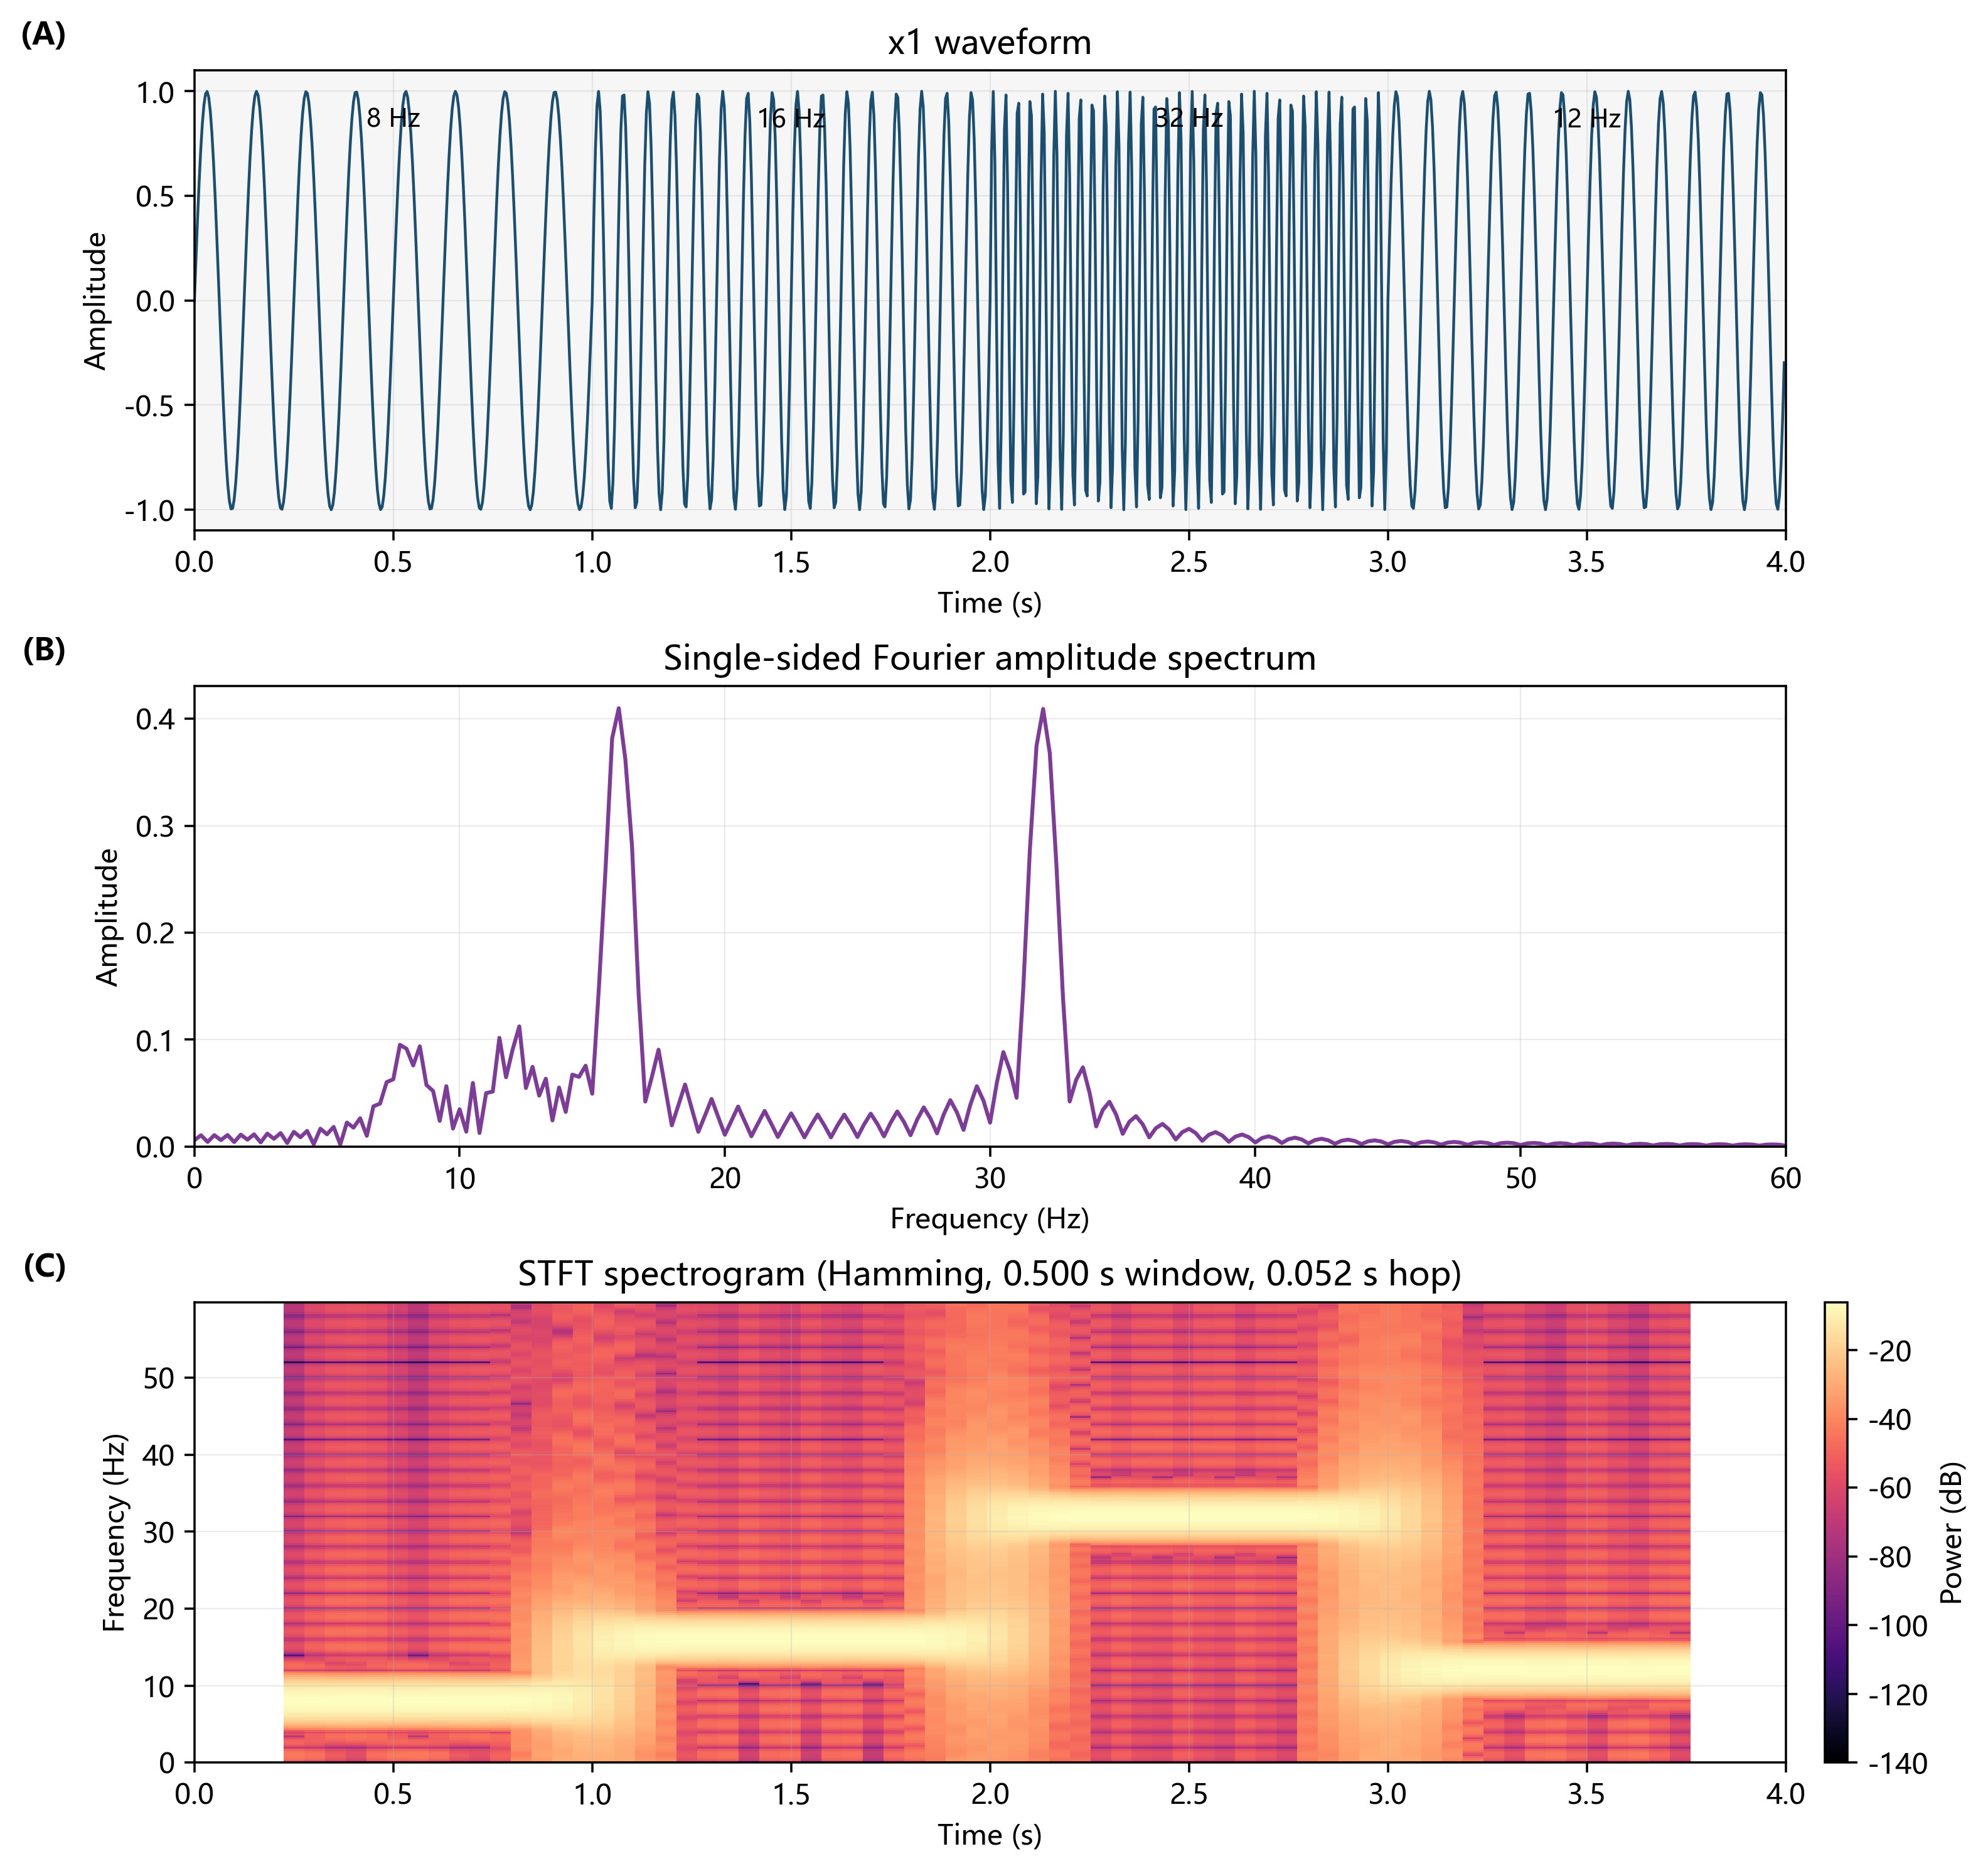
\includegraphics[width=0.96\textwidth]{exp1_x1_overview.png}
\caption{Waveform, full-record Fourier amplitude spectrum, and STFT spectrogram of the piecewise signal $x_1$. The Fourier spectrum shows multiple peaks but does not encode their occurrence times; STFT unfolds the 8, 16, 32, and 12 Hz sequence along time.}
\label{fig:exp1-x1}
\end{figure}


Figure \ref{fig:exp1-x2} compares the three views of the chirp. The waveform becomes denser over time, the full spectrum spreads over a broad frequency range, and the STFT map shows an upward high-energy ridge. The cyan curve is the analytic $f_i(t)=5+10t$ trend.

\begin{figure}[H]
\centering
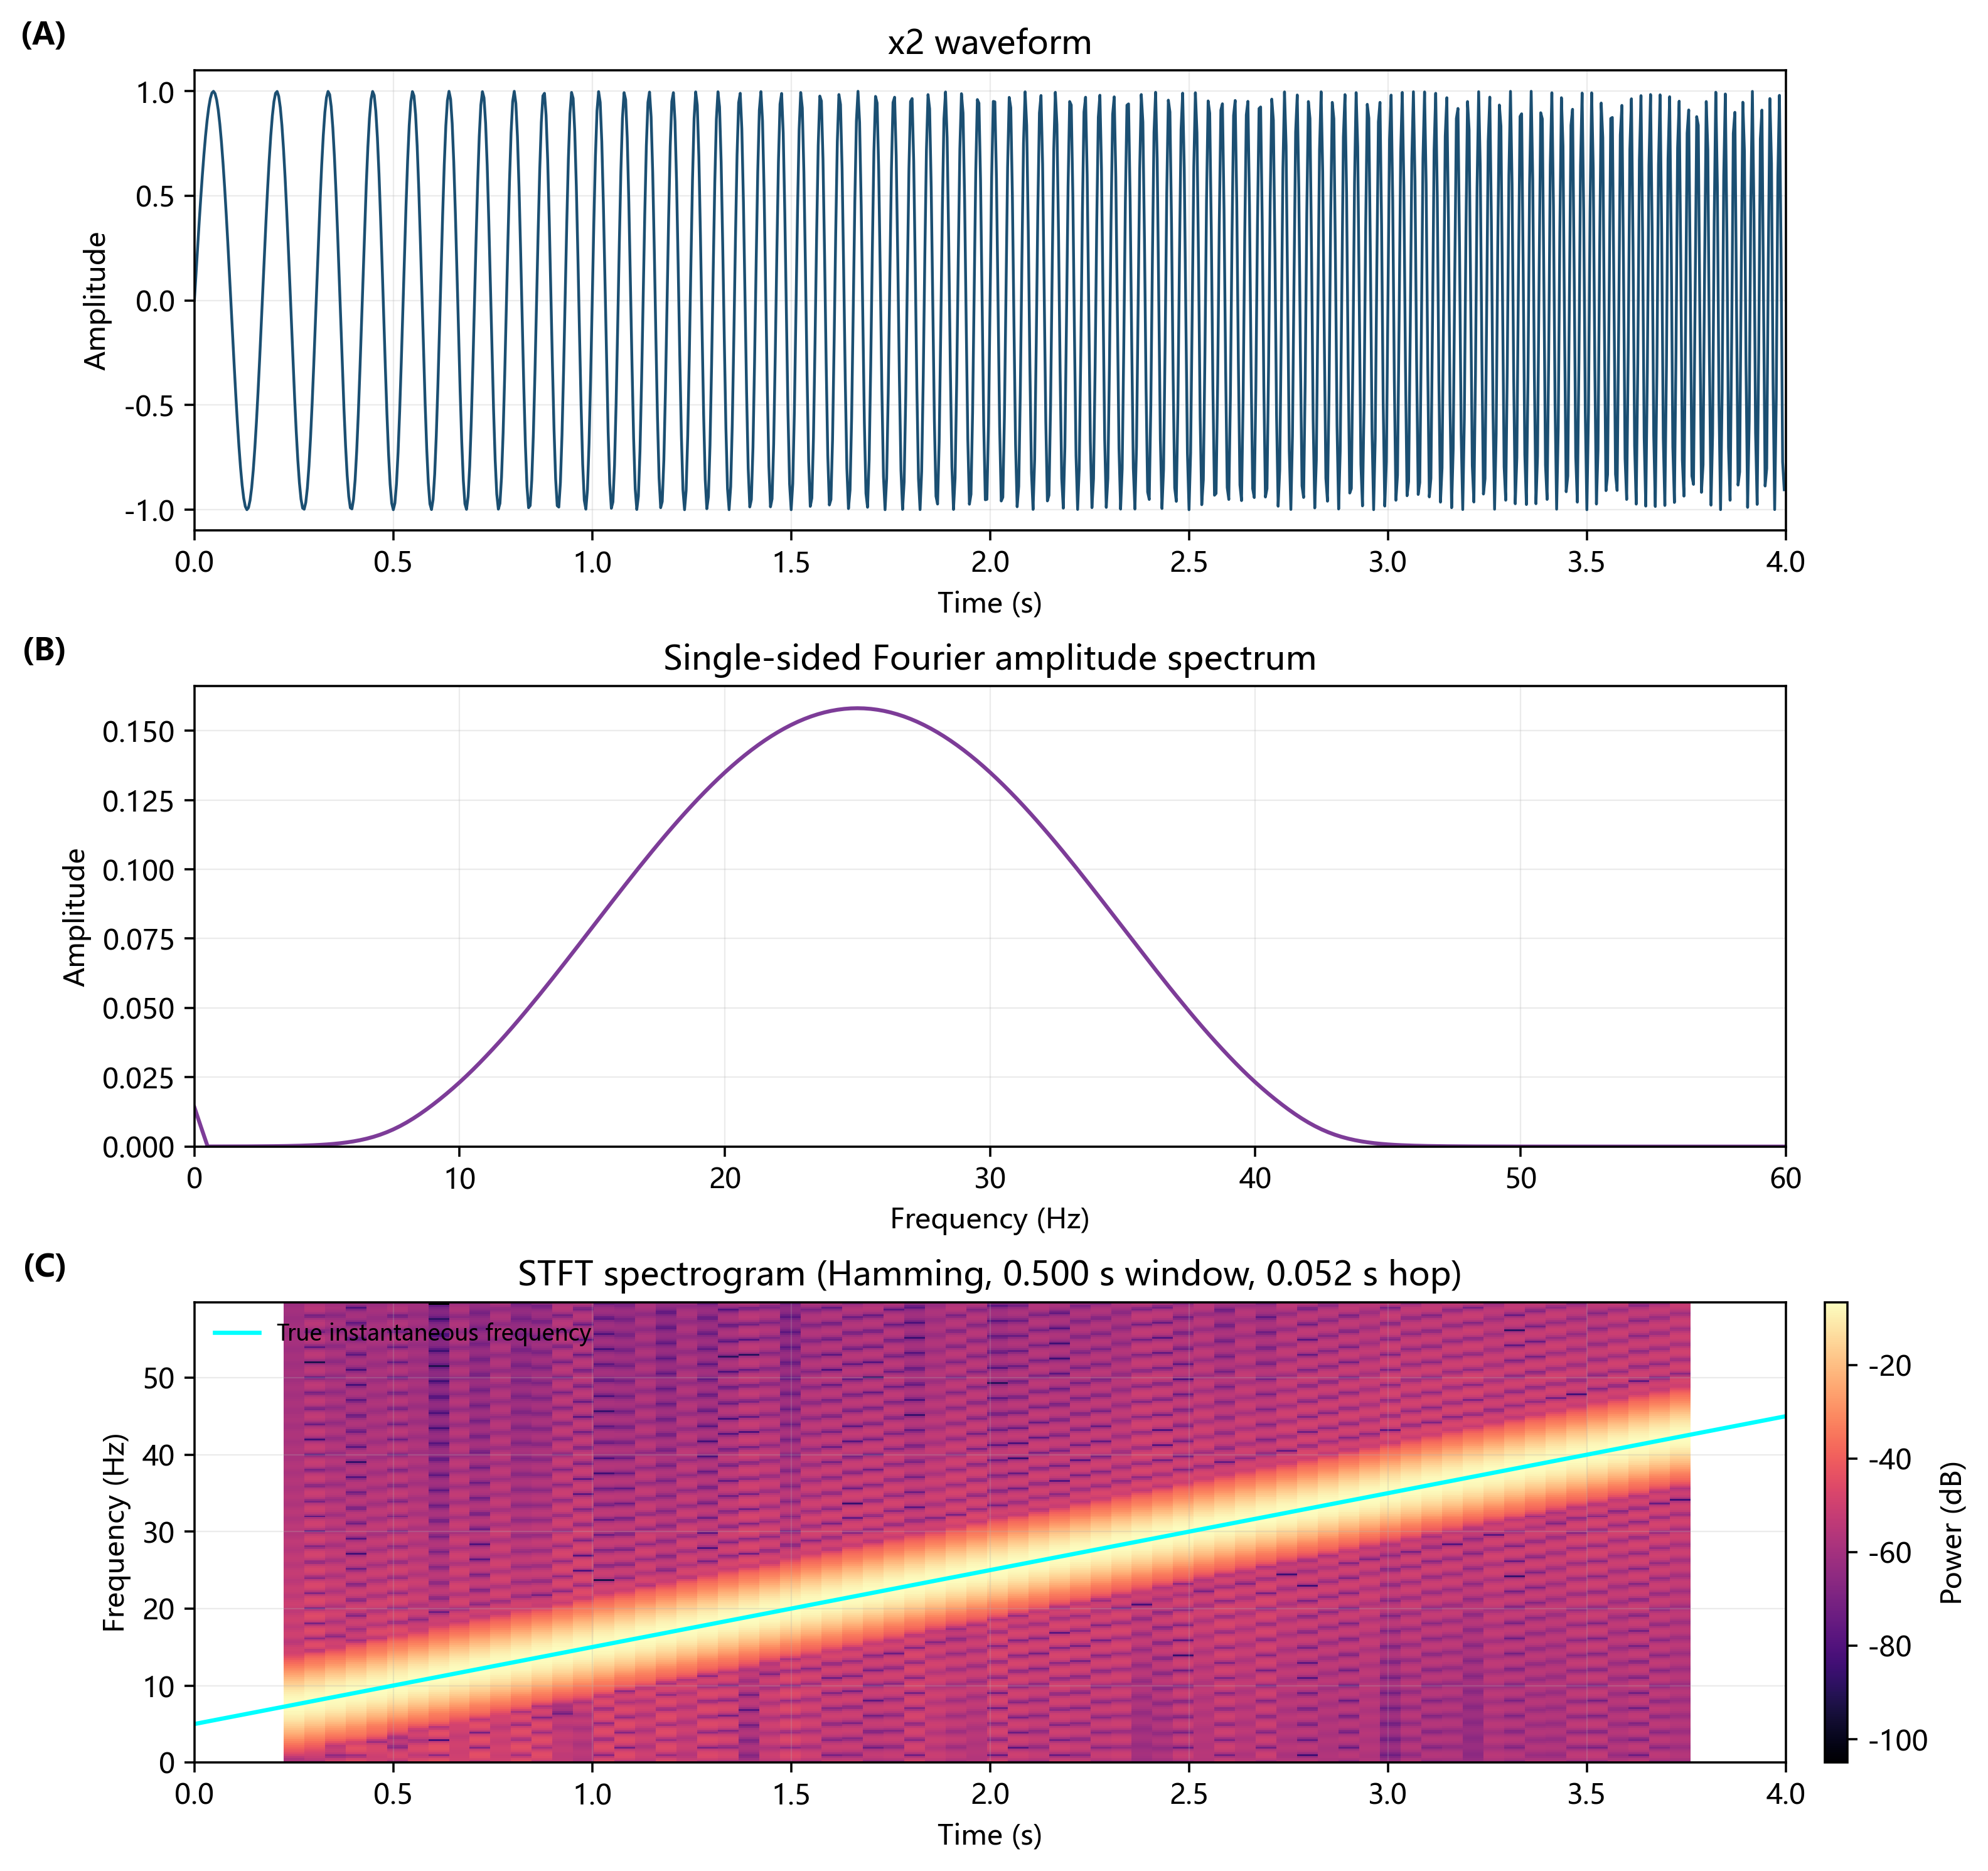
\includegraphics[width=0.96\textwidth]{exp1_x2_overview.png}
\caption{Waveform, full-record Fourier amplitude spectrum, and STFT spectrogram of the linear chirp $x_2$. The cyan curve is the true instantaneous frequency $f_i(t)=5+10t$.}
\label{fig:exp1-x2}
\end{figure}


Figure \ref{fig:exp1-ridge} extracts the ridge and compares it with the analytic trend. The MAE is 0.061 Hz and the RMSE is 0.070 Hz, indicating close tracking with residual error caused by finite window averaging and frequency-grid discretization.

\begin{figure}[H]
\centering
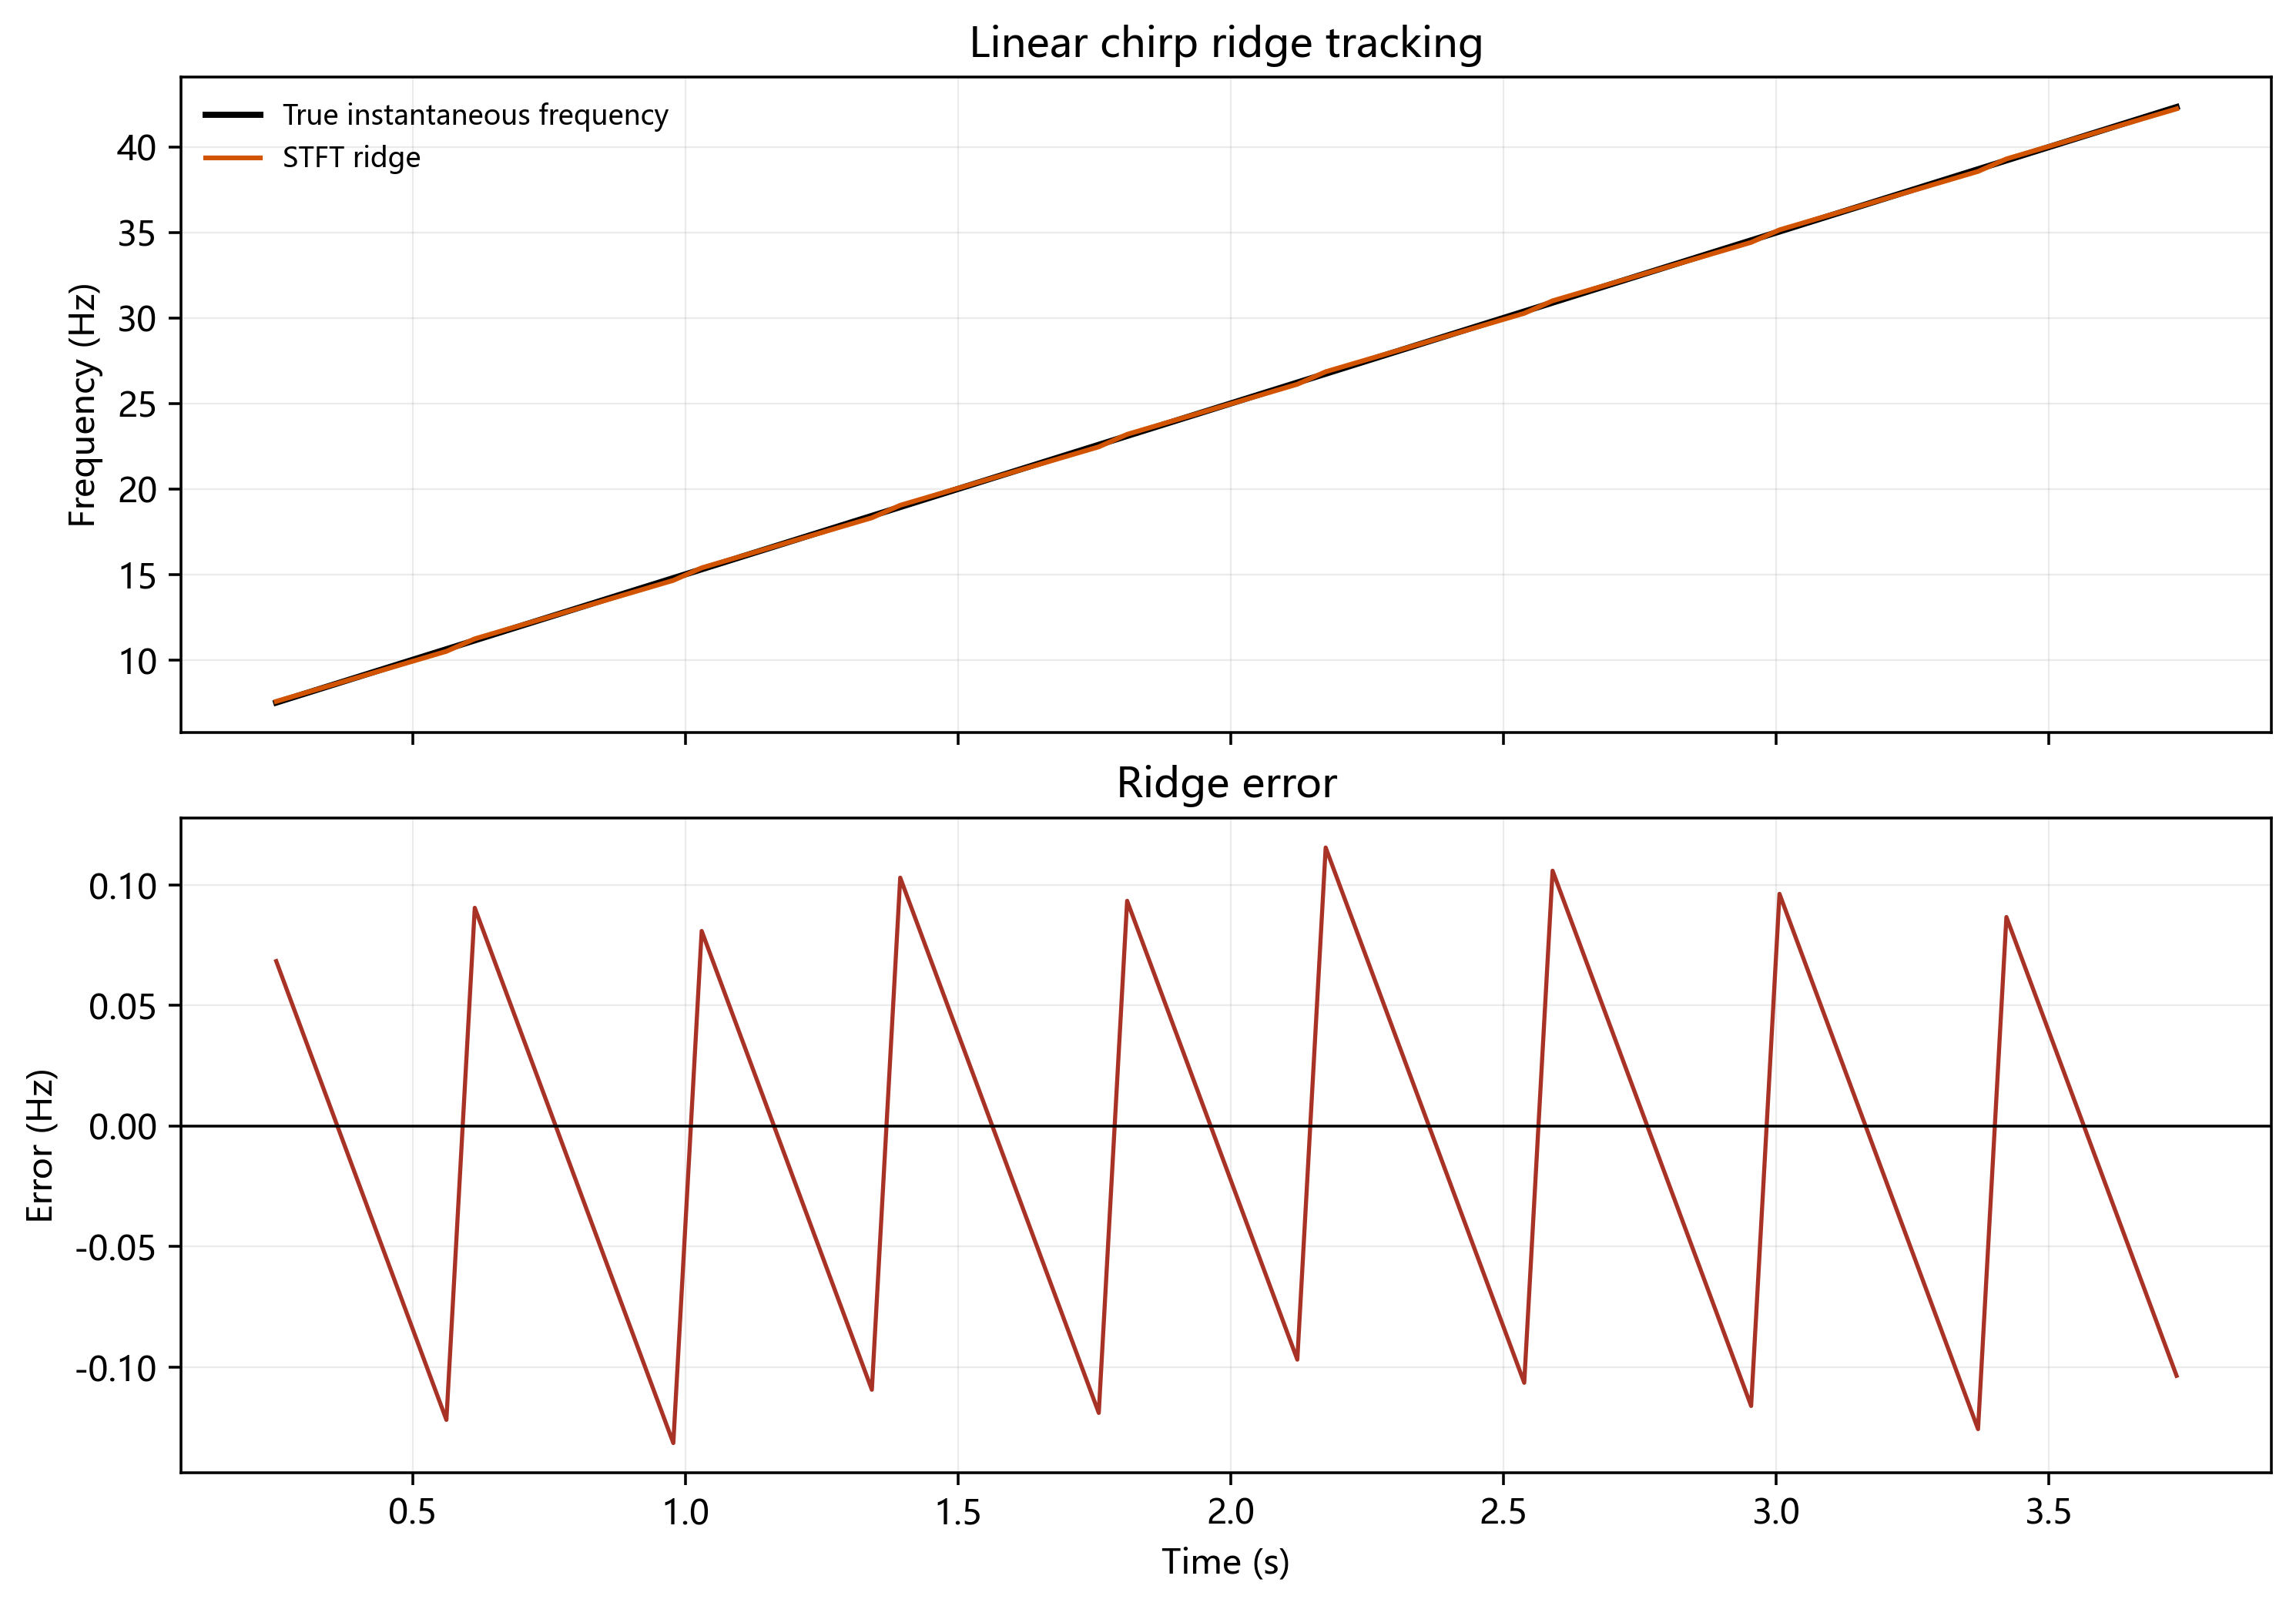
\includegraphics[width=0.96\textwidth]{exp1_chirp_ridge_error.png}
\caption{Quantitative STFT ridge check for the linear chirp. The mean absolute error is about 0.061 Hz and the root mean square error is about 0.070 Hz.}
\label{fig:exp1-ridge}
\end{figure}


Table \ref{tab:exp1-peaks} converts the visual observations into reproducible numbers. For $x_1$, the detected spectral peaks support the known frequency composition. For $x_2$, the ridge metrics quantify agreement with the analytic instantaneous frequency.

\begin{table}[H]
\centering
\caption{Main full-record Fourier peaks and chirp ridge error summary for Experiment 1.}
\label{tab:exp1-peaks}
\scriptsize
\resizebox{\textwidth}{!}{%
\begin{tabular}{llll}
\toprule
Signal & Rank & Frequency/error (Hz) & Amplitude/RMSE\\
\midrule
piecewise x1 & 1.000 & 16.000 & 0.410\\
piecewise x1 & 2.000 & 32.000 & 0.409\\
piecewise x1 & 3.000 & 12.250 & 0.112\\
piecewise x1 & 4.000 & 7.750 & 0.095\\
piecewise x1 & 5.000 & 17.500 & 0.091\\
piecewise x1 & 6.000 & 10.500 & 0.059\\
piecewise x1 & 7.000 & 30.500 & 0.088\\
piecewise x1 & 8.000 & 18.500 & 0.058\\
linear chirp x2 & 1.000 & 25.000 & 0.158\\
x2 ridge error & 1.000 & 0.061 & 0.070\\
\bottomrule
\end{tabular}
}
\end{table}


\subsection{Analysis and Discussion}
Figure \ref{fig:exp1-x1} should be read in three layers. The waveform shows four equal-amplitude sinusoids with different periods. The full Fourier spectrum shows energy near 8, 12, 16, and 32 Hz, so it verifies the frequency content. The STFT map further shows that these frequencies do not persist simultaneously; they occur in the order specified by the formula. Table \ref{tab:exp1-peaks} supports the frequency-composition claim but cannot reconstruct the timing order by itself.

Figure \ref{fig:exp1-x2} illustrates continuous frequency variation. The waveform oscillates more densely later in time, and the full spectrum becomes broad rather than a few narrow peaks. The STFT ridge follows the analytic curve $f_i(t)=5+10t$. Figure \ref{fig:exp1-ridge} gives a numerical check: MAE 0.061 Hz and RMSE 0.070 Hz. The remaining error is expected because STFT estimates local spectra over finite windows.

\paragraph{Question: Why can the full Fourier transform show multiple frequency components but not their occurrence times?}
Answer: The Fourier transform projects the entire record onto infinite-duration sinusoids. The coefficient at one frequency collects contributions from all samples, so it indicates whether that frequency exists globally, but not when it exists. For $x_1$, the 8, 16, 32, and 12 Hz components appear as spectrum peaks, but the spectrum alone cannot state which one came first.

\paragraph{Question: If only the full Fourier spectrum is observed, can we tell whether four frequencies appear sequentially or simultaneously?}
Answer: No. A sequential signal and a simultaneous mixture can have similar global spectral peaks. The phase and amplitude details may differ, but the simple amplitude spectrum does not provide a direct time-order representation. STFT resolves this ambiguity by computing local spectra over sliding windows.

\paragraph{Question: What operation does STFT add compared with the ordinary Fourier transform, and why does it provide local time information?}
Answer: STFT adds a sliding window $w(t-\tau)$. Each local spectrum mainly reflects samples near $\tau$. Moving the window center over time arranges these local spectra into a time-frequency map. This temporal localization is gained at the cost of finite time-frequency resolution.

\paragraph{Question: In real EEG, EMG, or ECG, what misunderstanding can arise if only the full spectrum is reported?}
Answer: A full spectrum may merge baseline rhythms, task-related changes, and artifacts into one global summary. A transient EMG burst, a task-related EEG ERD, or a brief ECG abnormality may appear only as a weak global peak or may be hidden by stronger background components. Timing-sensitive biomedical interpretation therefore requires time-resolved evidence.

\FloatBarrier
\clearpage
\section{Experiment 2: STFT Window Length, Window Function, and Resolution Tradeoff}
\subsection{Methods}
The signal is
\begin{equation}
x_3(t)=\sin(2\pi 10t)+0.8I_{[1.2,2.2)}(t)\sin(2\pi 12t)+1.2I_{[2.6,2.9)}(t)\sin(2\pi 35t).
\end{equation}
It contains a sustained 10 Hz component, a local 12 Hz component, and a short 35 Hz burst. Window-length comparisons use a fixed Hamming window and 0.05 s hop, with window lengths 0.25, 0.5, and 1.0 s. Window-function comparisons use a fixed 0.5 s length and 0.05 s hop with rectangular, Hann, and Hamming windows. Axes and color ranges are kept comparable within each figure group.

The 35 Hz burst is summarized by the time of maximum band energy and the half-height temporal spread. The 10--12 Hz separability is summarized by the valley ratio between two local peaks in the average 8--15 Hz profile:
\begin{equation}
R_\mathrm{valley}=1-\frac{P_\mathrm{valley}}{\min(P_{10},P_{12})} .
\end{equation}
A larger value indicates a deeper valley between the two peaks. This is an auxiliary metric; zero padding can refine display grids but cannot overcome the intrinsic resolution imposed by effective window length.

\Needspace{0.72\textheight}
\subsection{Results}
Figure \ref{fig:exp2-wave} first establishes the signal truth: the 12 Hz component occurs only from 1.2 to 2.2 s, and the 35 Hz component only from 2.6 to 2.9 s. The full spectrum shows frequency content but not local duration.

\begin{figure}[H]
\centering
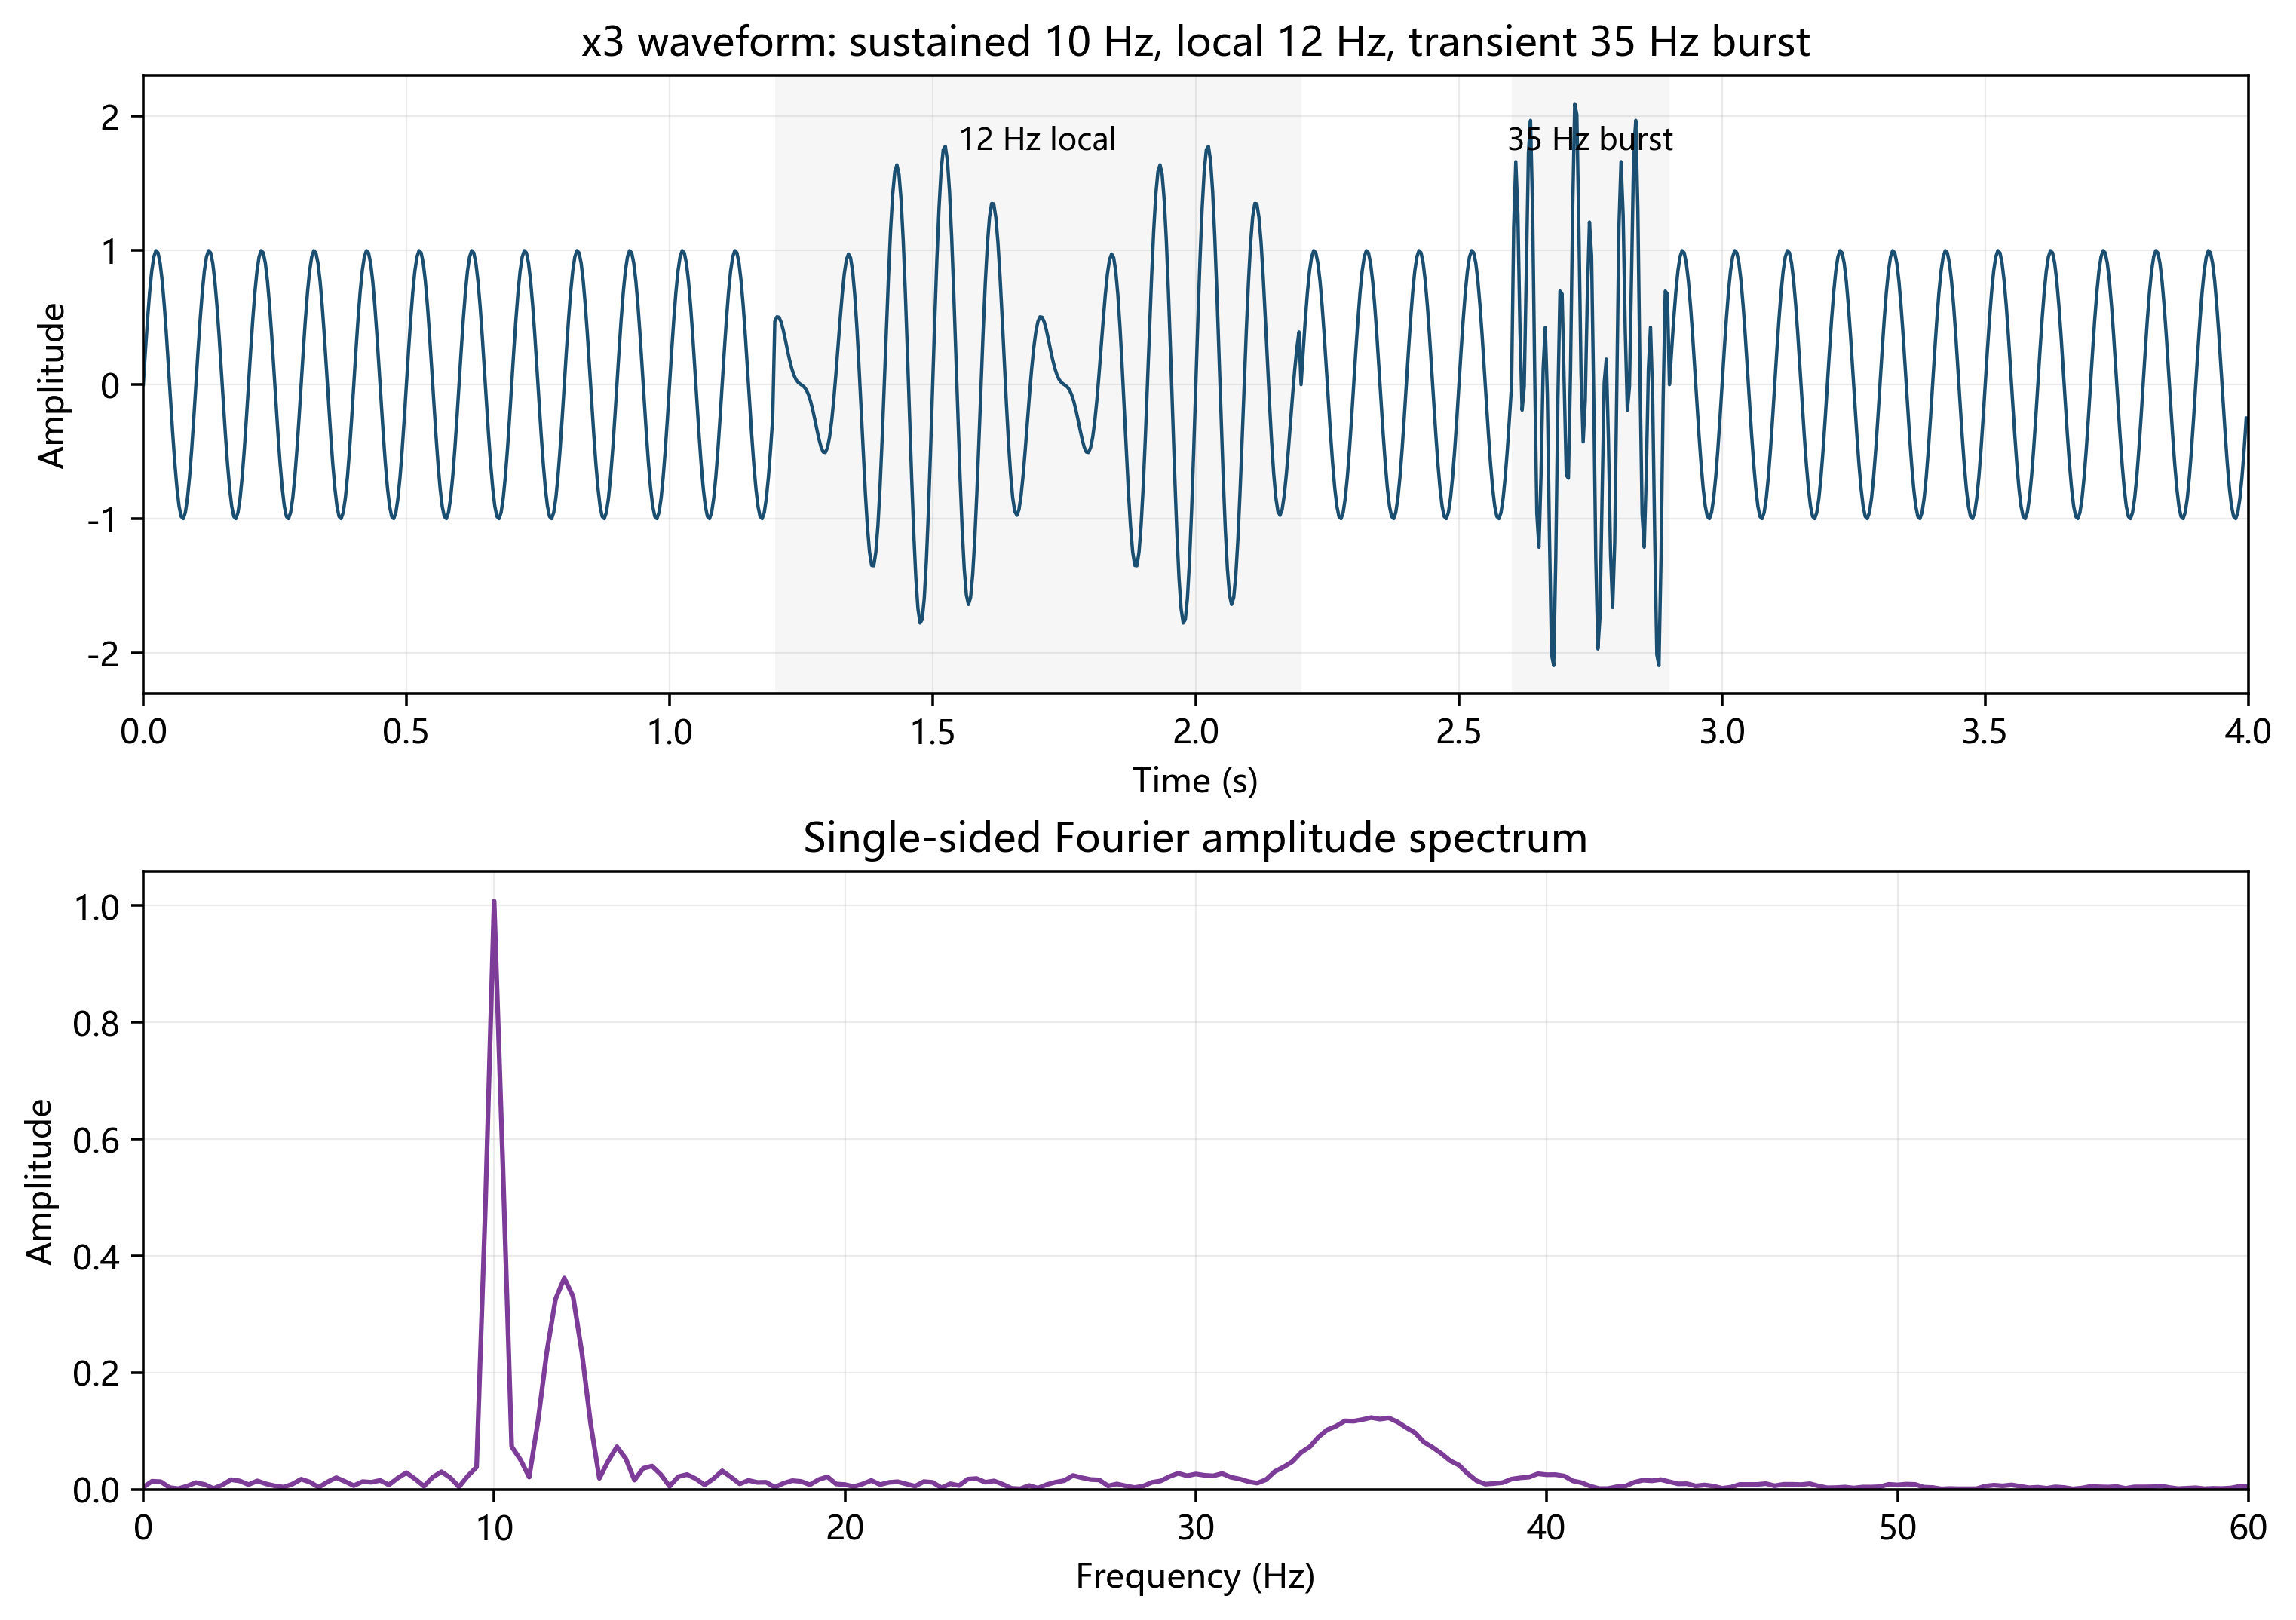
\includegraphics[width=0.96\textwidth]{exp2_x3_wave_fft.png}
\caption{Waveform and full-record Fourier spectrum of $x_3$. The 12 Hz component is local to 1.2--2.2 s and the 35 Hz component is a short 2.6--2.9 s burst.}
\label{fig:exp2-wave}
\end{figure}


Figure \ref{fig:exp2-lengths} compares three window lengths. The short window localizes the 35 Hz burst more tightly, while the long window stabilizes low-frequency ridges and spreads the high-frequency burst in time.

\begin{figure}[H]
\centering
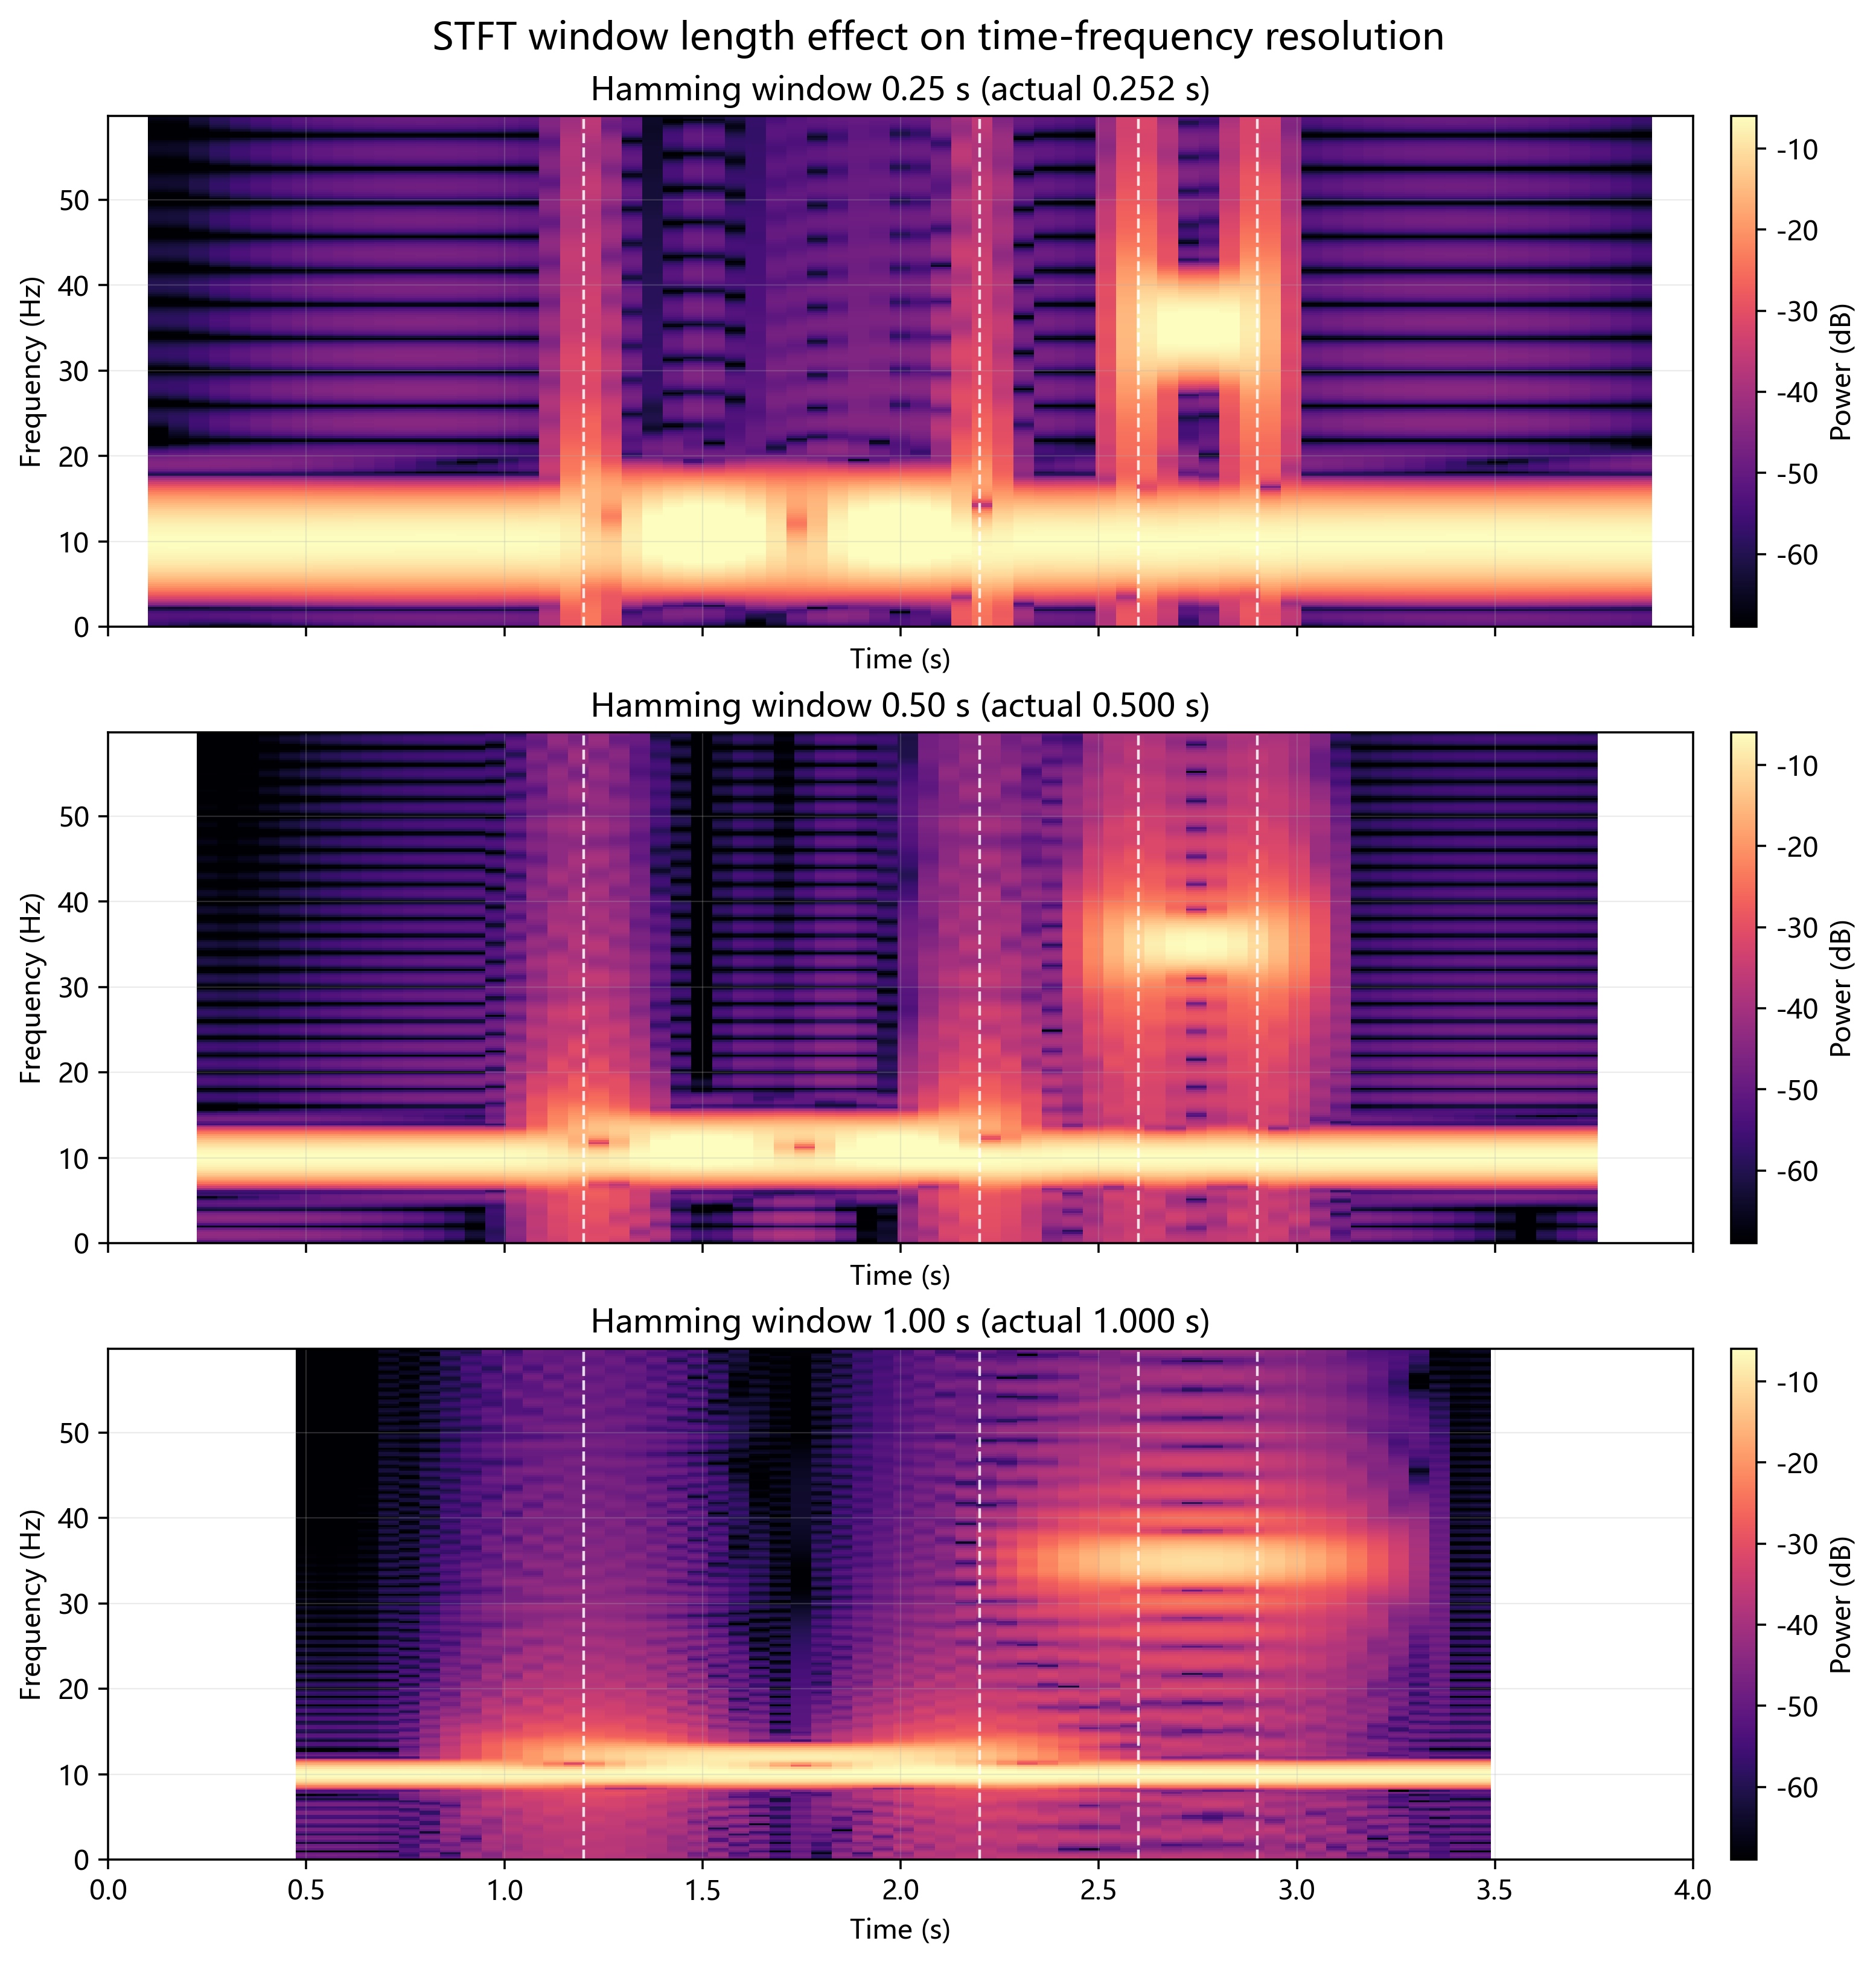
\includegraphics[width=0.96\textwidth]{exp2_window_lengths.png}
\caption{Effect of STFT window length. A short window improves the temporal localization of the 35 Hz burst; a long window sharpens low-frequency structure but broadens the burst in time.}
\label{fig:exp2-lengths}
\end{figure}


Figure \ref{fig:exp2-functions} shows that the window function also changes the map. The rectangular window has a narrow main lobe but high sidelobes, while Hann and Hamming taper the endpoints and reduce leakage at the cost of a broader effective main lobe.

\begin{figure}[H]
\centering
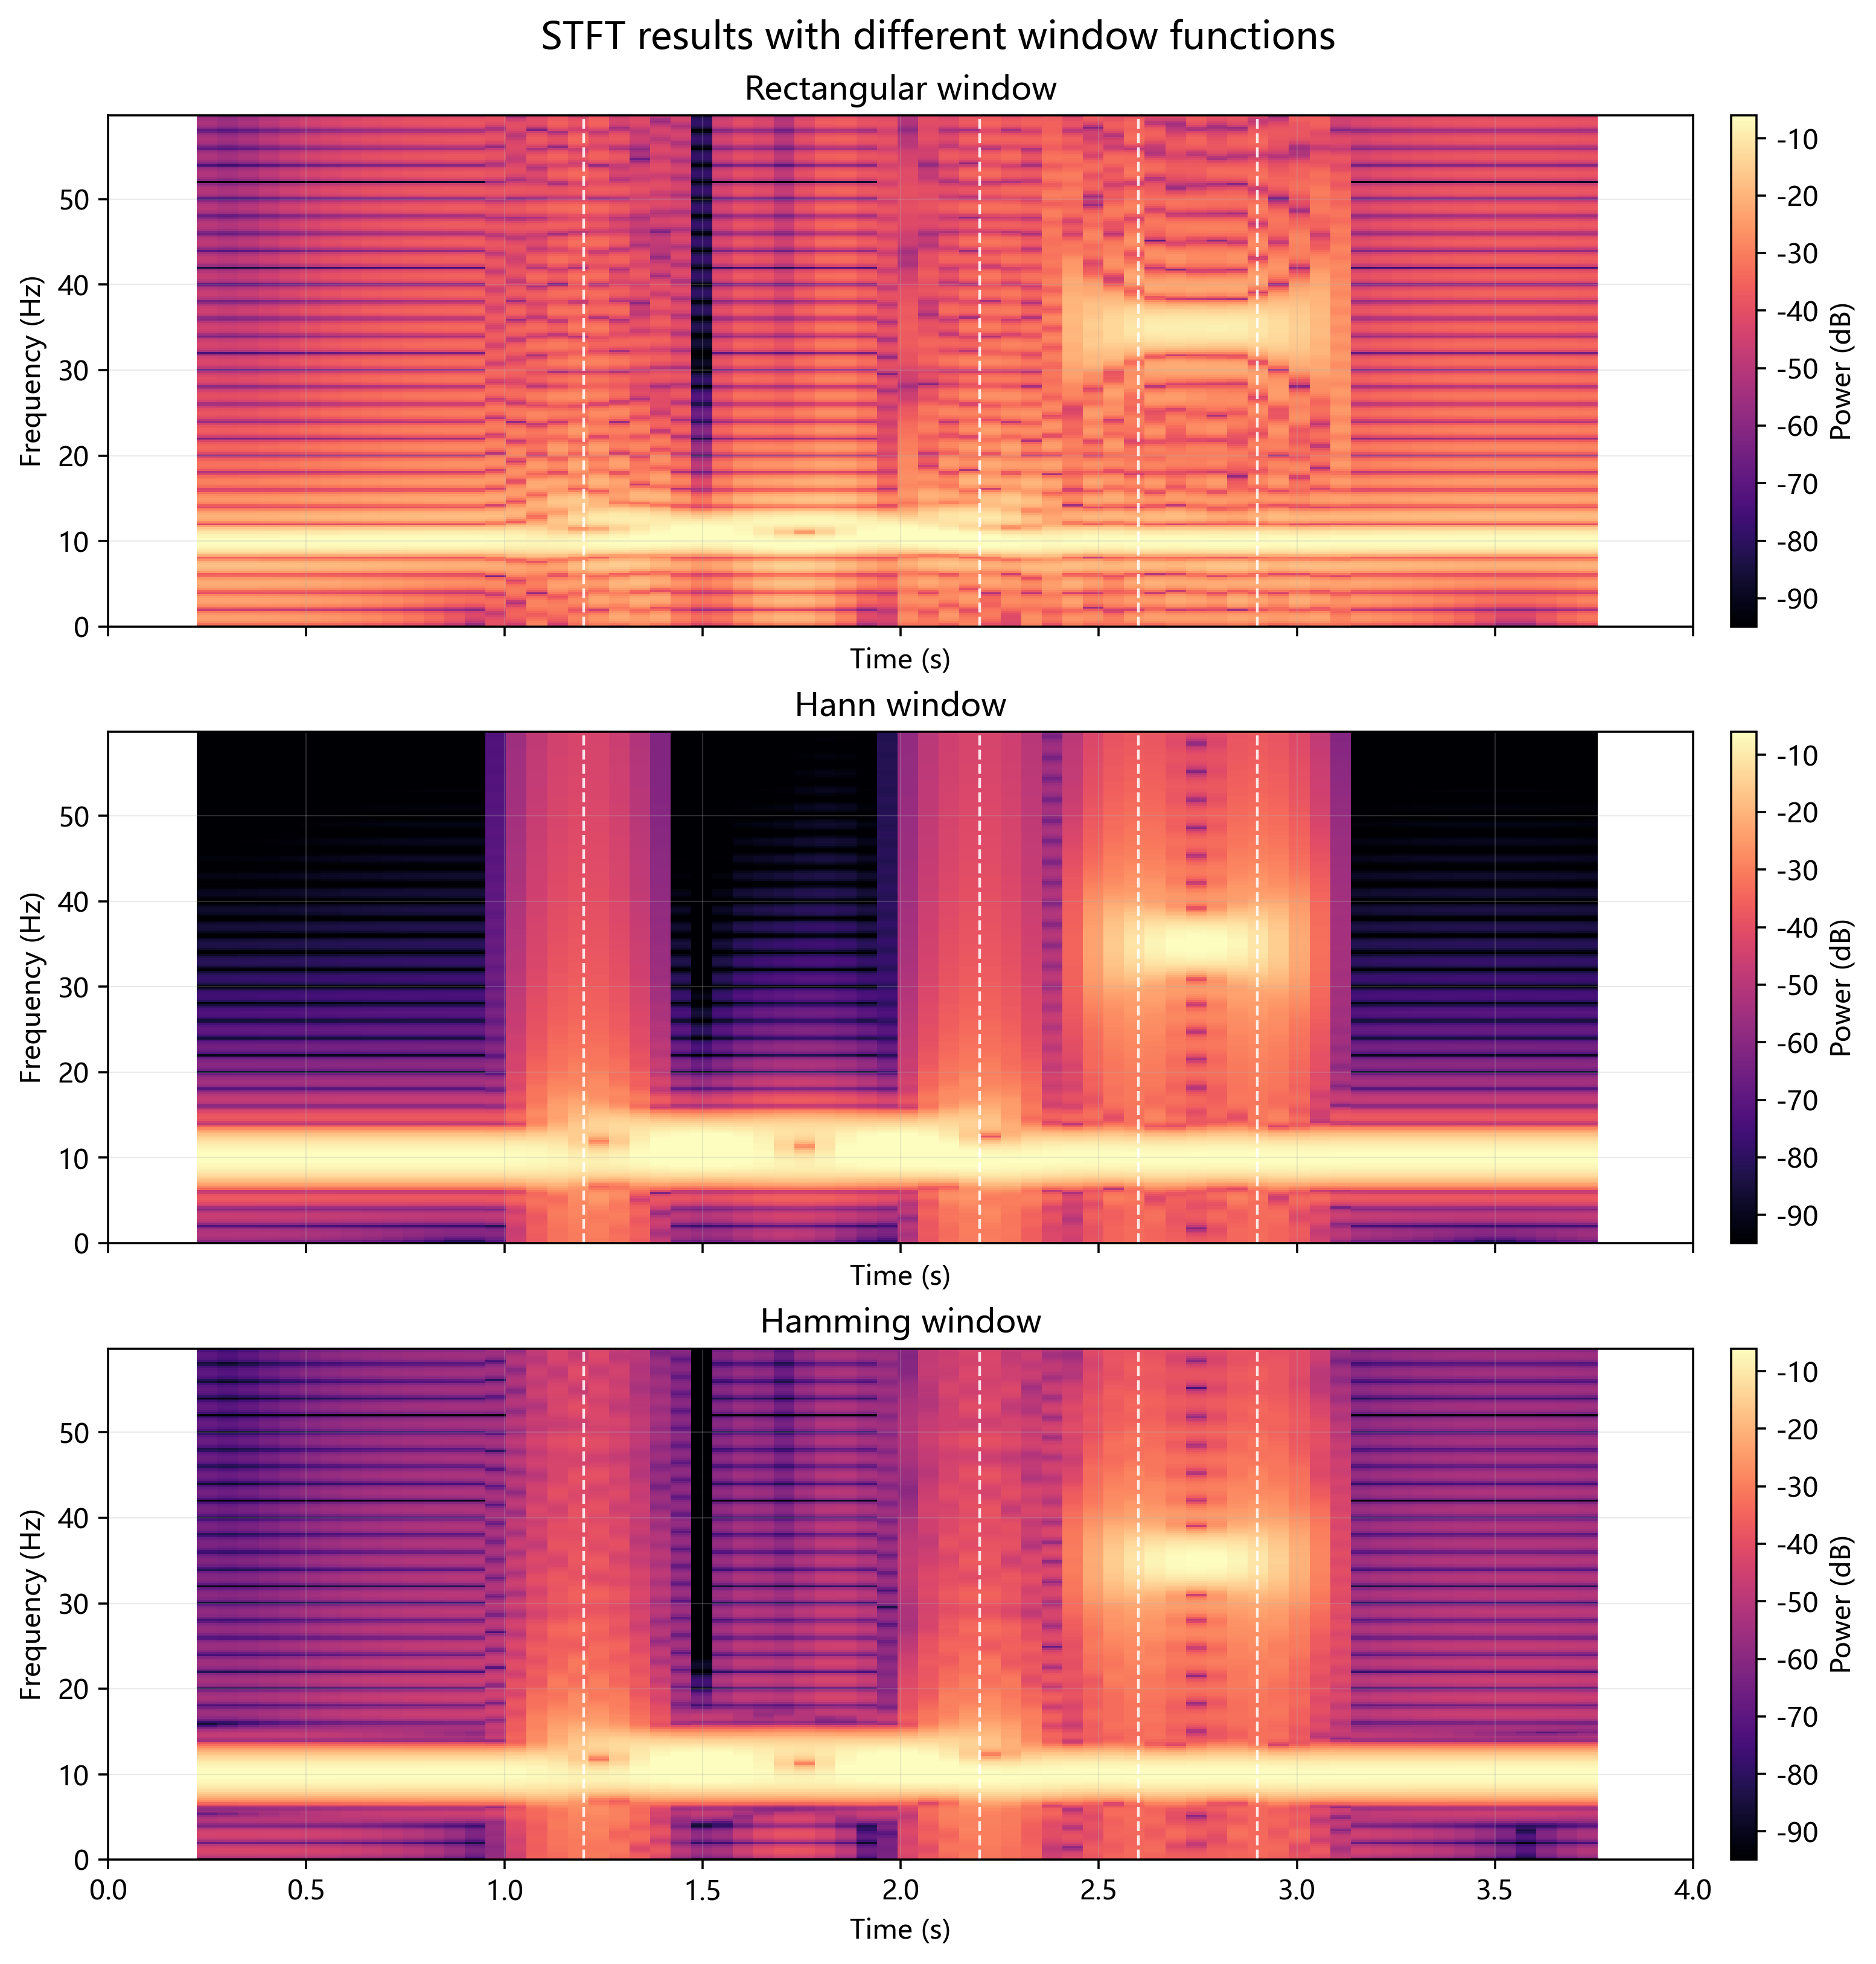
\includegraphics[width=0.96\textwidth]{exp2_window_functions.png}
\caption{Effect of window function under the same 0.5 s window length. Rectangular, Hann, and Hamming windows distribute energy differently because their sidelobe and main-lobe properties differ.}
\label{fig:exp2-functions}
\end{figure}


Figure \ref{fig:exp2-profiles} compresses the low-frequency region into average spectral profiles. A deeper valley between the 10 and 12 Hz peaks indicates better separability; a single broad peak indicates that the two nearby components are blended by the window response.

\begin{figure}[H]
\centering
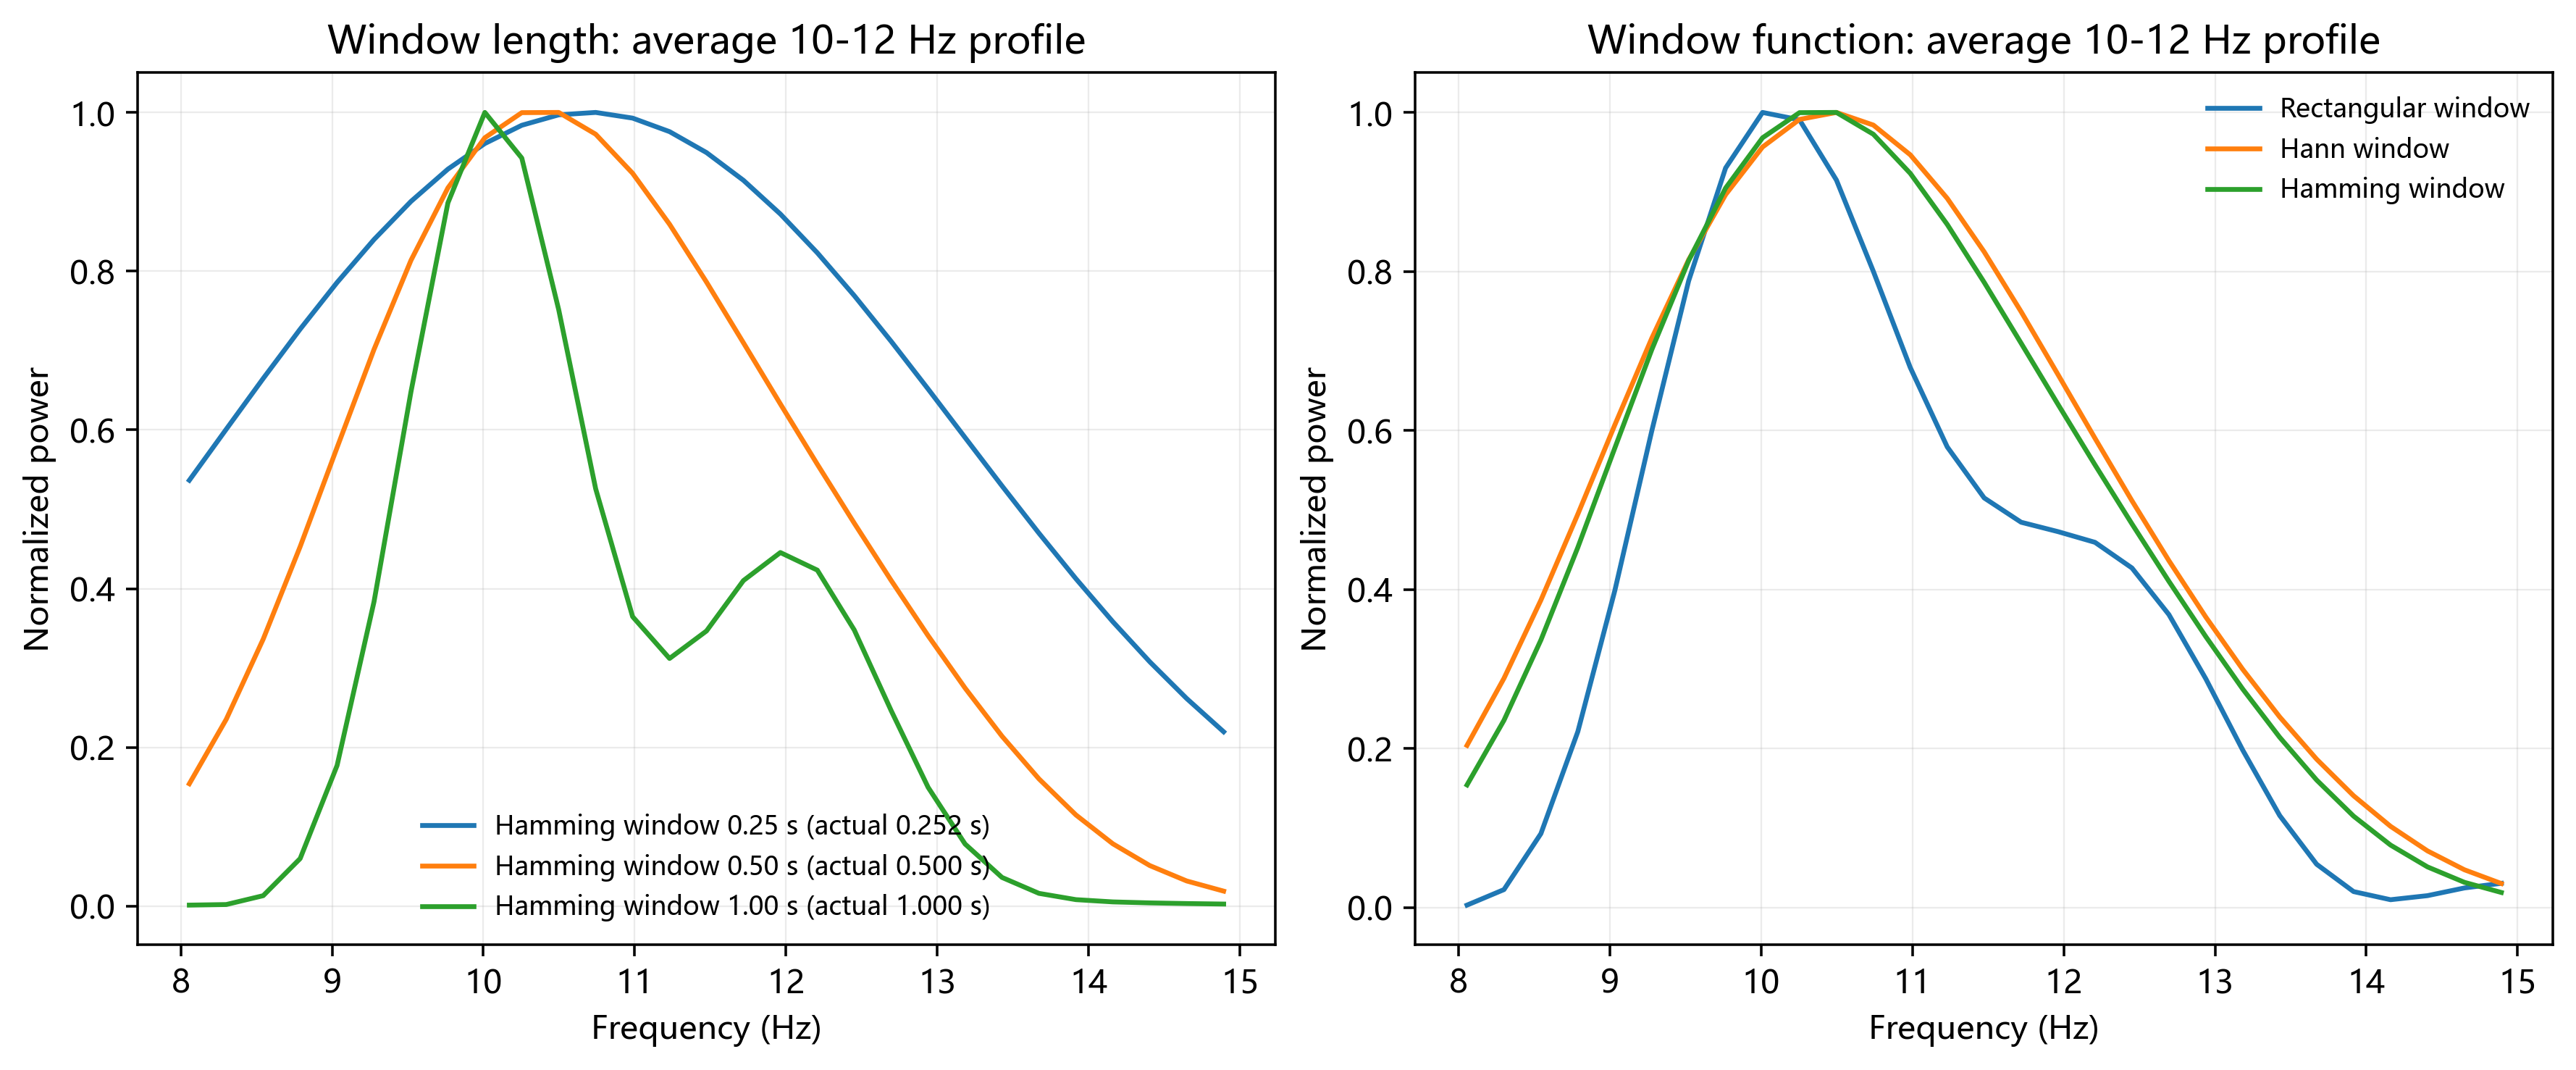
\includegraphics[width=0.96\textwidth]{exp2_low_band_profiles.png}
\caption{Average 10--12 Hz spectral profiles. The profiles complement the heatmaps by directly showing whether nearby low-frequency peaks are separated.}
\label{fig:exp2-profiles}
\end{figure}


Figure \ref{fig:exp2-explore} explicitly links parameter choice to analysis goals. A short-window setting is preferred for localizing the 35 Hz burst, while a long-window setting is preferred for distinguishing 10 and 12 Hz activity.

\begin{figure}[H]
\centering
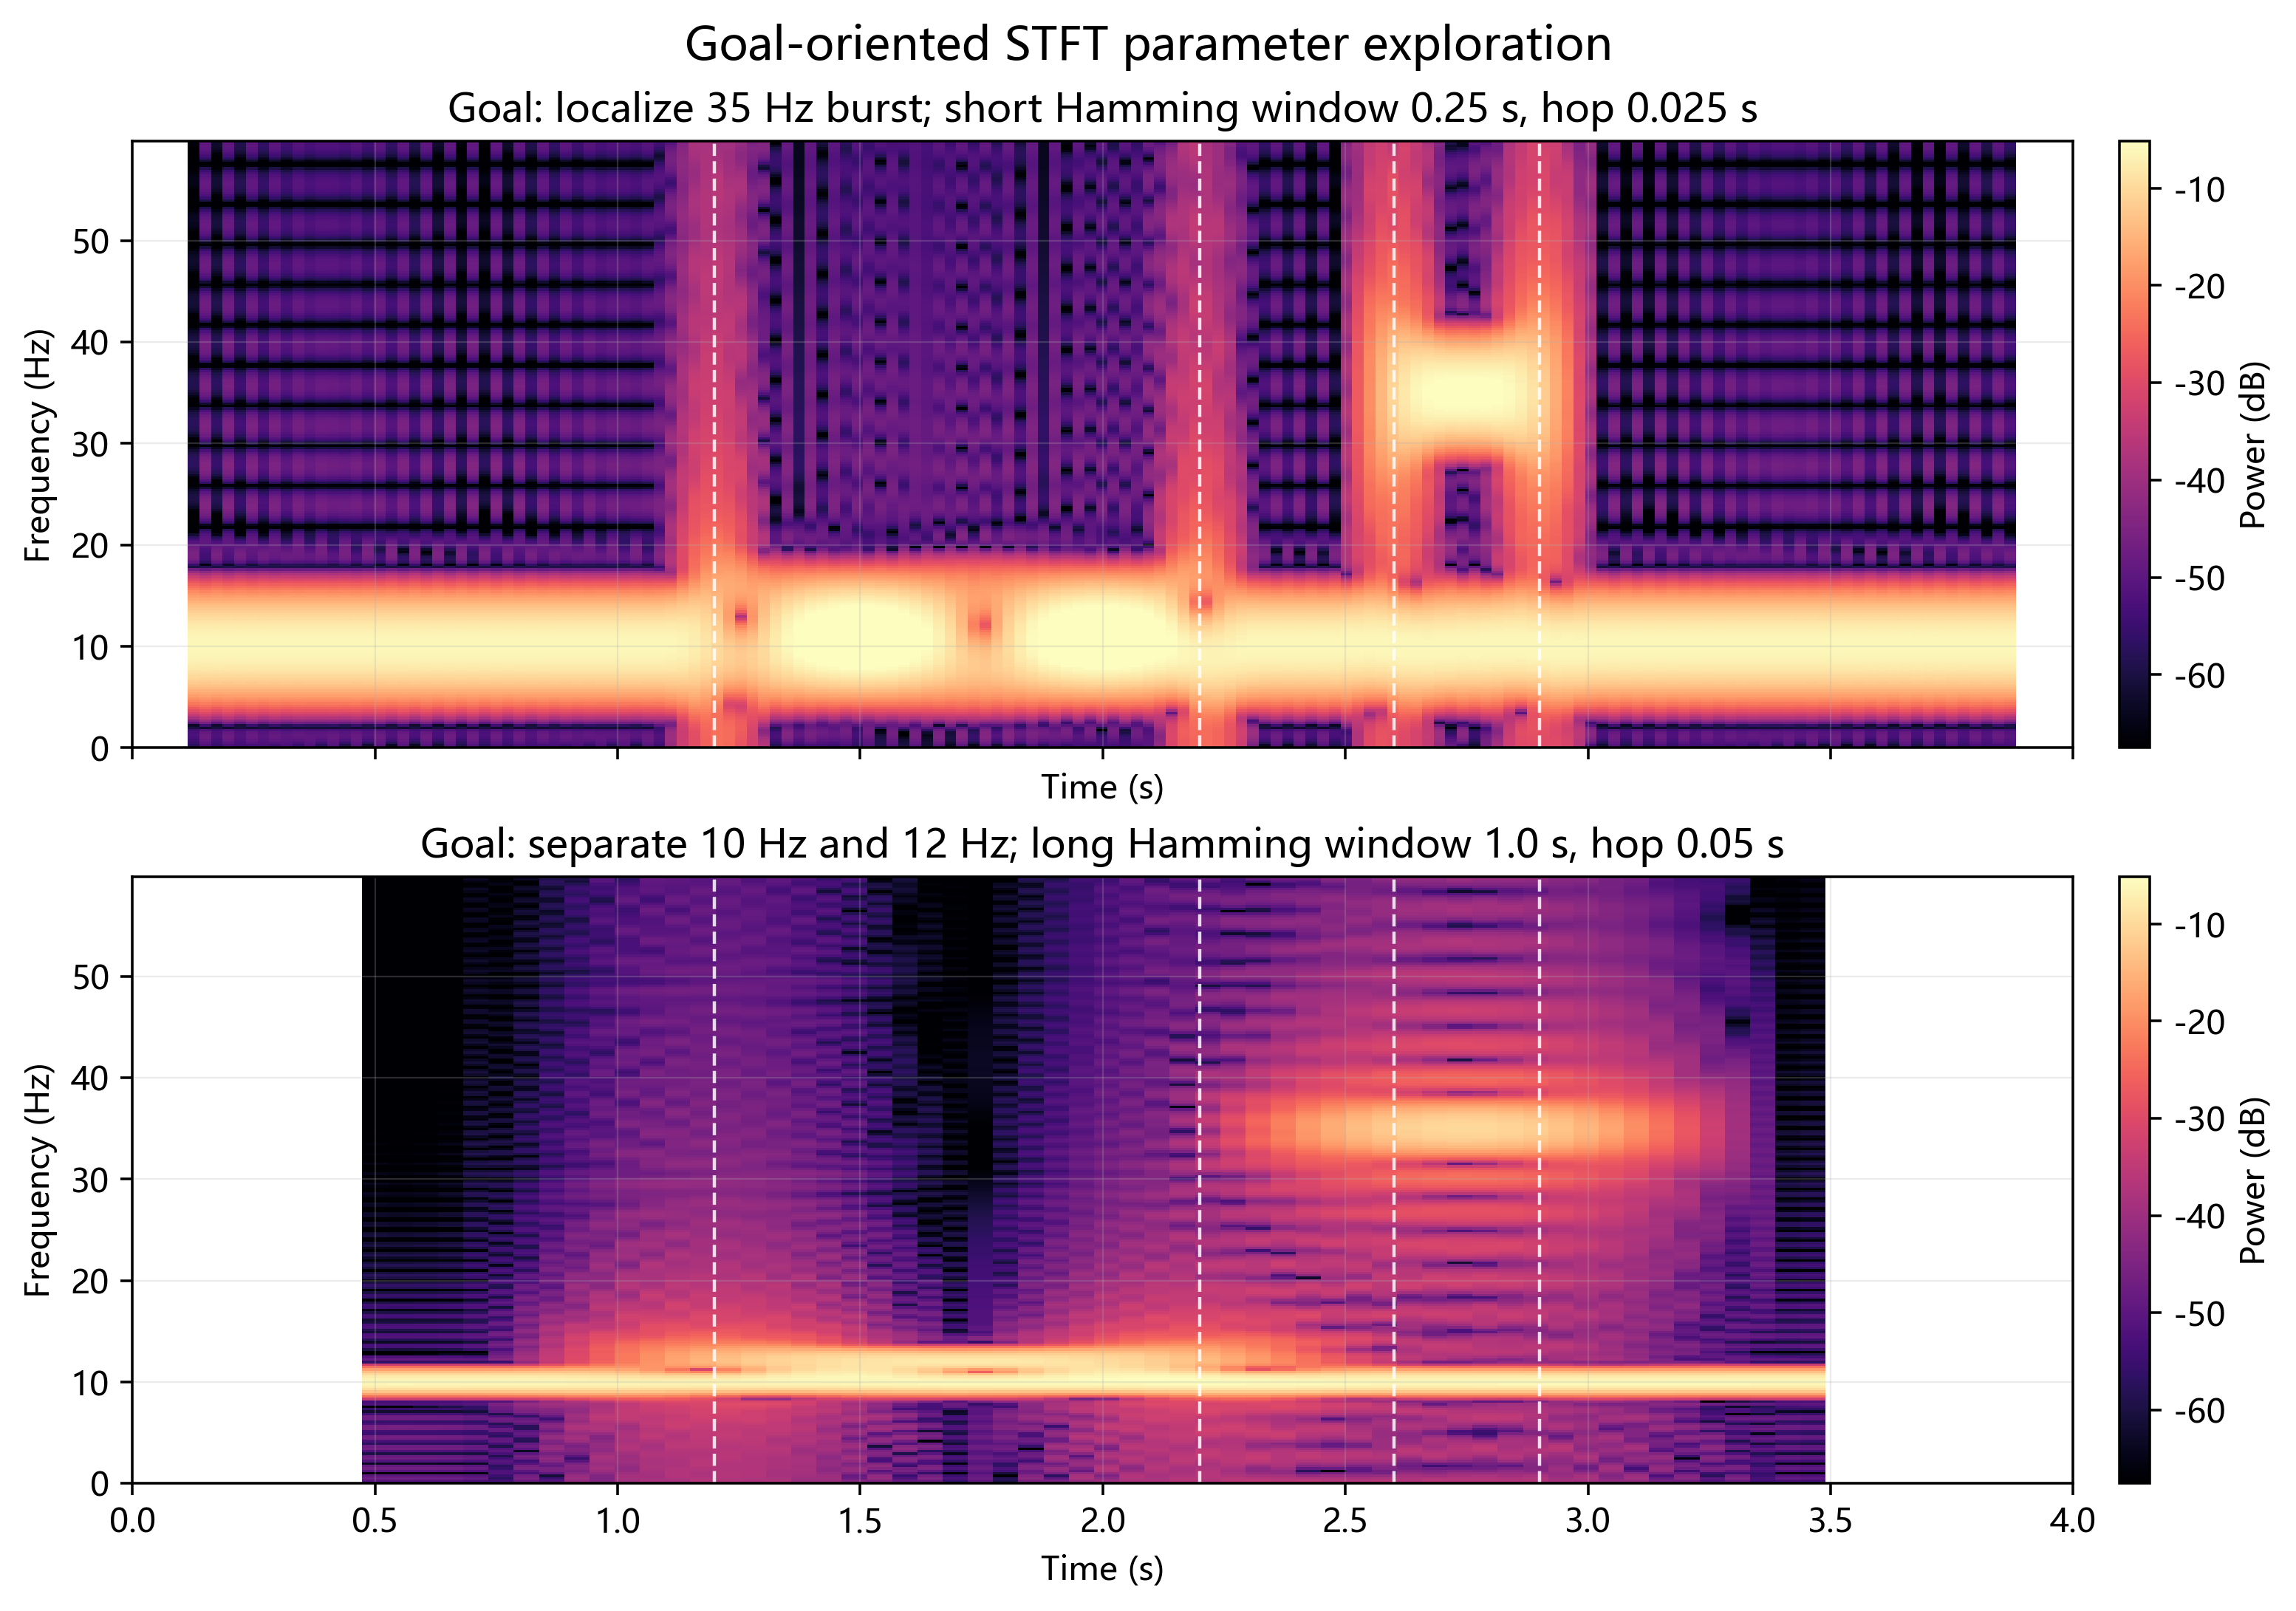
\includegraphics[width=0.96\textwidth]{exp2_parameter_exploration.png}
\caption{Goal-oriented STFT parameter exploration. Short windows favor transient localization; long windows favor nearby low-frequency separation.}
\label{fig:exp2-explore}
\end{figure}


Table \ref{tab:exp2-metrics} reports the half-height spread and valley ratio. The short-window 35 Hz spread is 0.156 s, whereas the long-window spread is 0.364 s. The low-frequency valley ratio changes from 0.000 to 0.300, matching the visual tradeoff.

\begin{table}[H]
\centering
\caption{Semi-quantitative STFT parameter metrics for Experiment 2.}
\label{tab:exp2-metrics}
\scriptsize
\resizebox{\textwidth}{!}{%
\begin{tabular}{llllllll}
\toprule
Comparison & Setting & Actual window(s) & Actual hop(s) & 35Hz peak(s) & Half-height width(s) & Valley & 10/12 separated\\
\midrule
window length & 0.25s & 0.252 & 0.052 & 2.726 & 0.156 & 0.000 & weak/no\\
window length & 0.50s & 0.500 & 0.052 & 2.746 & 0.208 & 0.000 & weak/no\\
window length & 1.00s & 1.000 & 0.052 & 2.736 & 0.364 & 0.300 & yes\\
window function & boxcar & 0.500 & 0.052 & 2.798 & 0.416 & 0.000 & weak/no\\
window function & hann & 0.500 & 0.052 & 2.746 & 0.208 & 0.000 & weak/no\\
window function & hamming & 0.500 & 0.052 & 2.746 & 0.208 & 0.000 & weak/no\\
\bottomrule
\end{tabular}
}
\end{table}


\subsection{Analysis and Discussion}
The signal $x_3$ is designed to force a tradeoff. The 10 and 12 Hz components are only 2 Hz apart, so they require frequency resolution. The 35 Hz burst lasts only 0.3 s, so it requires temporal resolution. Figure \ref{fig:exp2-lengths} and Table \ref{tab:exp2-metrics} show that one STFT setting cannot optimize both goals simultaneously.

\paragraph{Question: Why does a short window localize a transient better but separate 10 and 12 Hz worse?}
Answer: A short window changes quickly when the burst enters or leaves the window, so temporal localization is good. However, at 10 Hz a 0.25 s window contains only about 2.5 cycles. The frequency main lobe is broad, so 10 and 12 Hz are easily merged.

\paragraph{Question: Why does a long window separate nearby frequencies better but blur the 35 Hz burst in time?}
Answer: A long window contains more cycles and narrows the spectral peak. A 1.0 s window contains about 10 cycles at 10 Hz and 12 cycles at 12 Hz. But the 35 Hz burst is only 0.3 s long; many window positions before and after the burst still include part of it, which spreads its energy over a longer time interval.

\paragraph{Question: How do rectangular, Hann, and Hamming windows differ, and why is the window not merely a display parameter?}
Answer: The rectangular window abruptly truncates the signal and therefore has higher sidelobes. Hann and Hamming windows taper endpoints and suppress leakage, but broaden the effective main lobe. Since these changes alter where energy appears in the map, the window is part of the estimator, not just a plotting style.

\paragraph{Question: How should window length be chosen for transient high-frequency bursts or nearby low-frequency rhythms?}
Answer: For short high-frequency bursts, use a relatively short window and small hop, with a window not much longer than the target event. For nearby low-frequency rhythms, use a longer window containing multiple low-frequency cycles. The choice must follow the scientific target.

\paragraph{Question: Why is ``clearer-looking'' not the same as ``more correct''?}
Answer: A visually smooth map may hide transients or exaggerate duration. A sharp-looking map may have poor frequency resolution or leakage. Correctness should be judged against the analysis goal, theoretical constraints, and quantitative metrics rather than visual clarity alone.

\FloatBarrier
\clearpage
\section{Experiment 3: Continuous Wavelet Transform and Multiscale Comparison}
\subsection{Methods}
The STFT/CWT comparison signal is
\begin{equation}
x_4(t)=\sin(2\pi 6t)+0.8I_{[1.0,2.5)}(t)\sin(2\pi 14t)+1.2I_{[3.0,3.25)}(t)\sin(2\pi 45t).
\end{equation}
The short-window STFT uses a 0.25 s Hamming window; the long-window STFT uses a 1.0 s Hamming window. CWT uses the Morlet-like complex wavelet \texttt{cmor1.5-1.0} over 2--60 Hz.

The multiresolution signal is
\begin{equation}
x_\mathrm{MRA}(t)=0.5\sin(2\pi t)+0.8\sin(2\pi 6t)+0.6\sin(2\pi 12t)+I_{[2.4,2.8)}(t)\sin(2\pi 45t).
\end{equation}
The formula contains the middle component at 12 Hz. If task wording mentions a 142 Hz middle component, this report follows the formula and interprets the component as 12 Hz.

The 45 Hz burst is summarized by peak time and half-height spread, while 6 Hz continuity is summarized by the fraction of the normalized low-frequency curve exceeding a threshold and by curve coefficient of variation. DWT uses \texttt{sym6} with six decomposition levels. The dyadic interpretation is
\begin{equation}
D_2\approx[31.25,62.5]\ \mathrm{Hz},\quad
D_4\approx[7.81,15.63]\ \mathrm{Hz},\quad
D_5\approx[3.91,7.81]\ \mathrm{Hz},\quad
A_6\approx[0,1.95]\ \mathrm{Hz}.
\end{equation}

\Needspace{0.72\textheight}
\subsection{Results}
Figure \ref{fig:exp3-compare} compares short-window STFT, long-window STFT, and CWT. The short STFT localizes the 45 Hz burst but broadens low-frequency structure. The long STFT stabilizes 6 and 14 Hz components but broadens the burst. CWT uses different scales at different frequencies, preserving a continuous low-frequency band and a relatively localized high-frequency burst.

\begin{figure}[H]
\centering
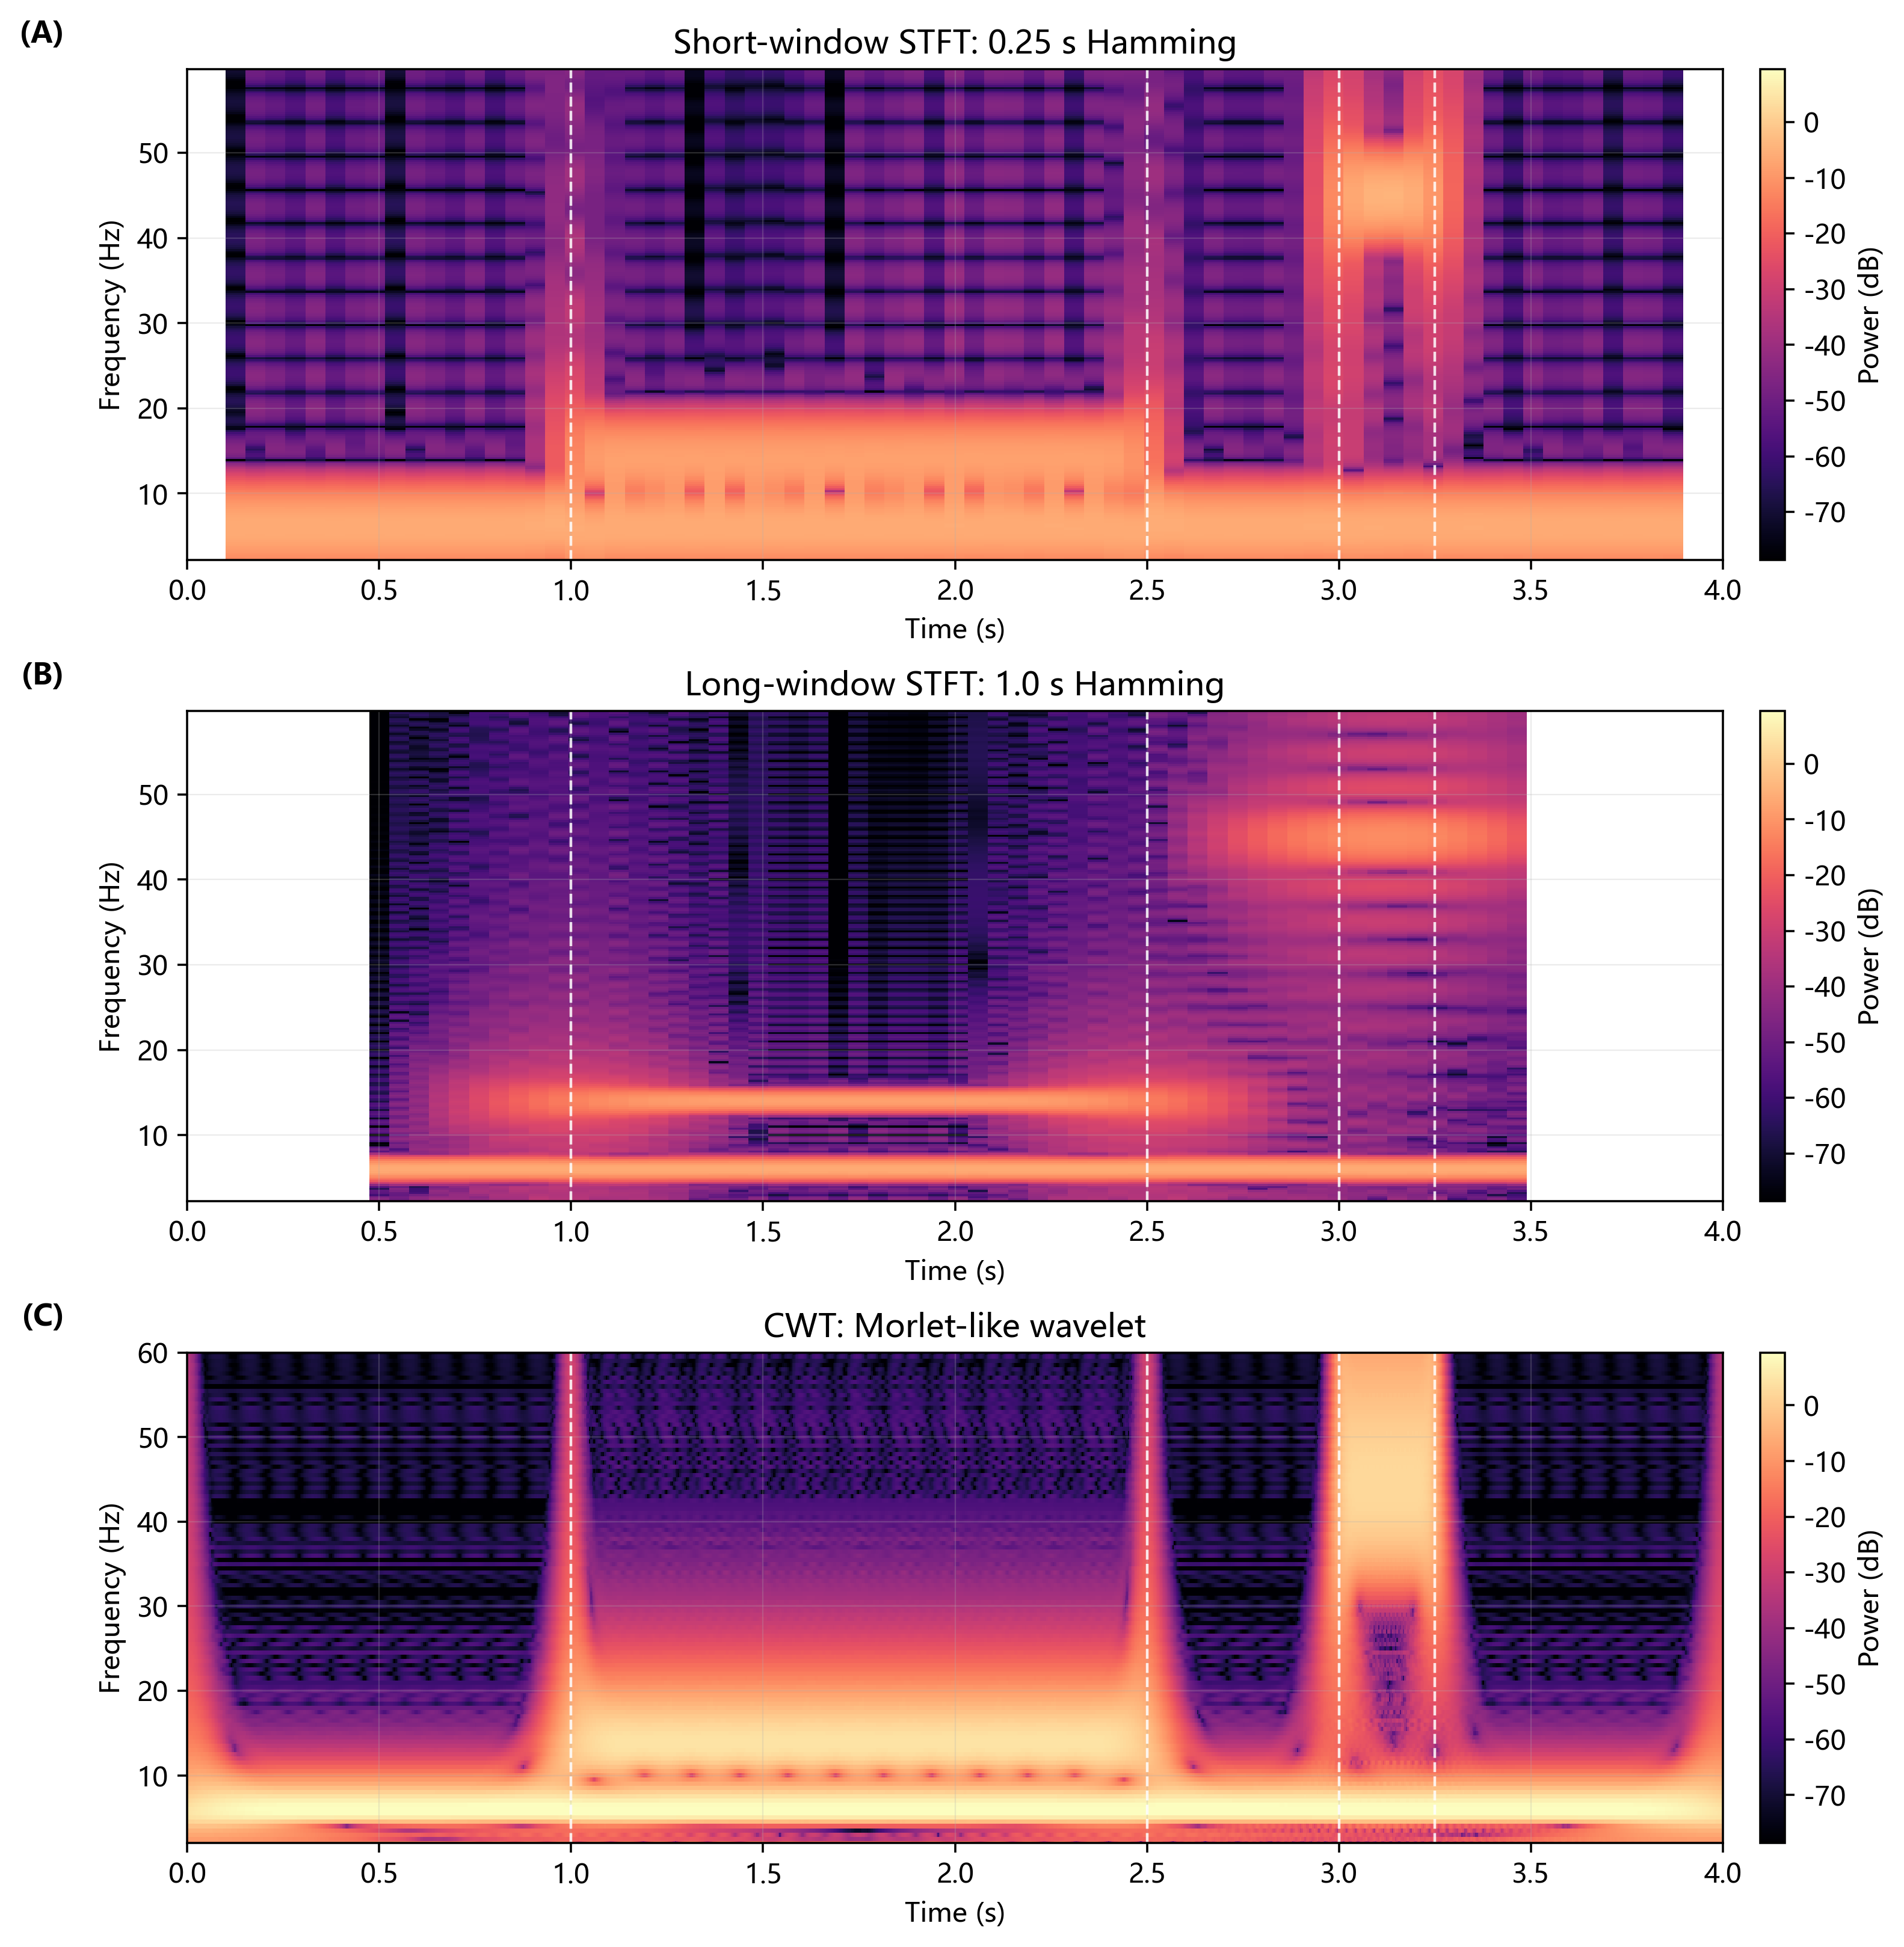
\includegraphics[width=0.96\textwidth]{exp3_x4_stft_cwt_compare.png}
\caption{Short-window STFT, long-window STFT, and CWT on the same $x_4$ signal. Fixed STFT windows emphasize different features, while CWT distributes resolution across scales.}
\label{fig:exp3-compare}
\end{figure}


Table \ref{tab:exp3-metrics} quantifies the same observation. Short-window STFT, long-window STFT, and CWT give 45 Hz spread widths of 0.156, 0.364, and 0.228 s; the CWT 6 Hz continuity ratio is 0.995.

\begin{table}[H]
\centering
\caption{Semi-quantitative comparison of STFT and CWT on the same signal.}
\label{tab:exp3-metrics}
\scriptsize
\resizebox{\textwidth}{!}{%
\begin{tabular}{lllll}
\toprule
Method & 45Hz peak(s) & Spread width(s) & 6Hz continuity & 6Hz CV\\
\midrule
STFT\_short & 3.142 & 0.156 & 1.000 & 0.018\\
STFT\_long & 3.100 & 0.364 & 1.000 & 0.003\\
CWT & 3.084 & 0.228 & 0.995 & 0.123\\
\bottomrule
\end{tabular}
}
\end{table}


Figure \ref{fig:exp3-mra-overview} verifies $x_\mathrm{MRA}$ before decomposition. The waveform shows superposed slow and fast oscillations; the spectrum confirms 1, 6, 12, and 45 Hz components; the CWT map shows that 45 Hz is a localized 2.4--2.8 s burst.

\begin{figure}[H]
\centering
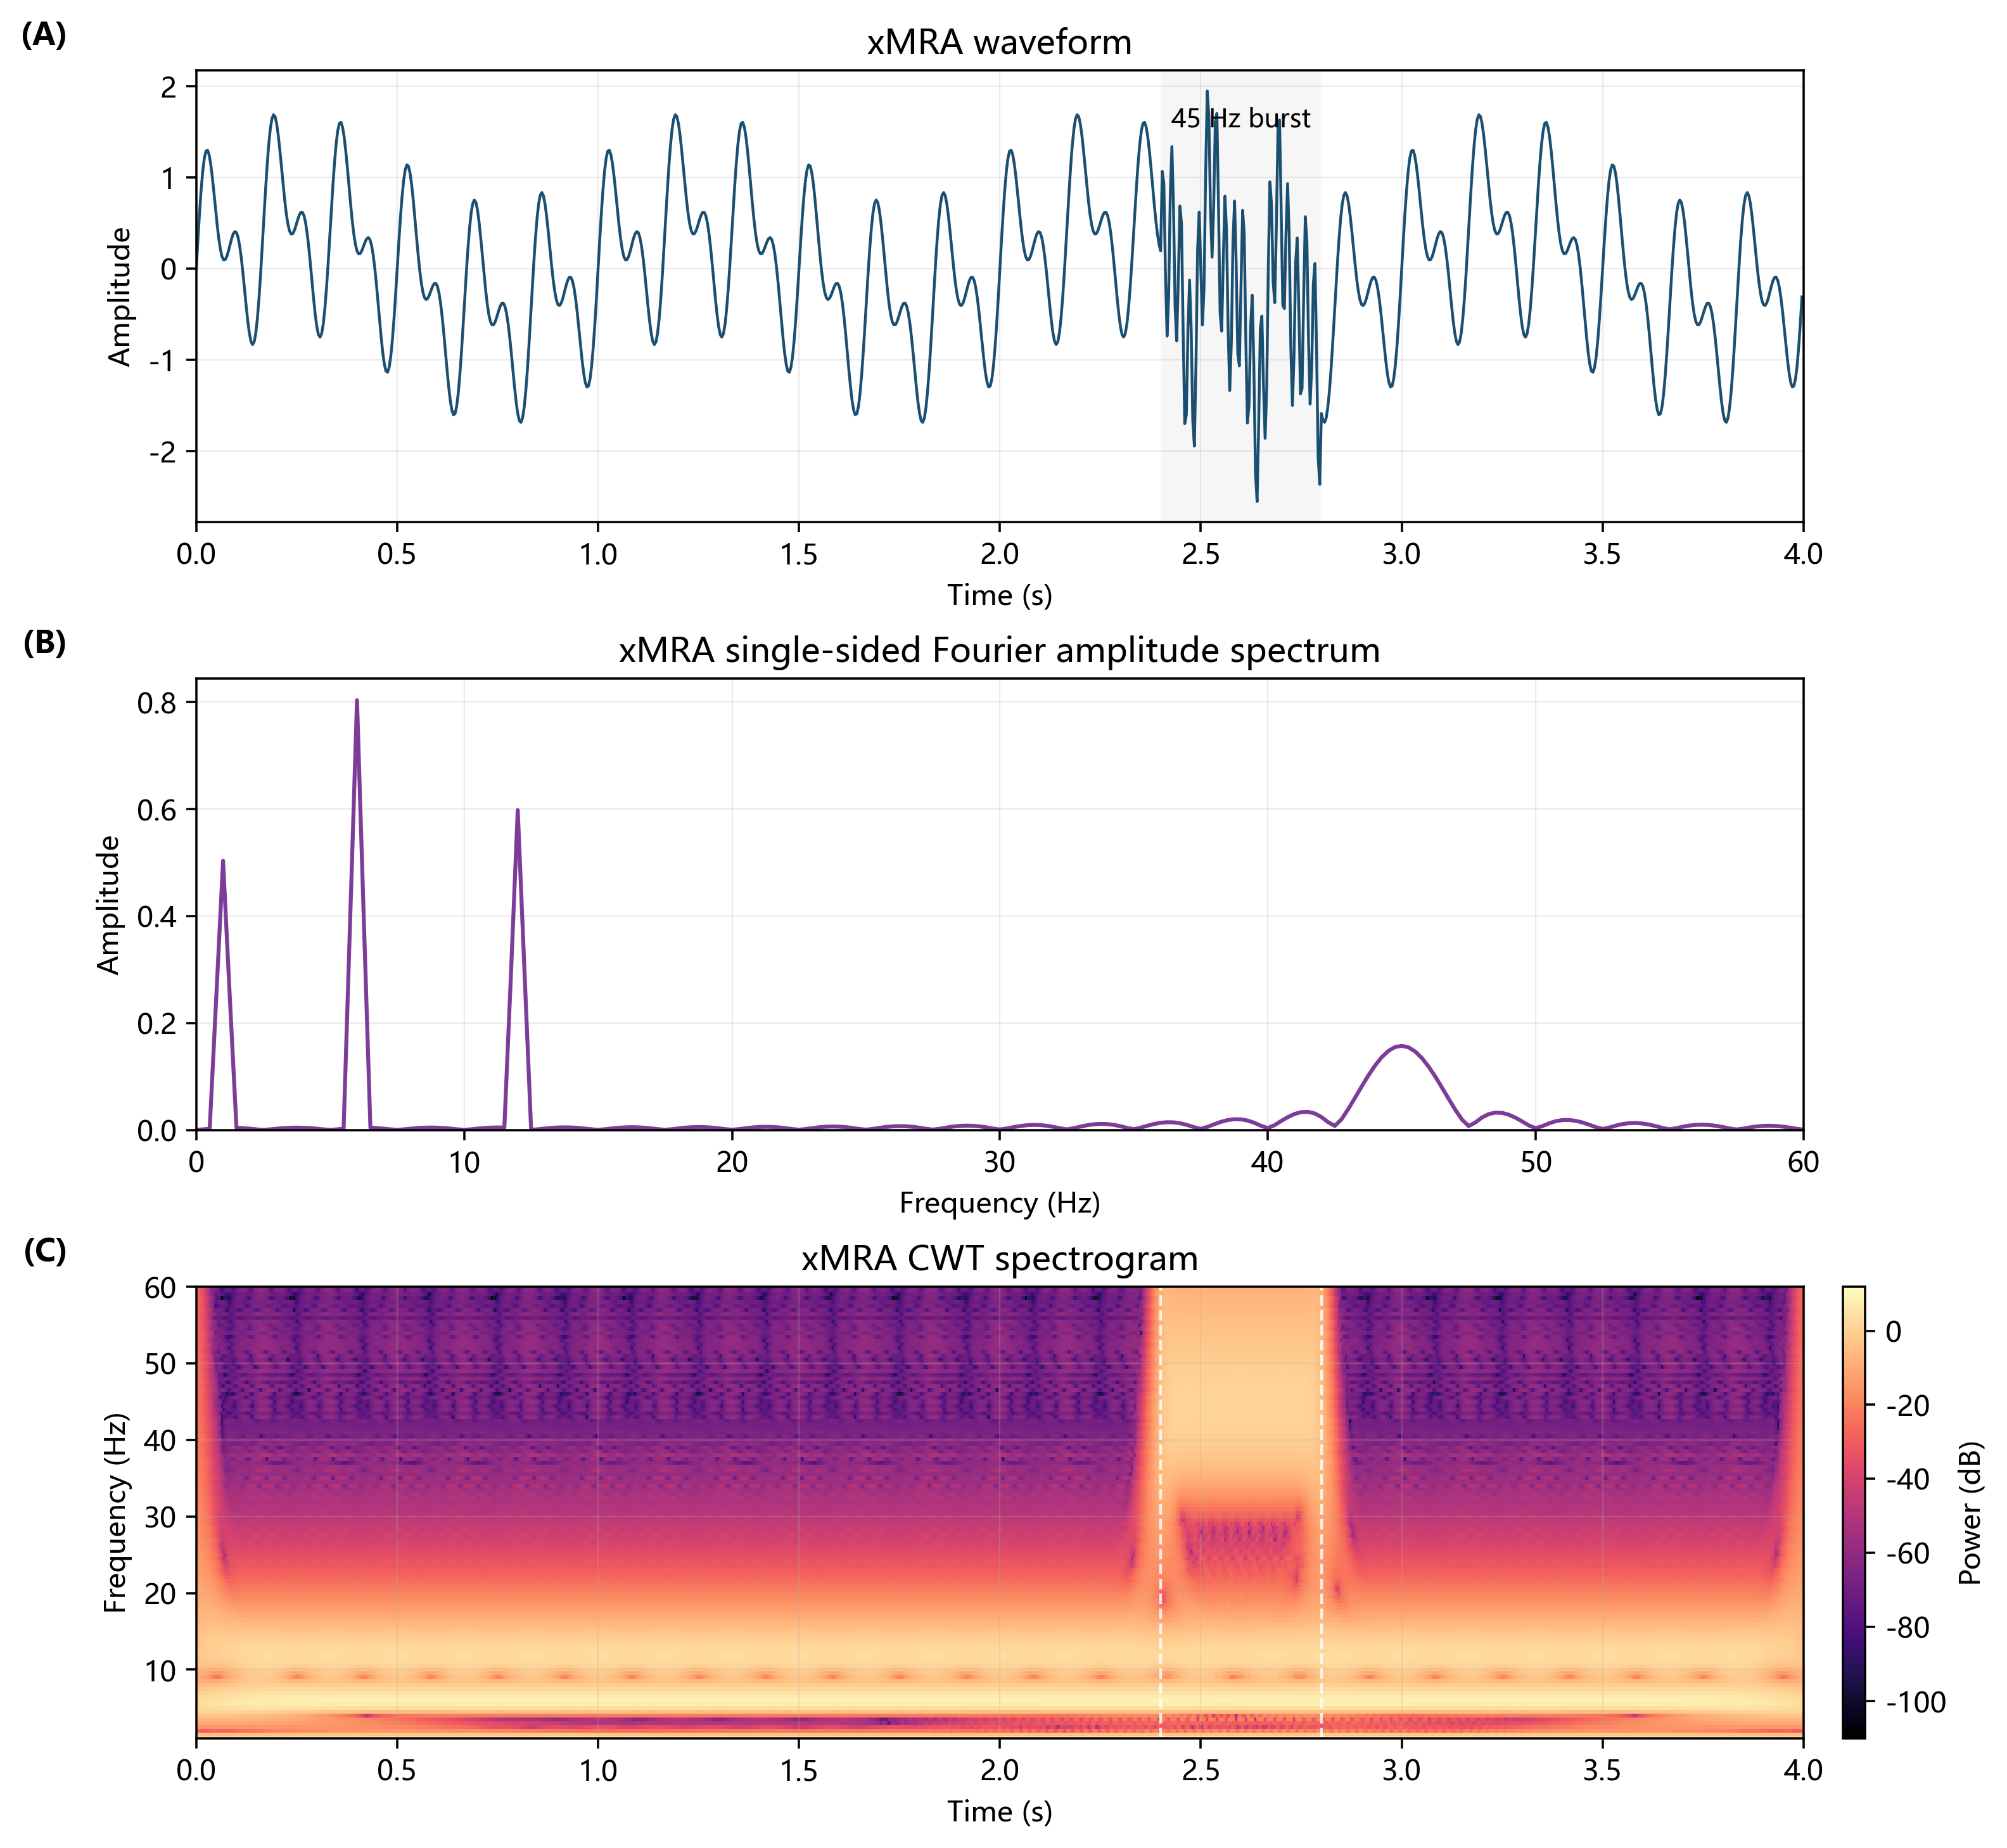
\includegraphics[width=0.96\textwidth]{exp3_mra_signal_fft_cwt.png}
\caption{$x_\mathrm{MRA}$ waveform, Fourier spectrum, and CWT map. The full spectrum shows 1, 6, 12, and 45 Hz components, while CWT localizes the 45 Hz burst.}
\label{fig:exp3-mra-overview}
\end{figure}


Figure \ref{fig:exp3-components} shows the six-level \texttt{sym6} decomposition. D2 aligns with the 45 Hz burst, D4 with the 12 Hz component, D5/D6 with the 6 Hz component and transition leakage, and A6 with the 1 Hz slow trend.

\begin{figure}[H]
\centering
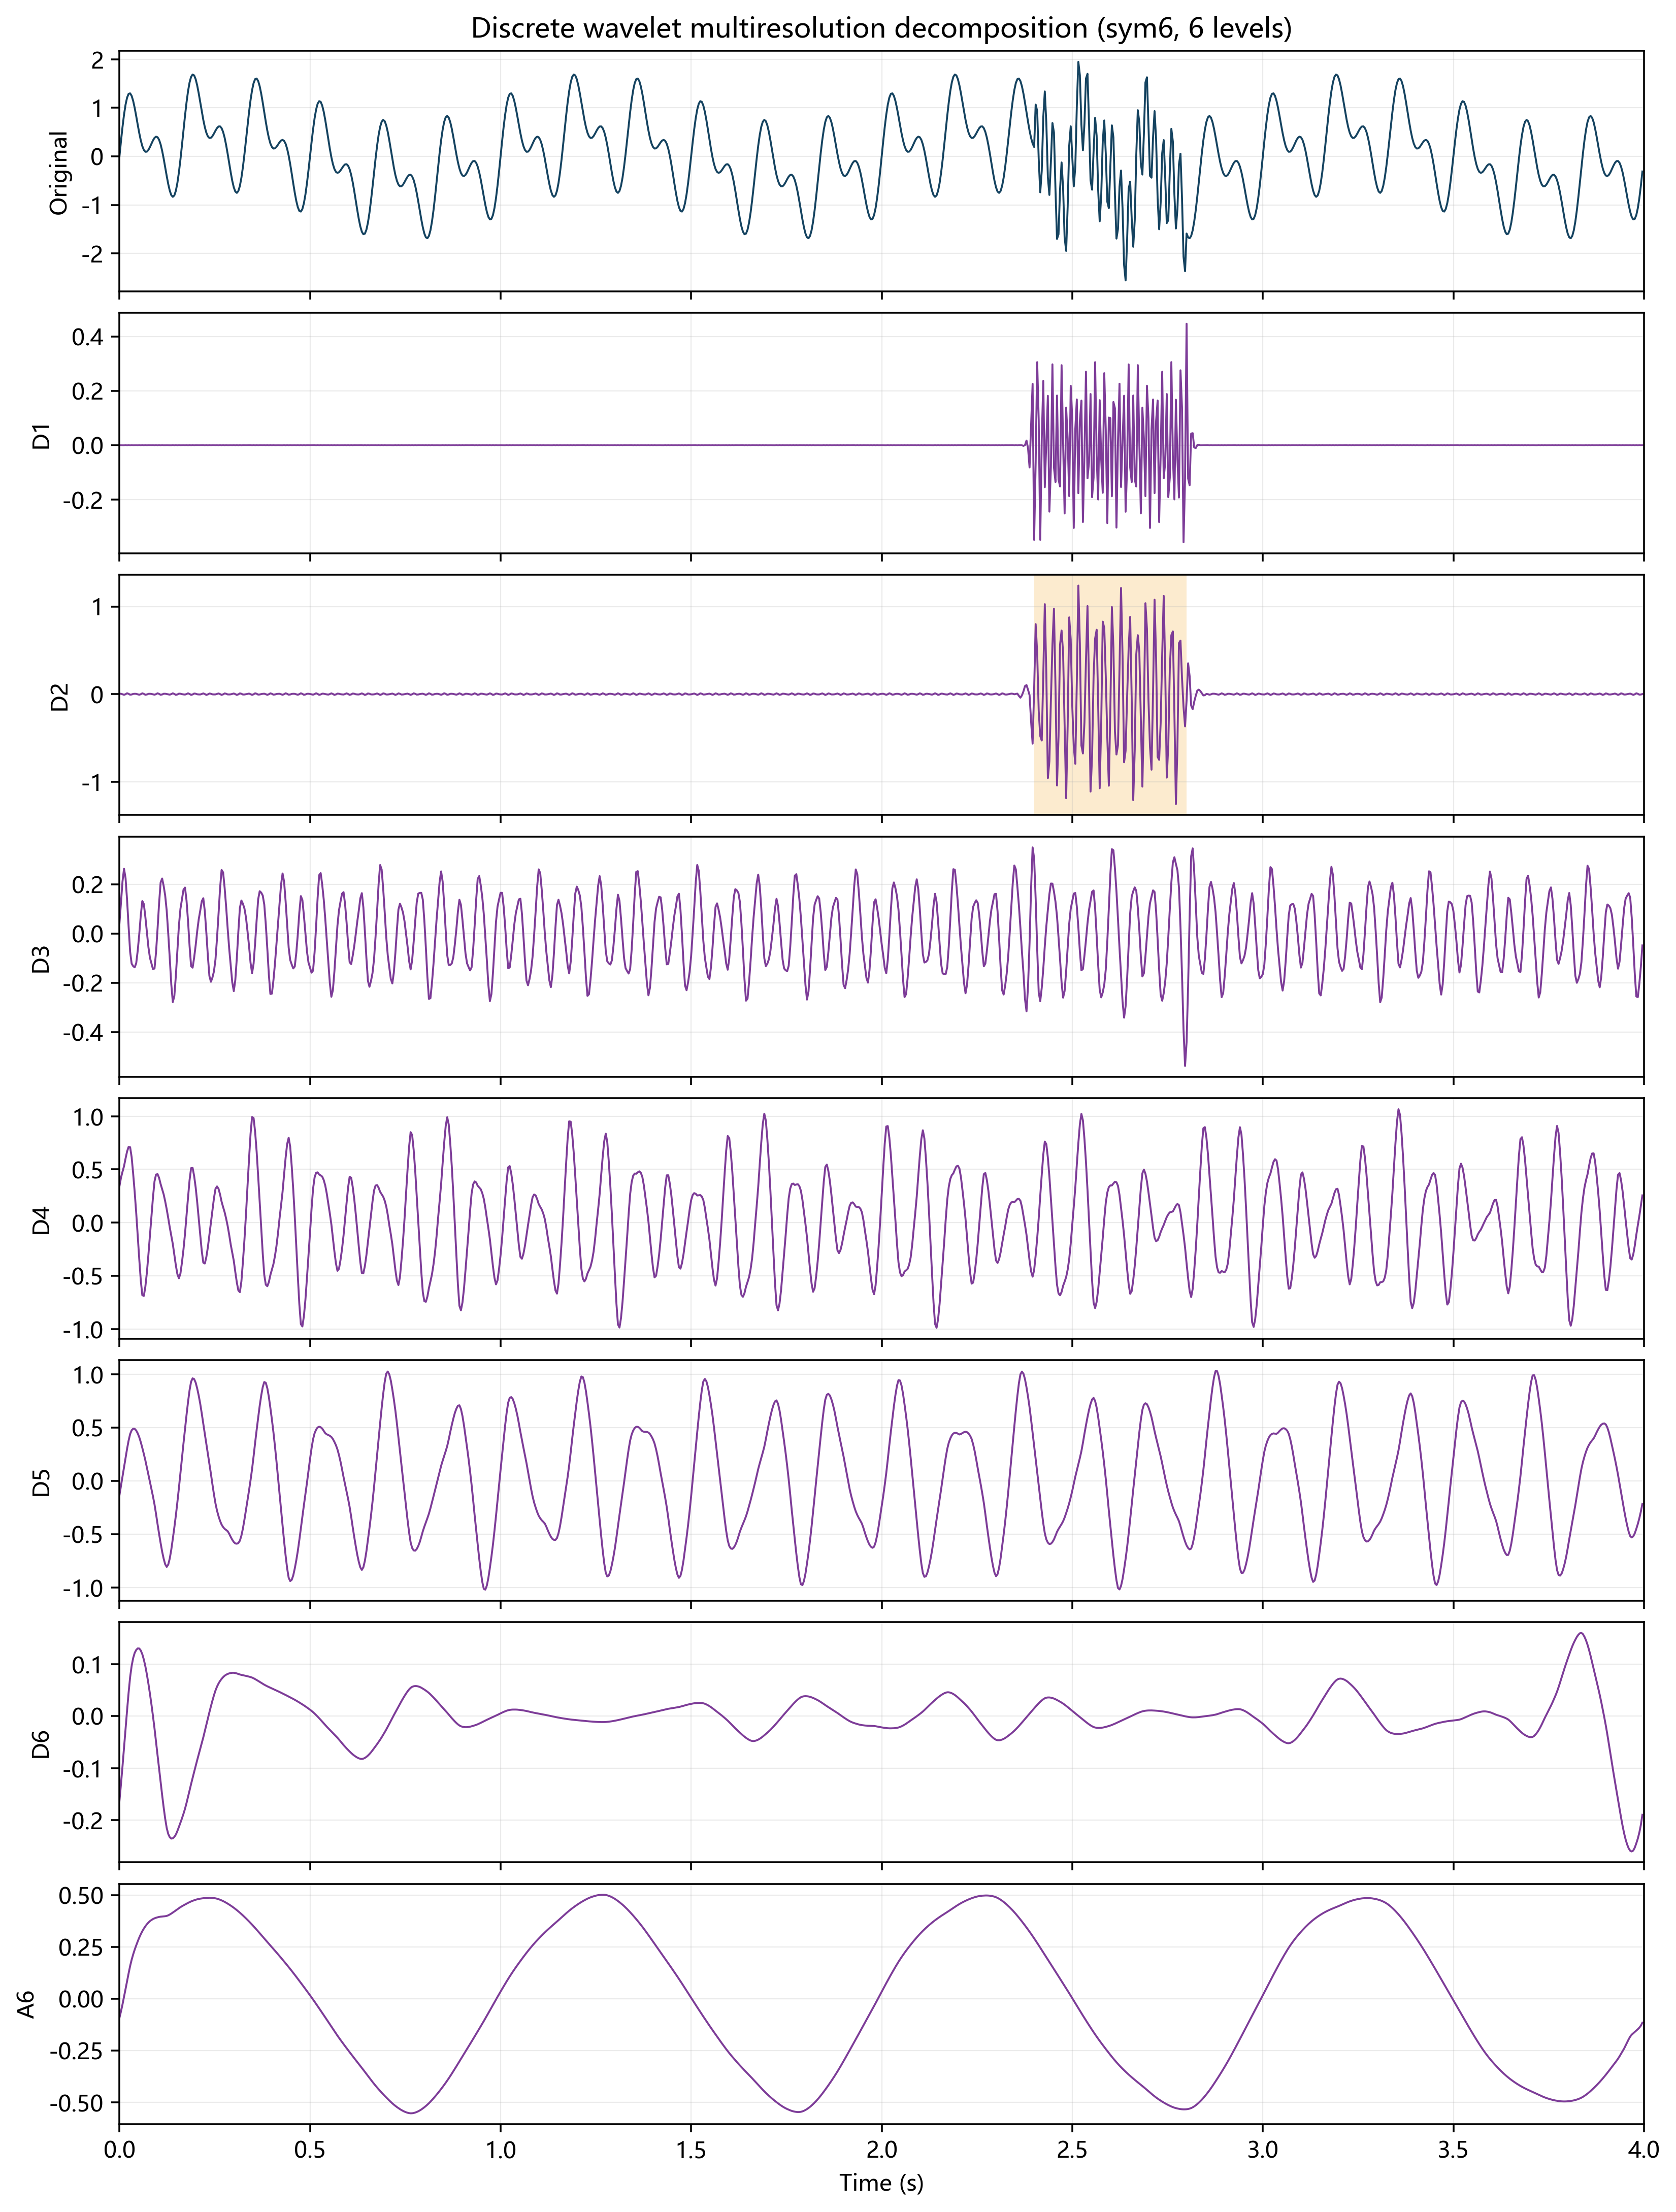
\includegraphics[width=0.96\textwidth]{exp3_mra_components.png}
\caption{Discrete wavelet multiresolution components of $x_\mathrm{MRA}$ using sym6 and six levels. D2 highlights the 45 Hz burst, while lower-frequency layers represent slower components.}
\label{fig:exp3-components}
\end{figure}


Table \ref{tab:exp3-bands} provides the approximate dyadic band mapping used for interpreting the components.

\begin{table}[H]
\centering
\caption{Approximate dyadic frequency bands for a six-level sym6 DWT.}
\label{tab:exp3-bands}
\scriptsize
\resizebox{\textwidth}{!}{%
\begin{tabular}{lll}
\toprule
Component & Low (Hz) & High (Hz)\\
\midrule
A6 & 0.00 & 1.95\\
D6 & 1.95 & 3.91\\
D5 & 3.91 & 7.81\\
D4 & 7.81 & 15.62\\
D3 & 15.62 & 31.25\\
D2 & 31.25 & 62.50\\
D1 & 62.50 & 125.00\\
\bottomrule
\end{tabular}
}
\end{table}


Figure \ref{fig:exp3-recon} illustrates reconstruction by selected layers. A6+D6+D5+D4 preserves the slow trend, 6 Hz, and about 12 Hz components, while D2 isolates the high-frequency burst. This shows that layer selection is also a frequency-content selection.

\begin{figure}[H]
\centering
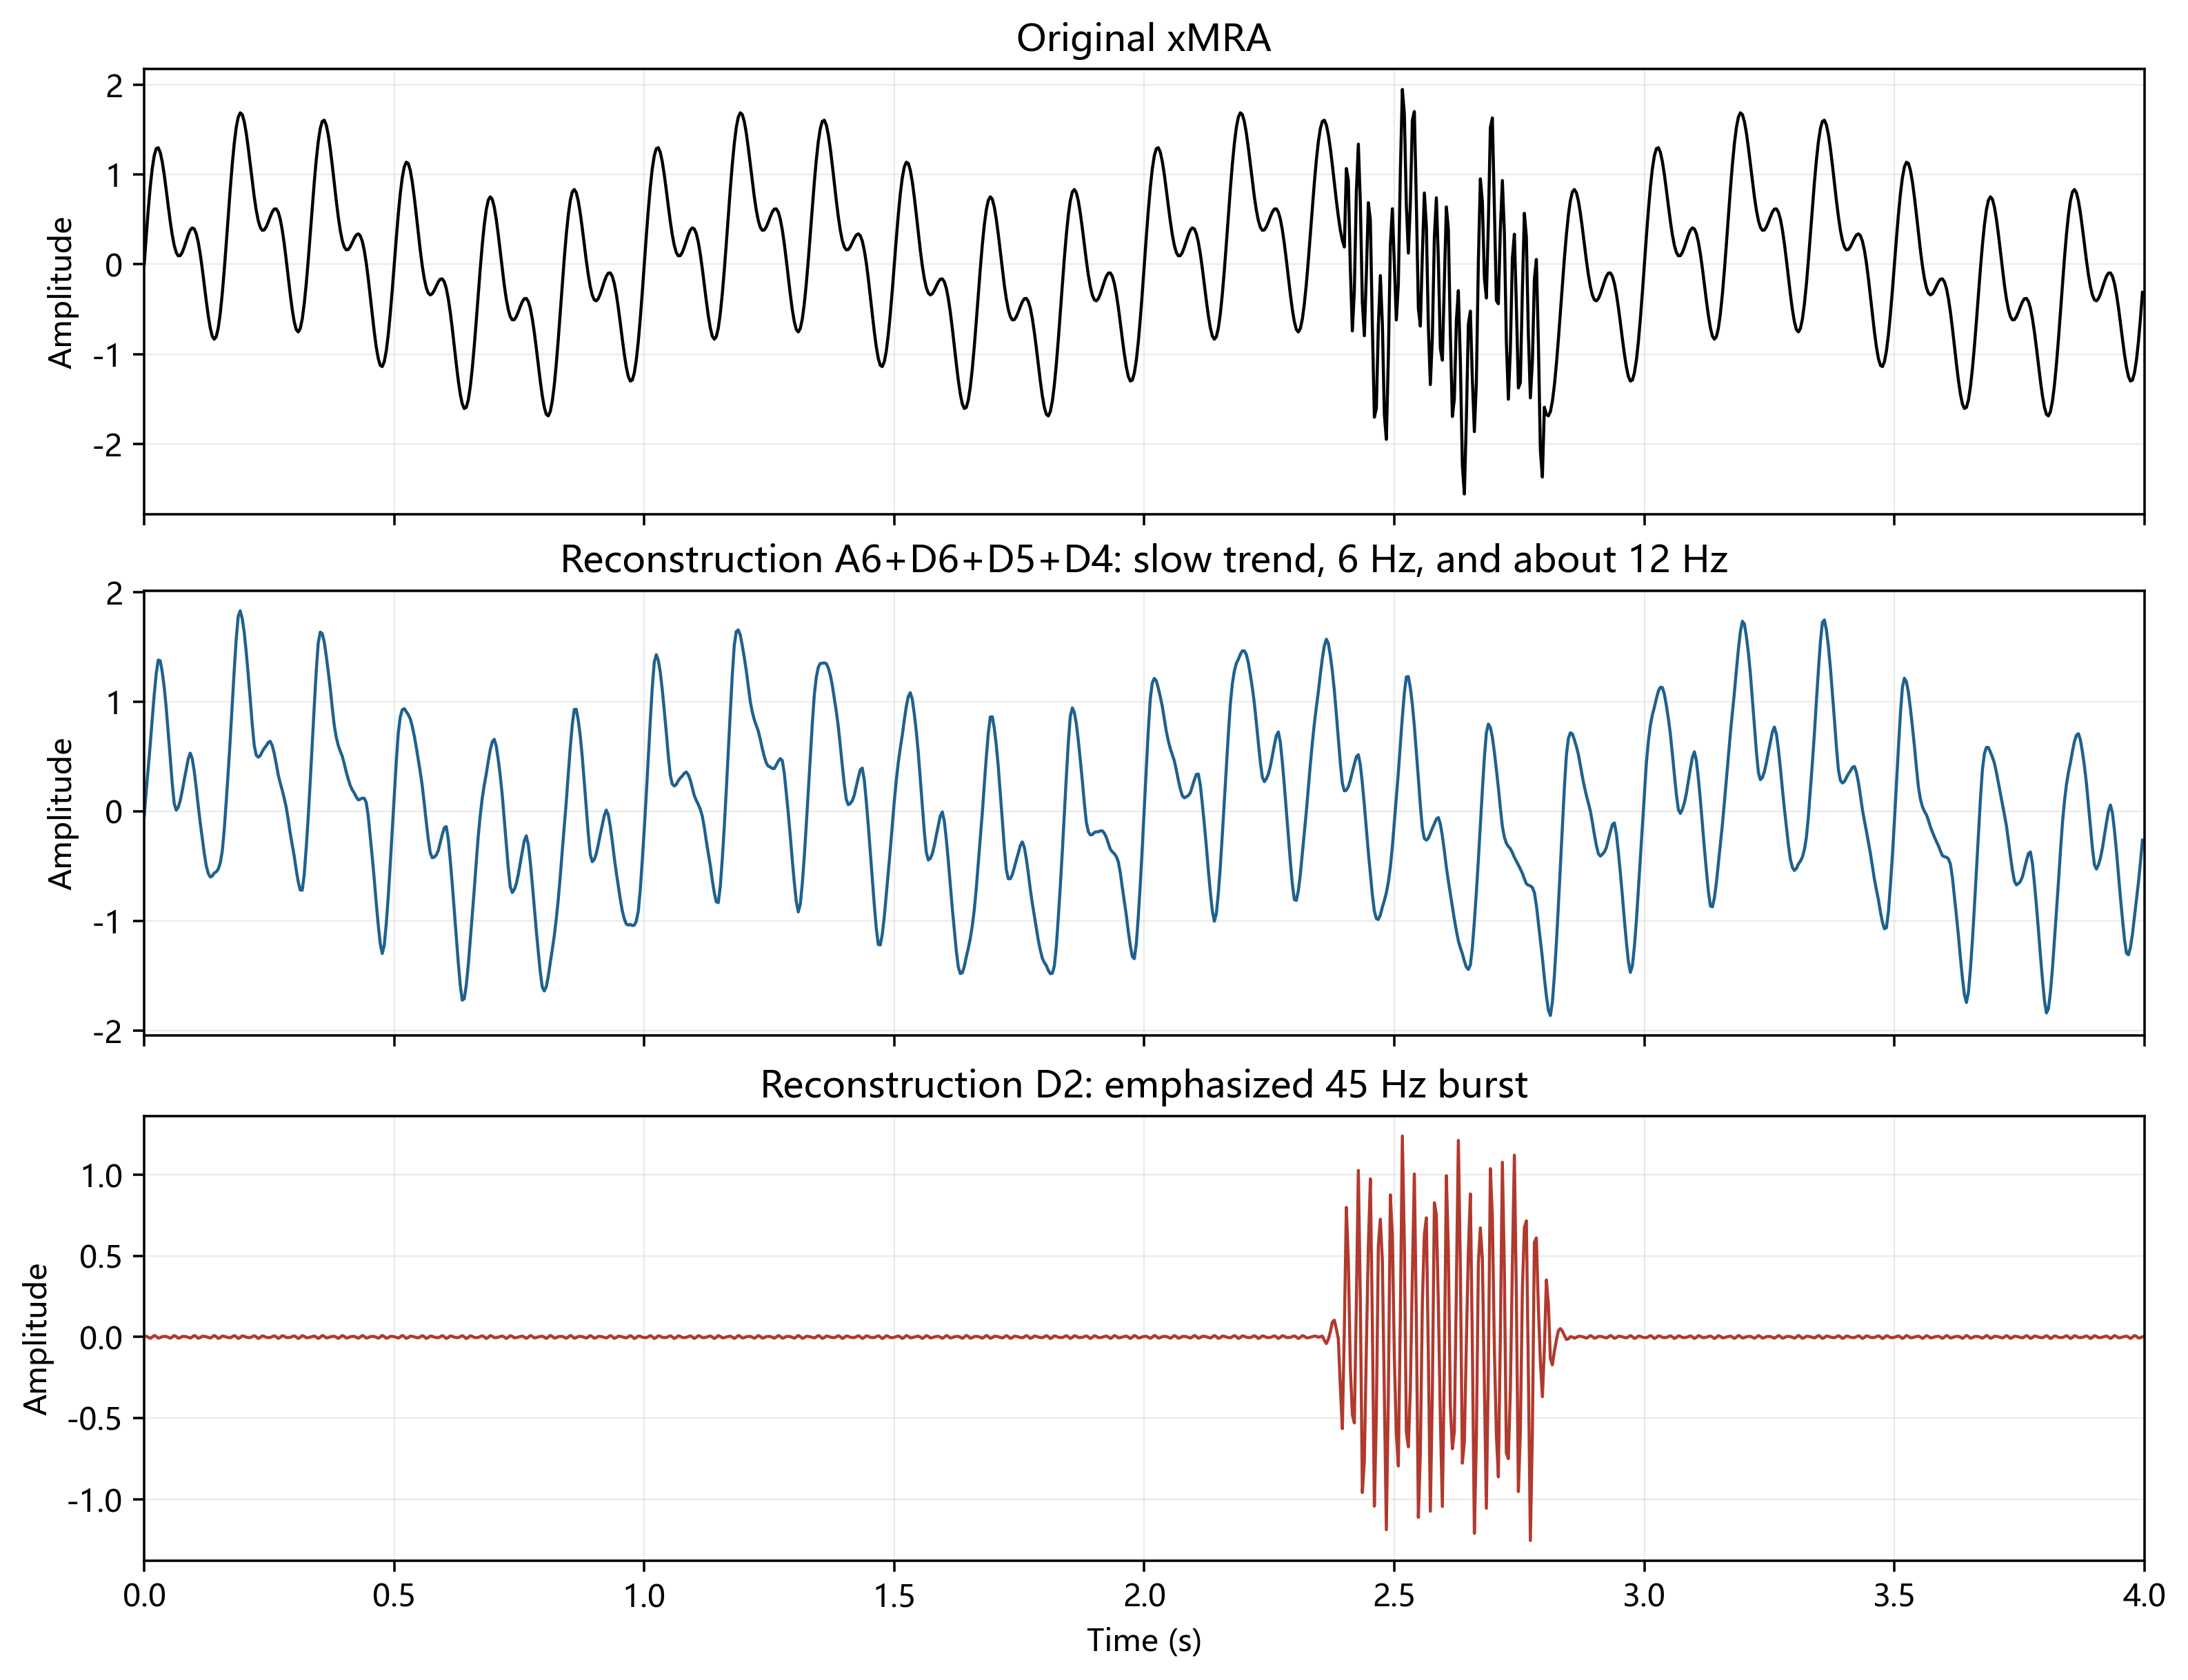
\includegraphics[width=0.96\textwidth]{exp3_mra_reconstruction.png}
\caption{Layer-based reconstructions of $x_\mathrm{MRA}$. A low/middle-band combination preserves slow and rhythmic components, while D2 emphasizes the high-frequency burst.}
\label{fig:exp3-recon}
\end{figure}


\subsection{Analysis and Discussion}
Figure \ref{fig:exp3-compare} demonstrates the limitation of fixed-window STFT. The short window is good for the high-frequency burst but less precise for the low-frequency band. The long window is good for low/middle-frequency stability but smears the burst. CWT is advantageous here because scale changes with frequency.

Figure \ref{fig:exp3-mra-overview} and Figure \ref{fig:exp3-components} show that DWT components should be interpreted by approximate frequency bands and time-local behavior. D2 captures the 45 Hz burst, D4 captures much of the 12 Hz component, D5 and D6 participate in the 6 Hz rhythm, and A6 captures the slow 1 Hz trend. The components are not perfectly isolated because practical wavelet filters have transition bands.

\paragraph{Question: STFT and CWT both generate time-frequency maps. How do their analysis principles differ?}
Answer: STFT uses a fixed-length window for all frequencies. CWT changes scale with frequency: high frequencies are observed with shorter wavelets and low frequencies with longer wavelets. Thus the two methods allocate time-frequency resolution differently.

\paragraph{Question: Why do short-window and long-window STFT emphasize different features of the same signal?}
Answer: A short window has better temporal localization and poorer frequency resolution; a long window has better frequency resolution and poorer temporal localization. Therefore the same signal can look different under the two settings.

\paragraph{Question: What is the main advantage of CWT in this experiment, and what should still be interpreted cautiously?}
Answer: CWT simultaneously shows a continuous low-frequency component and a localized high-frequency burst better than a single fixed STFT window. However, wavelet choice, scale sampling, edge effects, and normalization all affect the map, so CWT is still a parameterized estimate rather than absolute truth.

\paragraph{Question: Why does multiscale CWT not mean CWT is always superior to STFT?}
Answer: Some tasks require a fixed analysis block, simple latency control, or comparability with conventional spectral estimates. CWT introduces additional choices and can produce boundary artifacts or over-smoothed structures if used carelessly.

\paragraph{Question: What is the risk of drawing conclusions from one parameter setting only?}
Answer: One setting may emphasize some components and suppress others. A short STFT may understate low-frequency stability, a long STFT may overstate burst duration, and a CWT map may be affected by scale and edge choices. Robust conclusions should combine multiple parameter checks and quantitative metrics.

\FloatBarrier
\clearpage
\section{Experiment 4: ERD Time-Frequency Features in Real Motor Imagery EEG}
\subsection{Data and Preprocessing Methods}
In the Lee2019/OpenBMI motor imagery paradigm, each trial begins with a fixation cross, then a left or right arrow cue instructs the participant to imagine the corresponding hand grasp. EEG was sampled at 1000 Hz with 62 scalp channels. The analysis locates C3, C4, Cz, FC3, FC4, CP3, and CP4 by channel name rather than assuming fixed column numbers. Figure \ref{fig:exp4-pipeline} summarizes the workflow: select channels, apply a 1--45 Hz zero-phase Butterworth filter, epoch trials from $[-1,4]$ s relative to cue, and downsample to 250 Hz.

For each trial, CWT power is baseline-corrected as
\begin{equation}
D(t,f)=10\log_{10}\frac{P(t,f)}{P_\mathrm{baseline}(f)} ,
\end{equation}
where $P_\mathrm{baseline}(f)$ is the mean power over $[-0.8,-0.2]$ s at the same frequency. Negative dB values indicate power decreases relative to the pre-cue baseline and are the primary ERD evidence. The task metric window is $[0.5,3.5]$ s. The workflow computes CWT power and baseline correction per trial before condition averaging to avoid cancellation of non-phase-locked rhythms.

The lateralization metric is
\begin{equation}
L_b=\overline{D}_{C3,b}-\overline{D}_{C4,b} .
\end{equation}
For left-hand imagery, stronger C4 ERD means C4 is more negative, so $L_b$ tends to be positive. For right-hand imagery, stronger C3 ERD makes $L_b$ negative.

Figure \ref{fig:exp4-epoch} defines the epoch, baseline, and task metric windows. The baseline precedes cue onset, and the task window starts at 0.5 s to reduce cue-locked visual and preparation effects.

\begin{figure}[H]
\centering
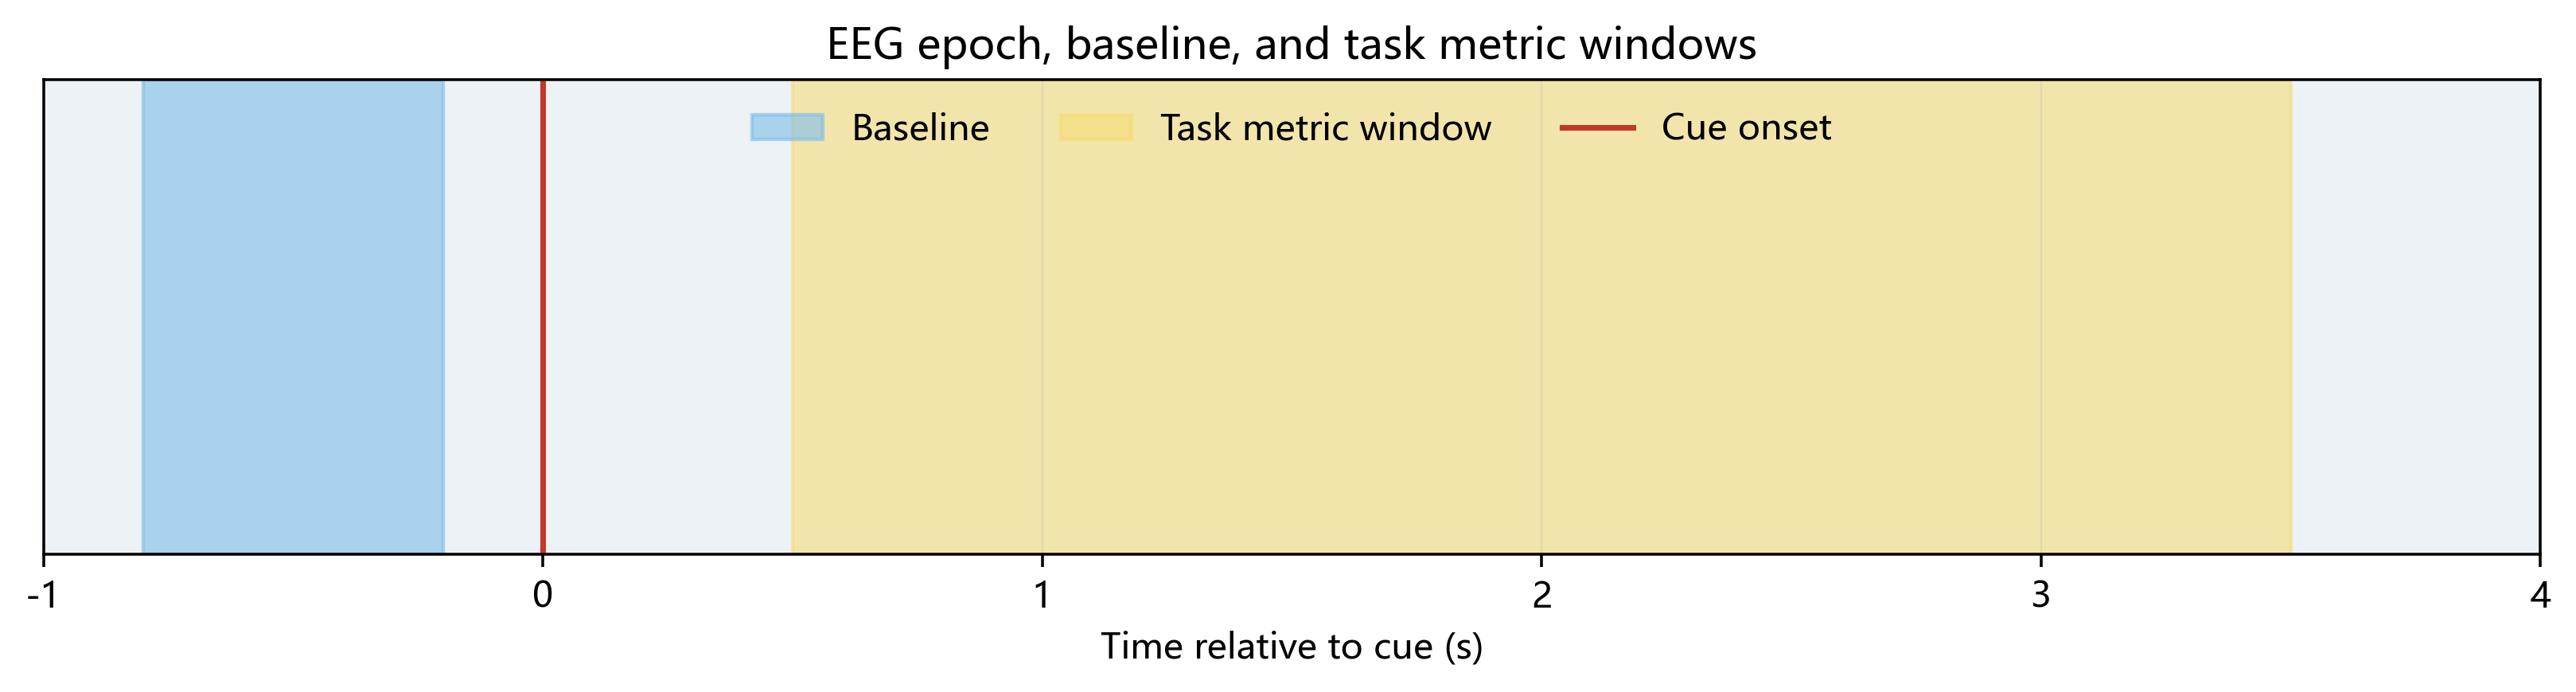
\includegraphics[width=0.82\textwidth]{exp4_epoch_design.png}
\caption{EEG epoch design with baseline and task metric windows.}
\label{fig:exp4-epoch}
\end{figure}


Figure \ref{fig:exp4-pipeline} emphasizes that the time-frequency power is computed per trial and then averaged by condition.

\begin{figure}[H]
\centering
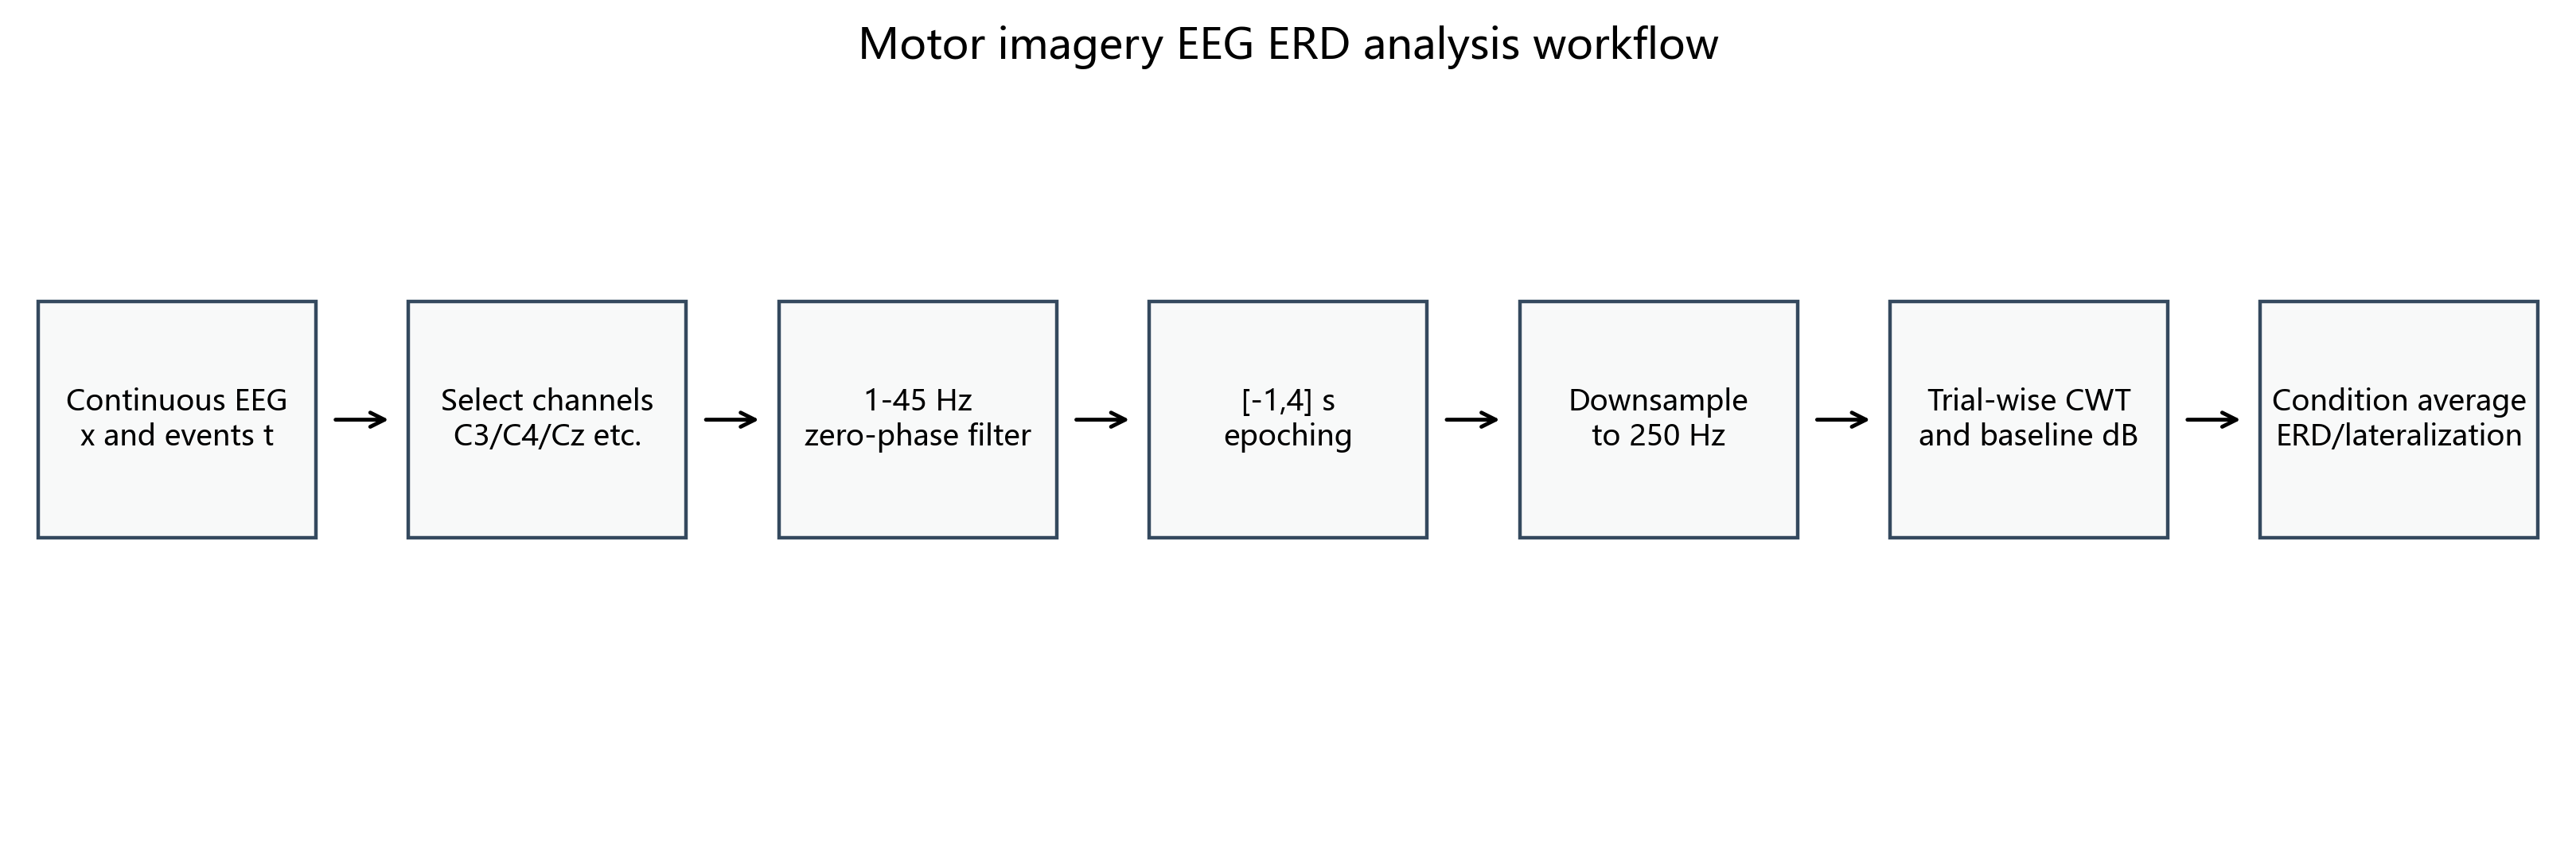
\includegraphics[width=0.92\textwidth]{exp4_processing_pipeline.png}
\caption{Motor imagery EEG ERD analysis workflow.}
\label{fig:exp4-pipeline}
\end{figure}


Table \ref{tab:exp4-meta} verifies the data structure and selected channel indices. Table \ref{tab:exp4-counts} confirms that the main combined analysis contains 100 left-hand and 100 right-hand trials for C3/C4.

\begin{table}[H]
\centering
\caption{EEG data structure and preprocessing metadata.}
\label{tab:exp4-meta}
\scriptsize
\resizebox{\textwidth}{!}{%
\begin{tabular}{lllllll}
\toprule
Split & Original fs & Target fs & Events & Kept epochs & Channel indices & NaNs\\
\midrule
EEG\_MI\_train & 1000.000 & 250.000 & 100.000 & 100.000 & [13, 15, 14, 33, 34, 39, 41] & 0.000\\
EEG\_MI\_test & 1000.000 & 250.000 & 100.000 & 100.000 & [13, 15, 14, 33, 34, 39, 41] & 0.000\\
\bottomrule
\end{tabular}
}
\end{table}


\begin{table}[H]
\centering
\caption{Number of C3/C4 trials entering condition averages.}
\label{tab:exp4-counts}
\scriptsize
\resizebox{\textwidth}{!}{%
\begin{tabular}{llll}
\toprule
Split & Condition & Channel & Trials\\
\midrule
all & left & C3 & 100\\
all & left & C4 & 100\\
all & right & C3 & 100\\
all & right & C4 & 100\\
train & left & C3 & 50\\
train & left & C4 & 50\\
train & right & C3 & 50\\
train & right & C4 & 50\\
test & left & C3 & 50\\
test & left & C4 & 50\\
test & right & C3 & 50\\
test & right & C4 & 50\\
\bottomrule
\end{tabular}
}
\end{table}


Figure \ref{fig:exp4-qc} reports descriptive quality control. Peak-to-peak amplitude is used as a descriptive reference rather than a result-driven rejection rule.

\begin{figure}[H]
\centering
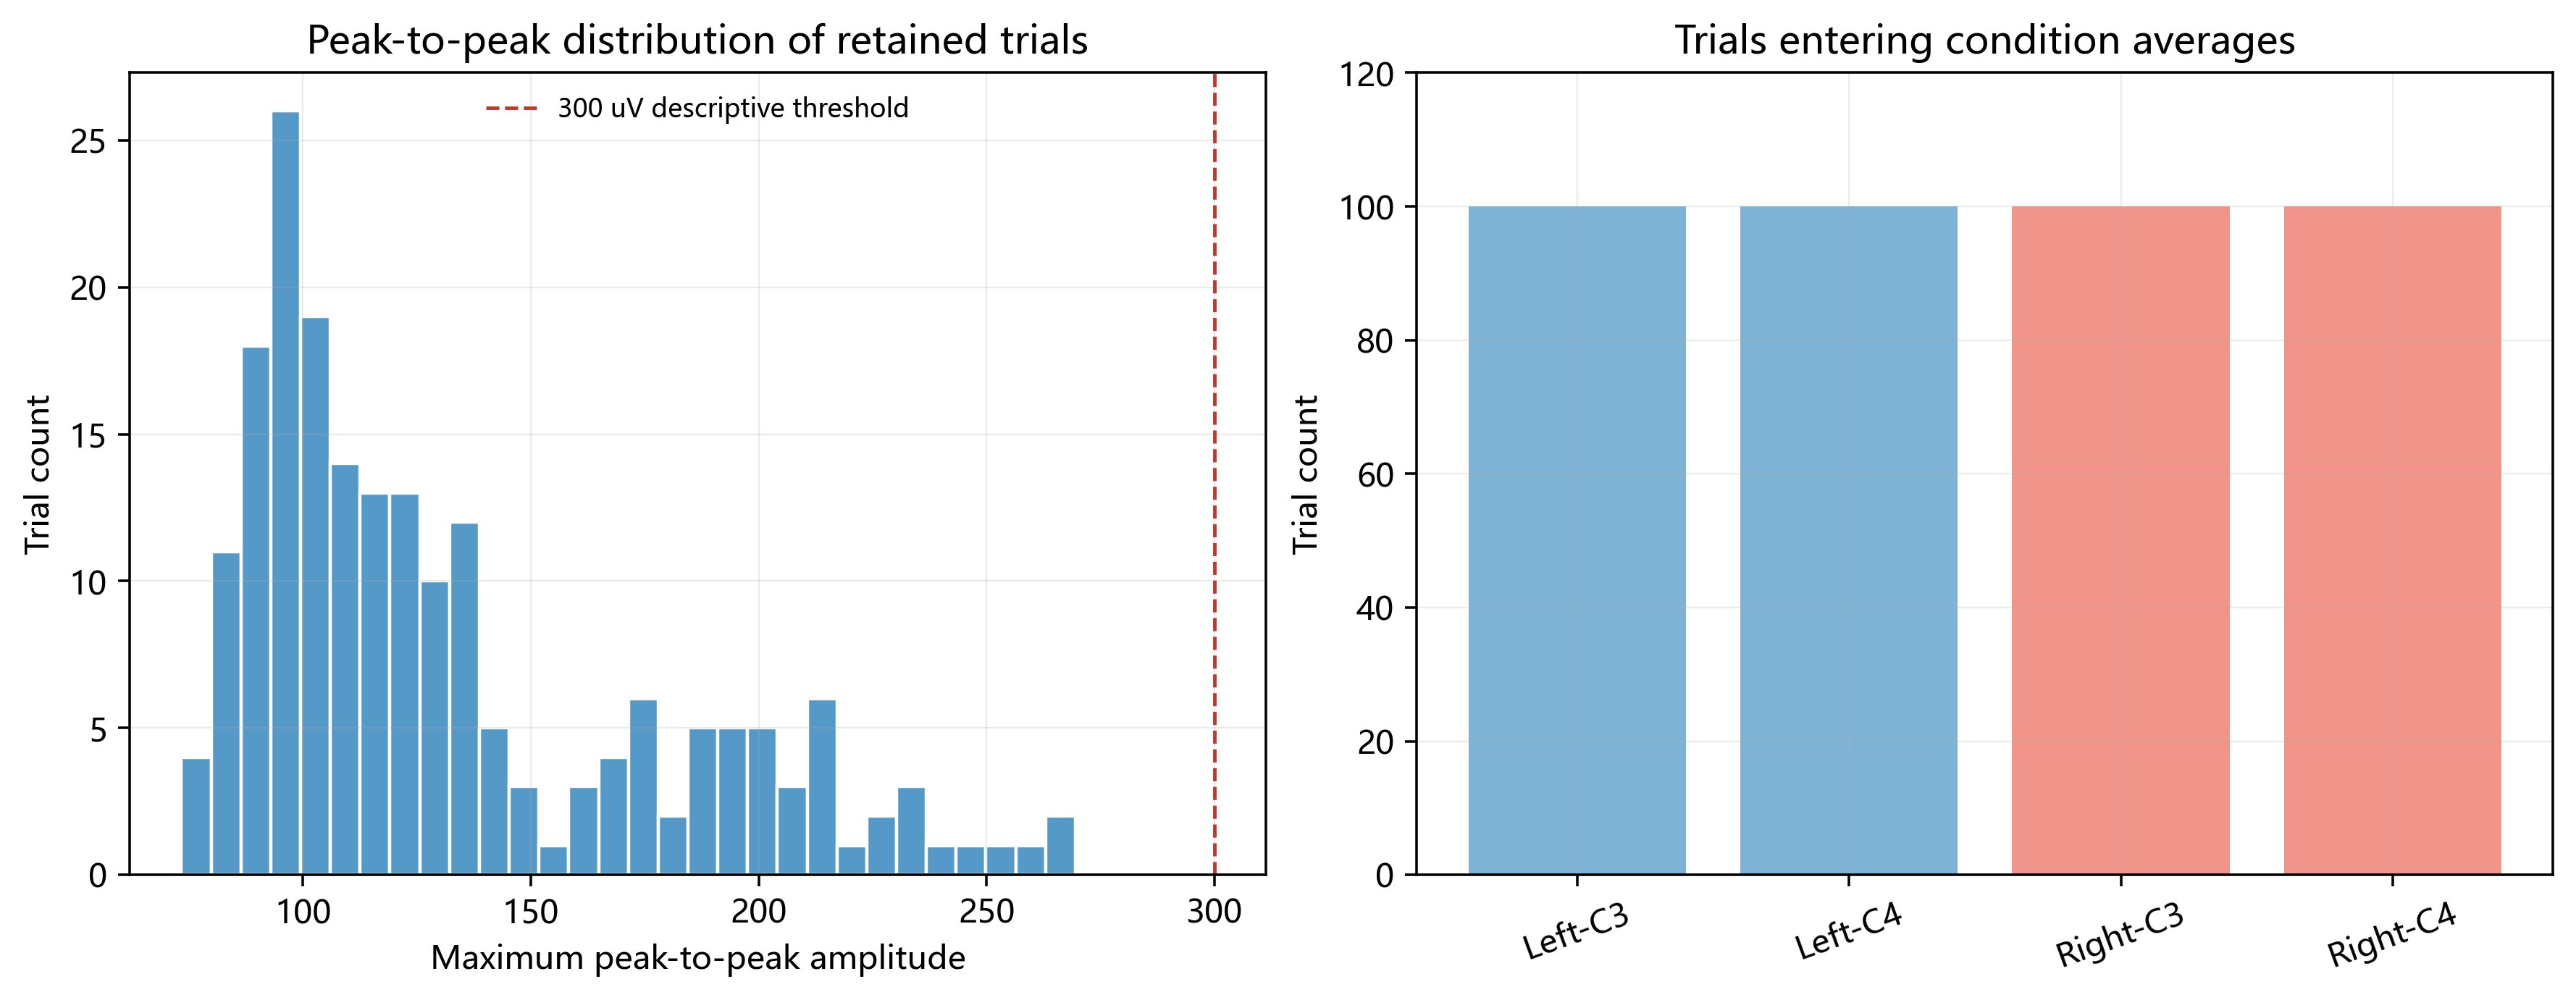
\includegraphics[width=0.90\textwidth]{exp4_quality_control.png}
\caption{EEG quality-control summary: peak-to-peak distribution and trial counts entering condition averages.}
\label{fig:exp4-qc}
\end{figure}


\Needspace{0.72\textheight}
\subsection{Time-Frequency and Lateralization Results}
Figure \ref{fig:exp4-tfr} is the core ERD map. Negative values indicate power below pre-cue baseline. Blue regions in the mu and beta ranges provide ERD evidence. Comparing C3 and C4 within each condition is the first step in judging lateralization.

\begin{figure}[H]
\centering
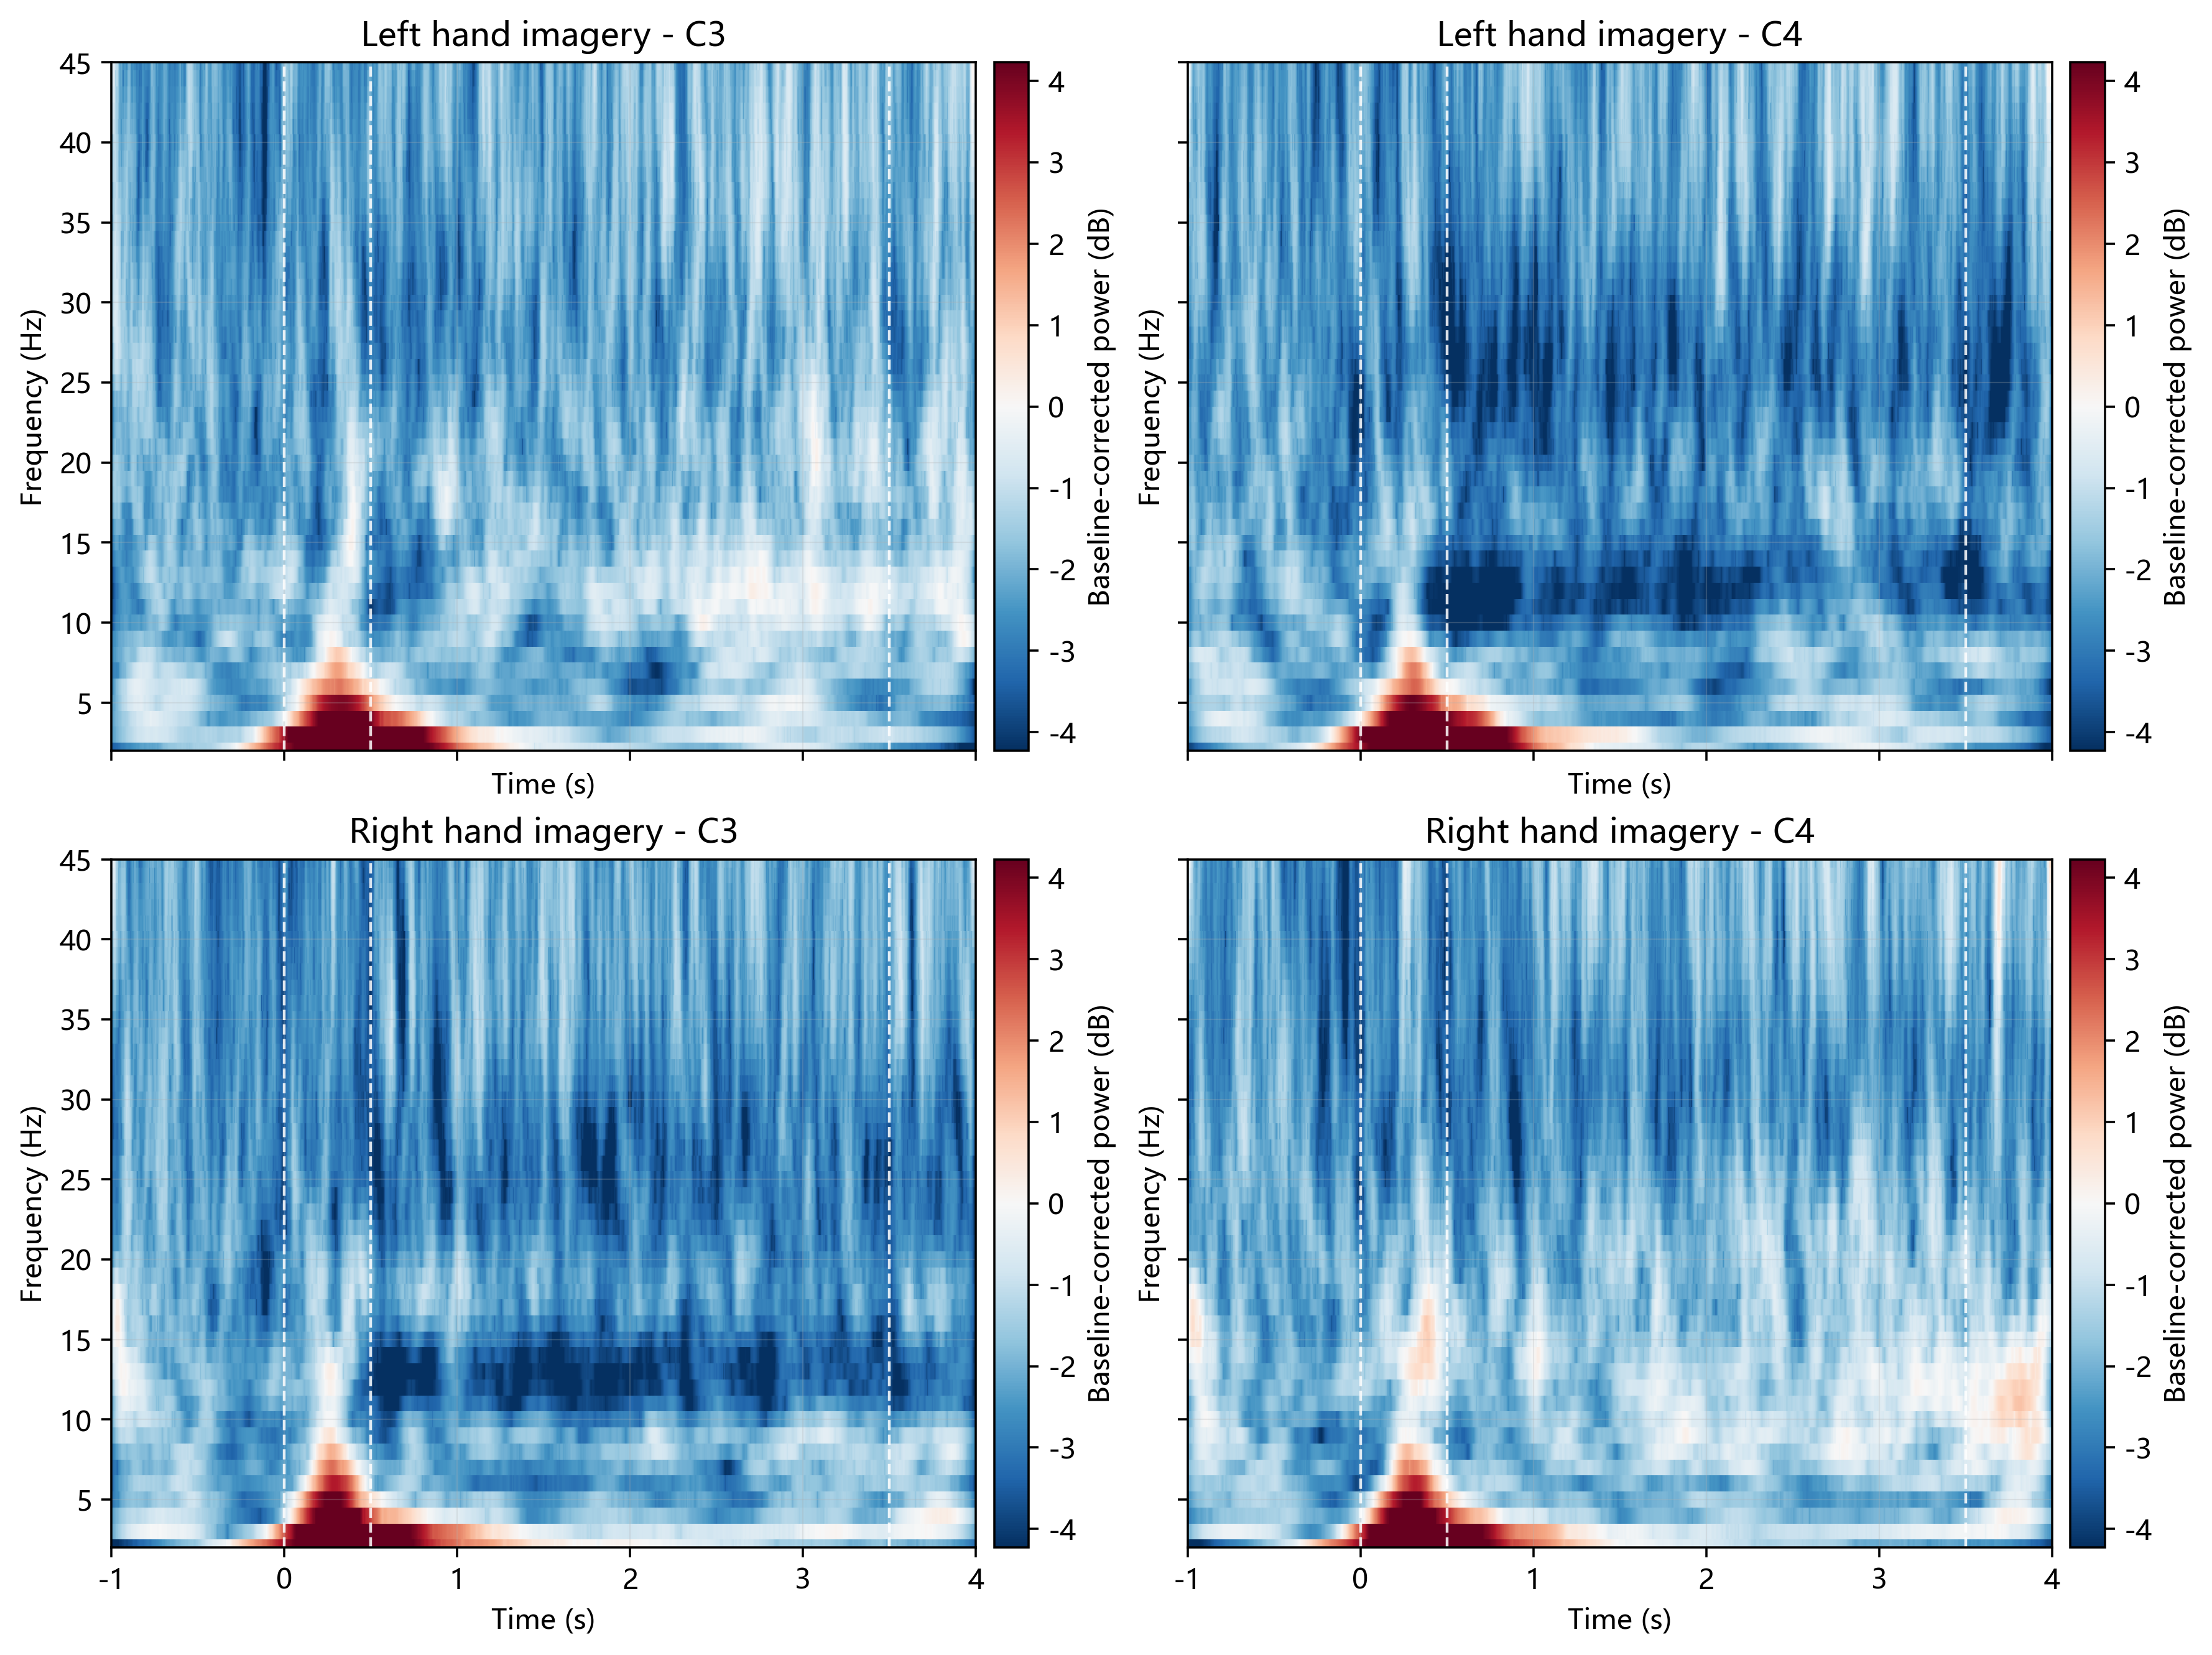
\includegraphics[width=0.96\textwidth]{exp4_c3_c4_erd_tfr.png}
\caption{Baseline-corrected CWT maps for C3/C4 under left- and right-hand motor imagery. Negative values indicate ERD.}
\label{fig:exp4-tfr}
\end{figure}


Figure \ref{fig:exp4-diff} displays C3-C4 directly. The sign must be interpreted together with ERD negativity: positive C3-C4 in left imagery can indicate stronger C4 ERD, and negative C3-C4 in right imagery can indicate stronger C3 ERD.

\begin{figure}[H]
\centering
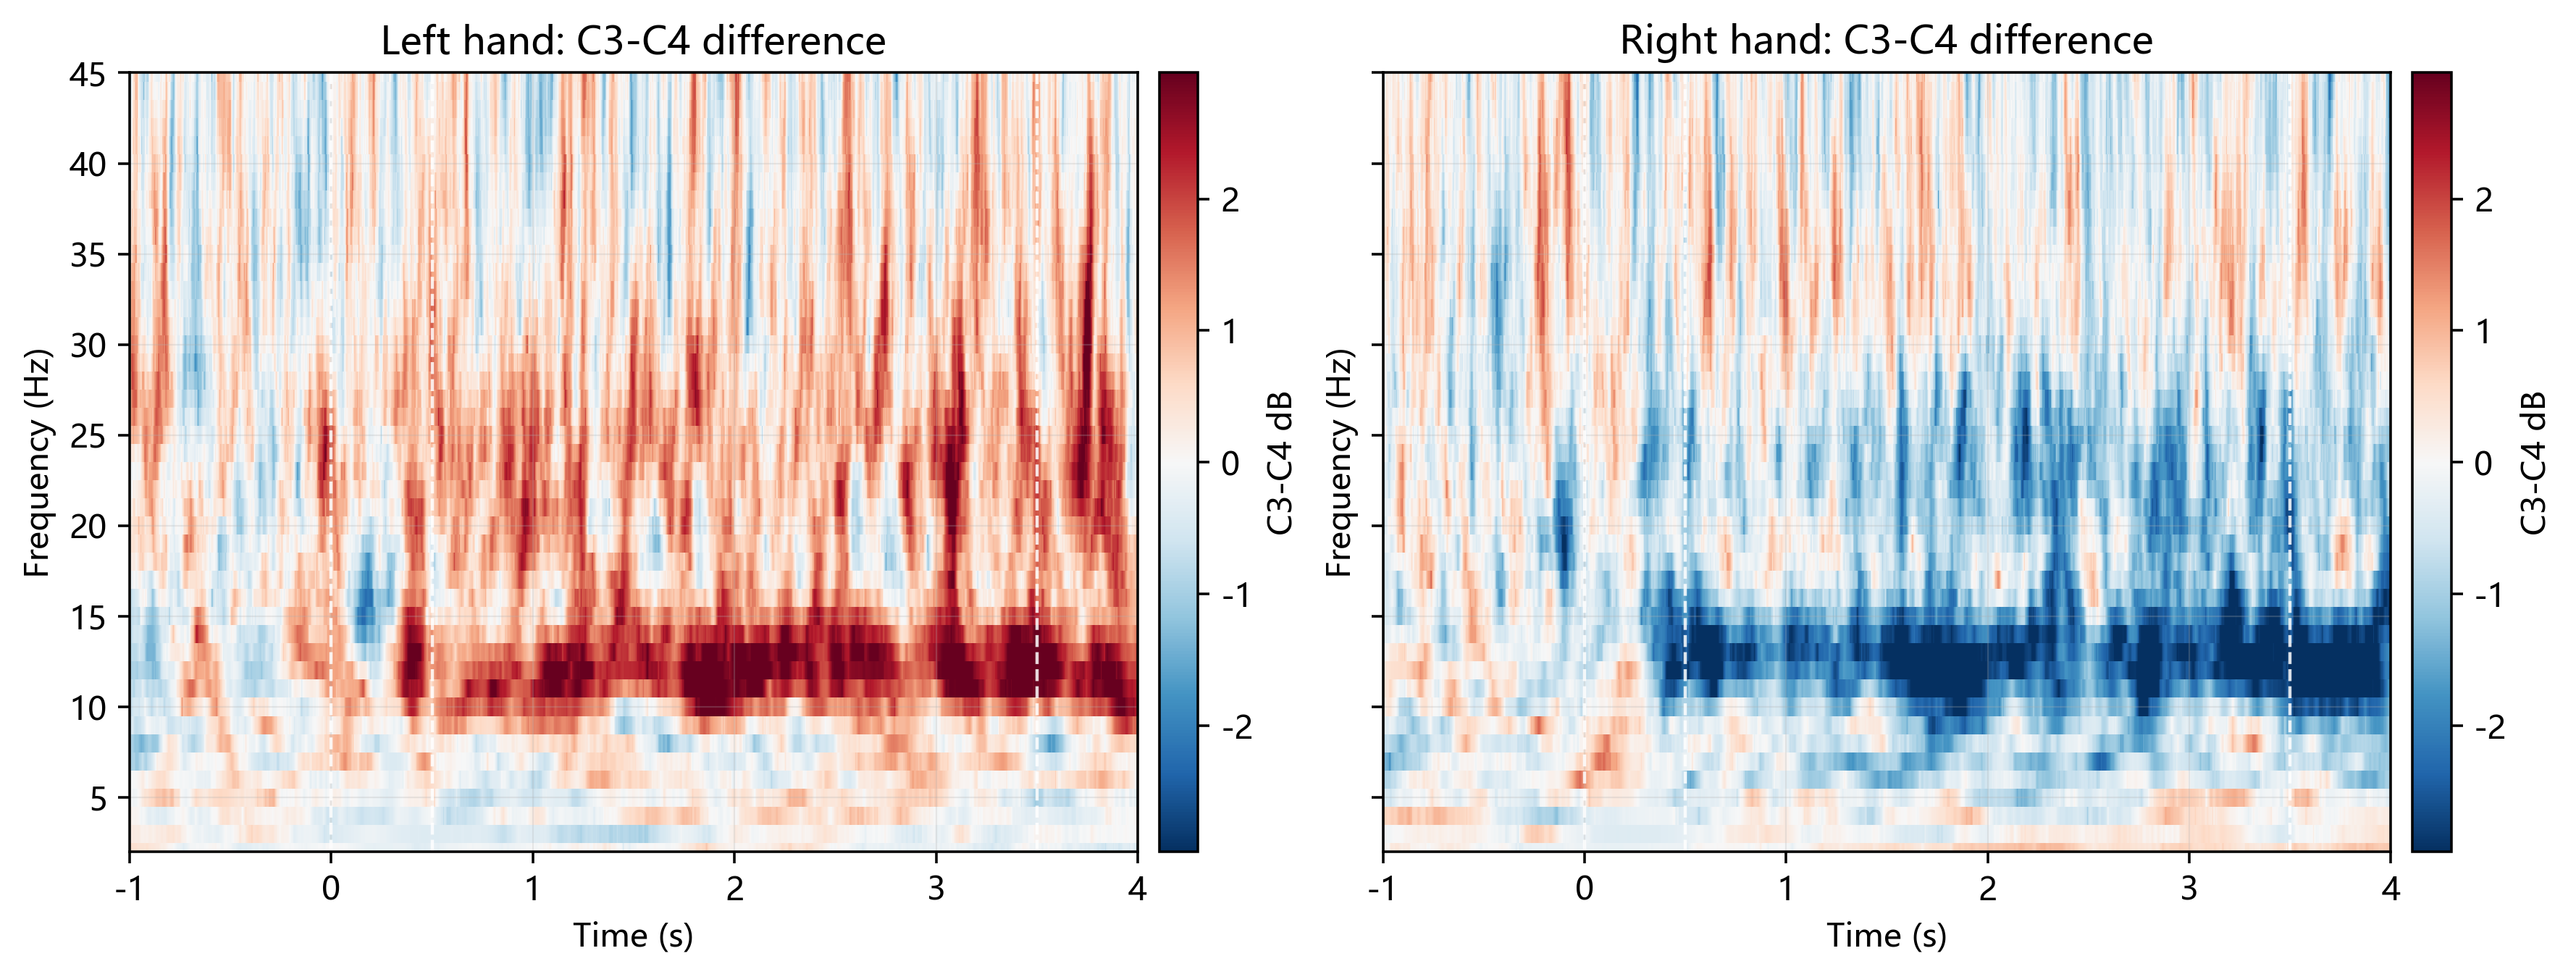
\includegraphics[width=0.96\textwidth]{exp4_c3_minus_c4_tfr.png}
\caption{C3-C4 difference maps. Because ERD is negative, sign interpretation must account for which channel decreases more strongly.}
\label{fig:exp4-diff}
\end{figure}


Figure \ref{fig:exp4-curves} averages mu and beta bands over frequency to show their temporal evolution. The shaded task window links the two-dimensional maps to the summary metrics.

\begin{figure}[H]
\centering
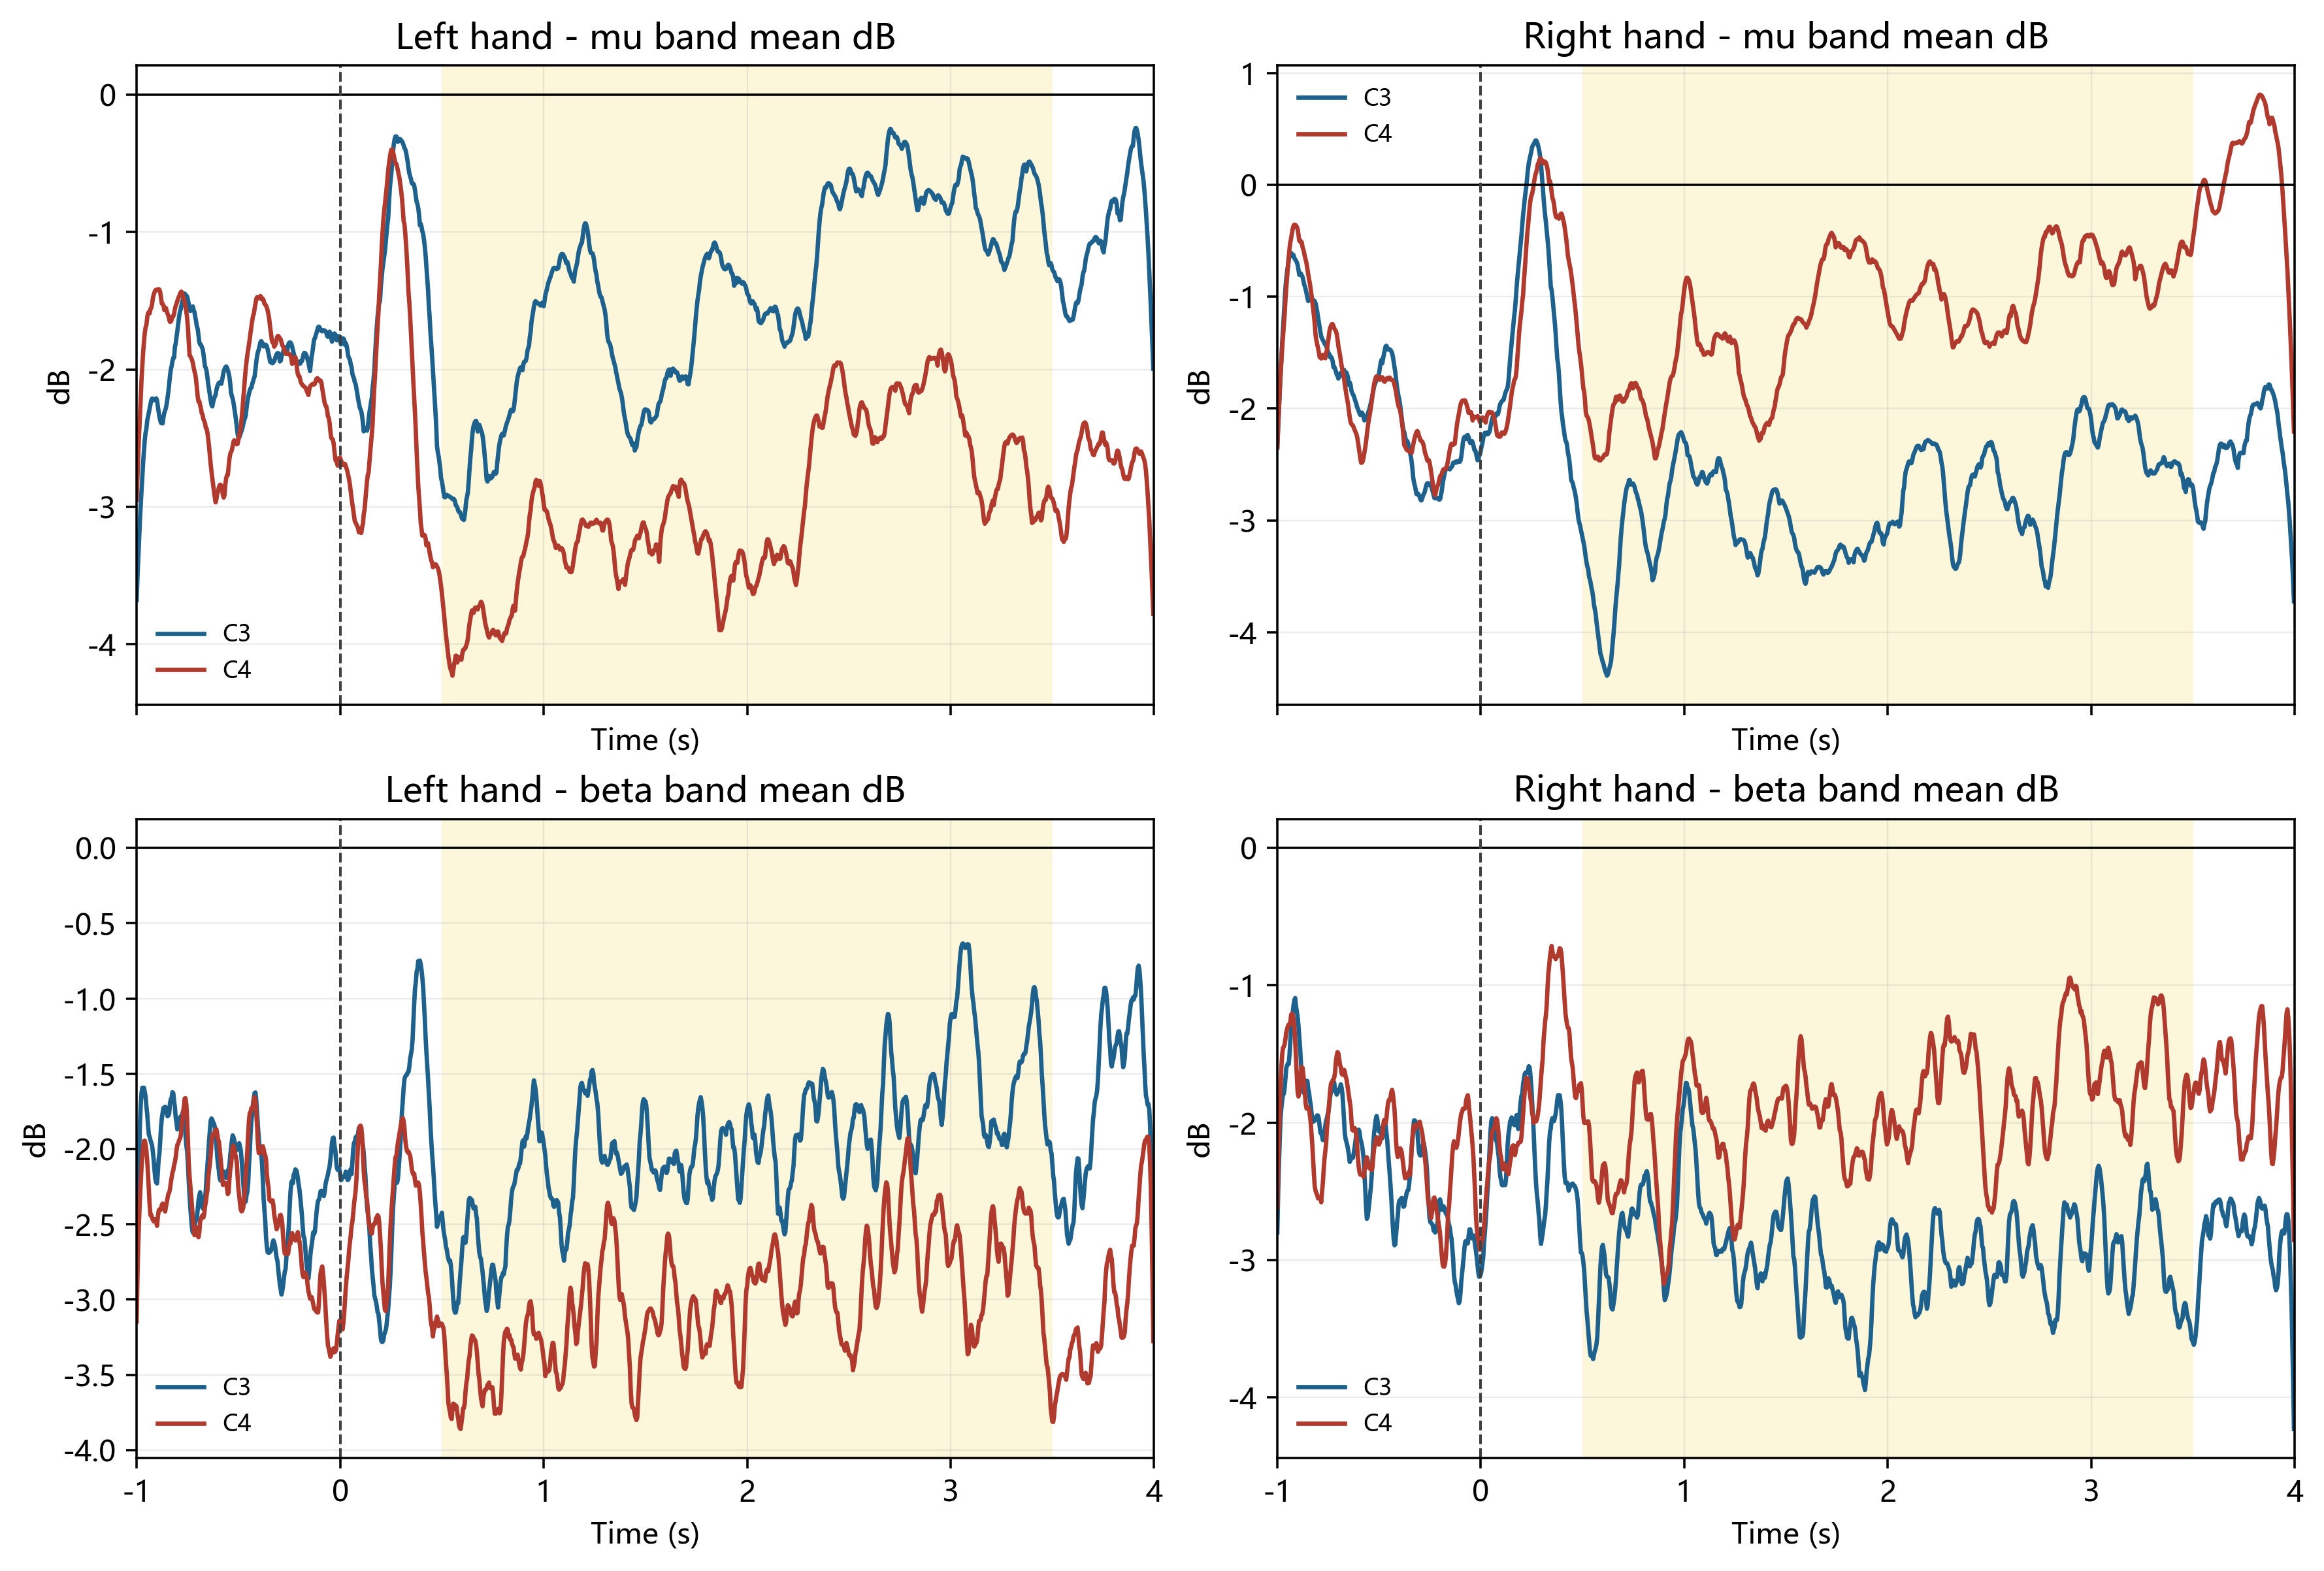
\includegraphics[width=0.96\textwidth]{exp4_mu_beta_time_curves.png}
\caption{Mu and beta band mean dB curves over time for C3 and C4.}
\label{fig:exp4-curves}
\end{figure}


Figure \ref{fig:exp4-bars} summarizes task-window means. A more negative bar indicates stronger ERD.

\begin{figure}[H]
\centering
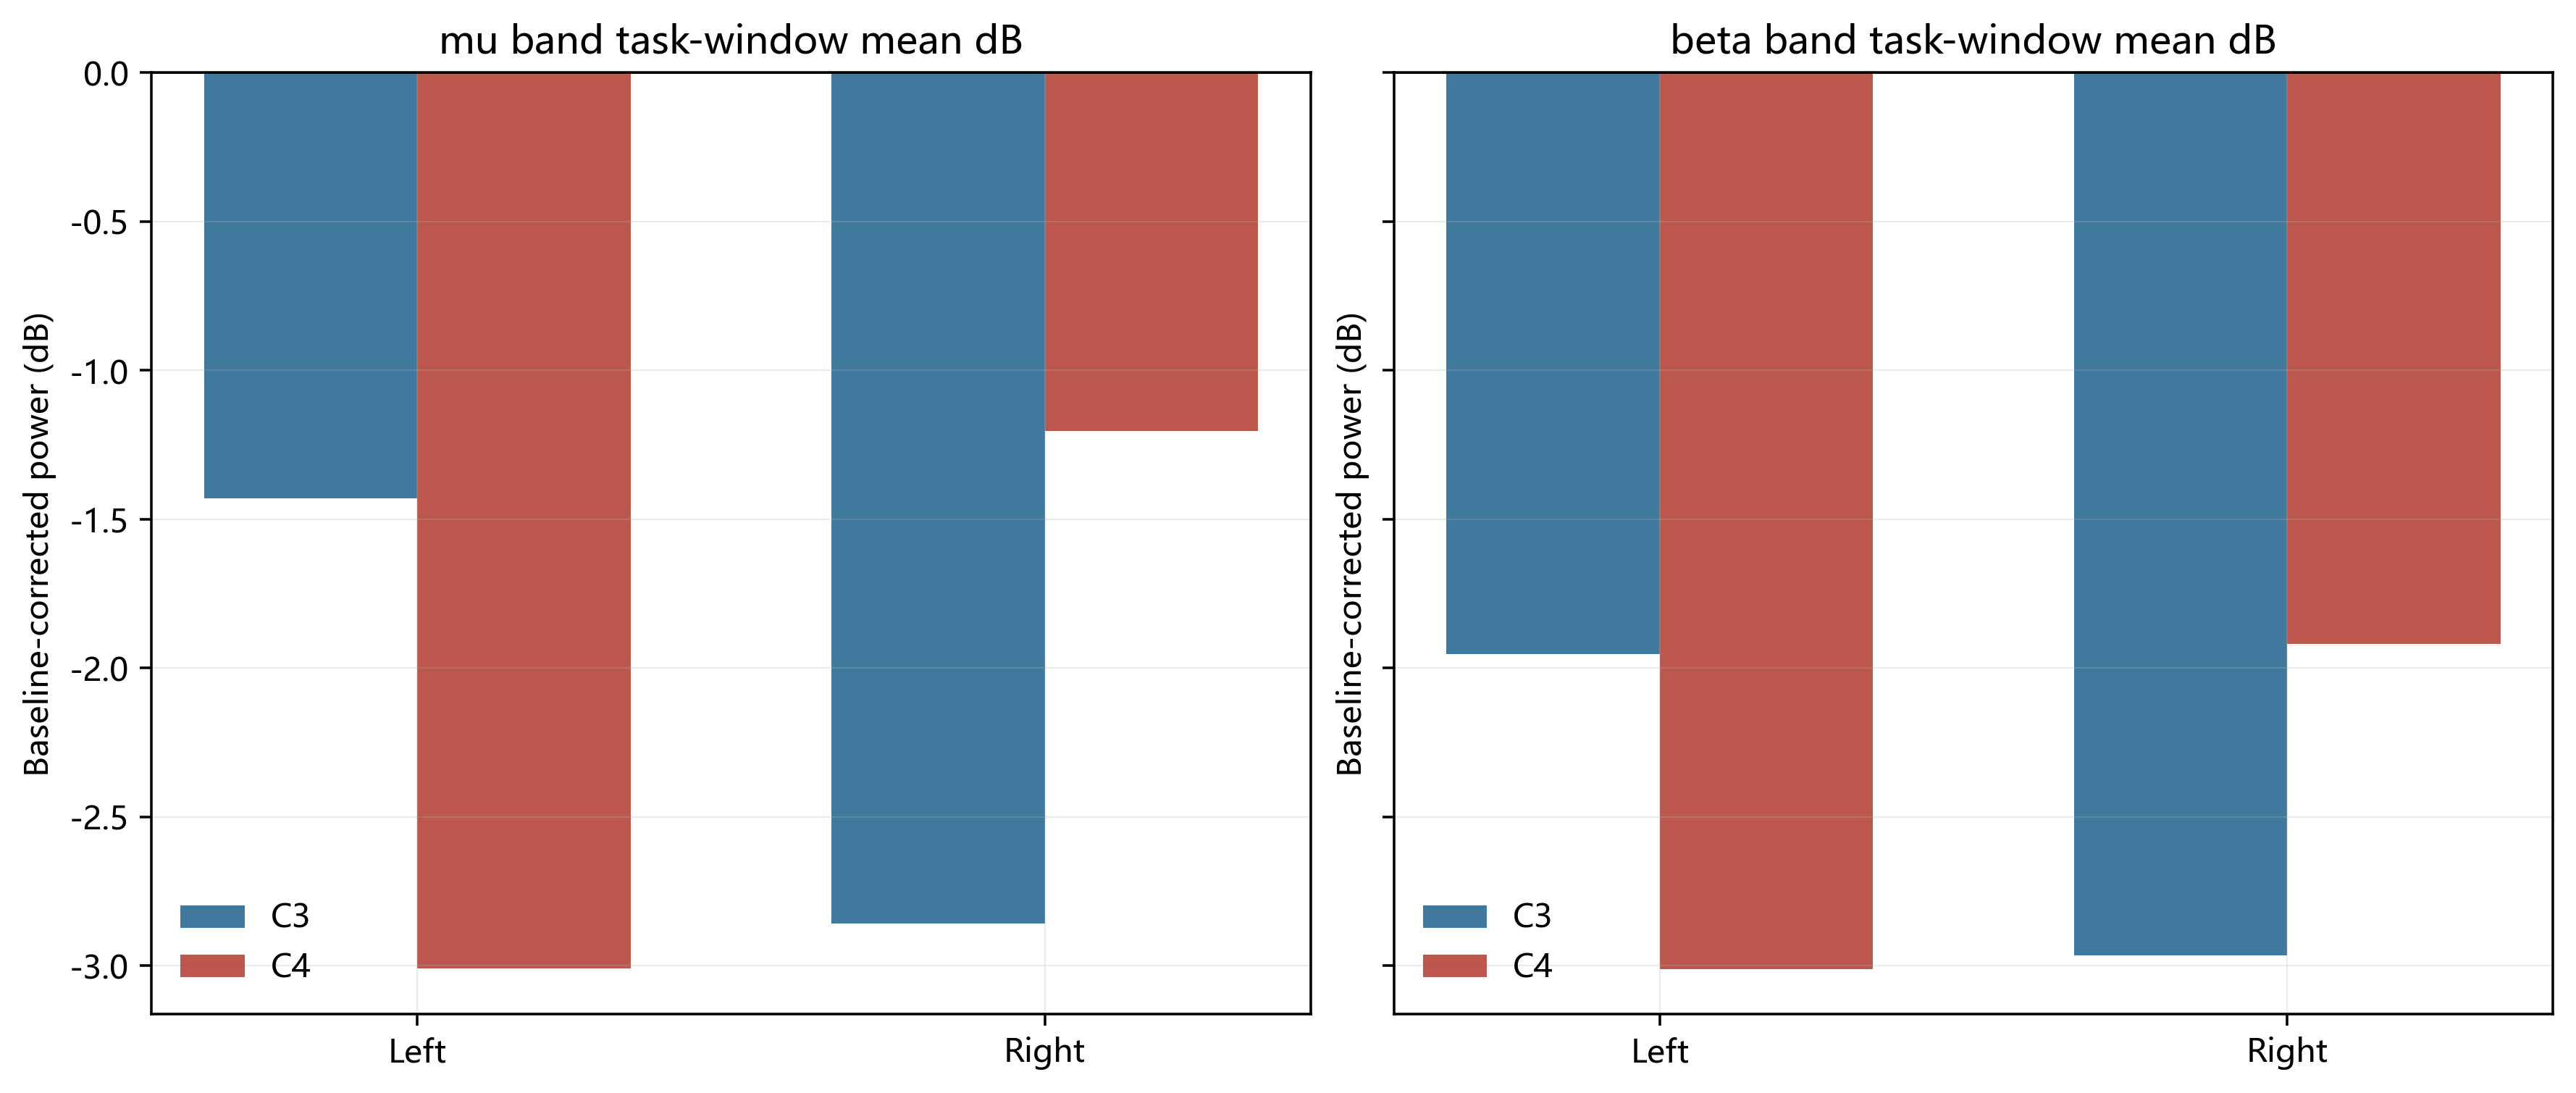
\includegraphics[width=0.90\textwidth]{exp4_band_mean_bars.png}
\caption{Task-window C3/C4 mean dB values in the mu and beta bands.}
\label{fig:exp4-bars}
\end{figure}


Figure \ref{fig:exp4-latfig} directly shows the lateralization metric. Left-hand mu and beta are positive, while right-hand mu and beta are negative, matching the expected contralateral pattern.

\begin{figure}[H]
\centering
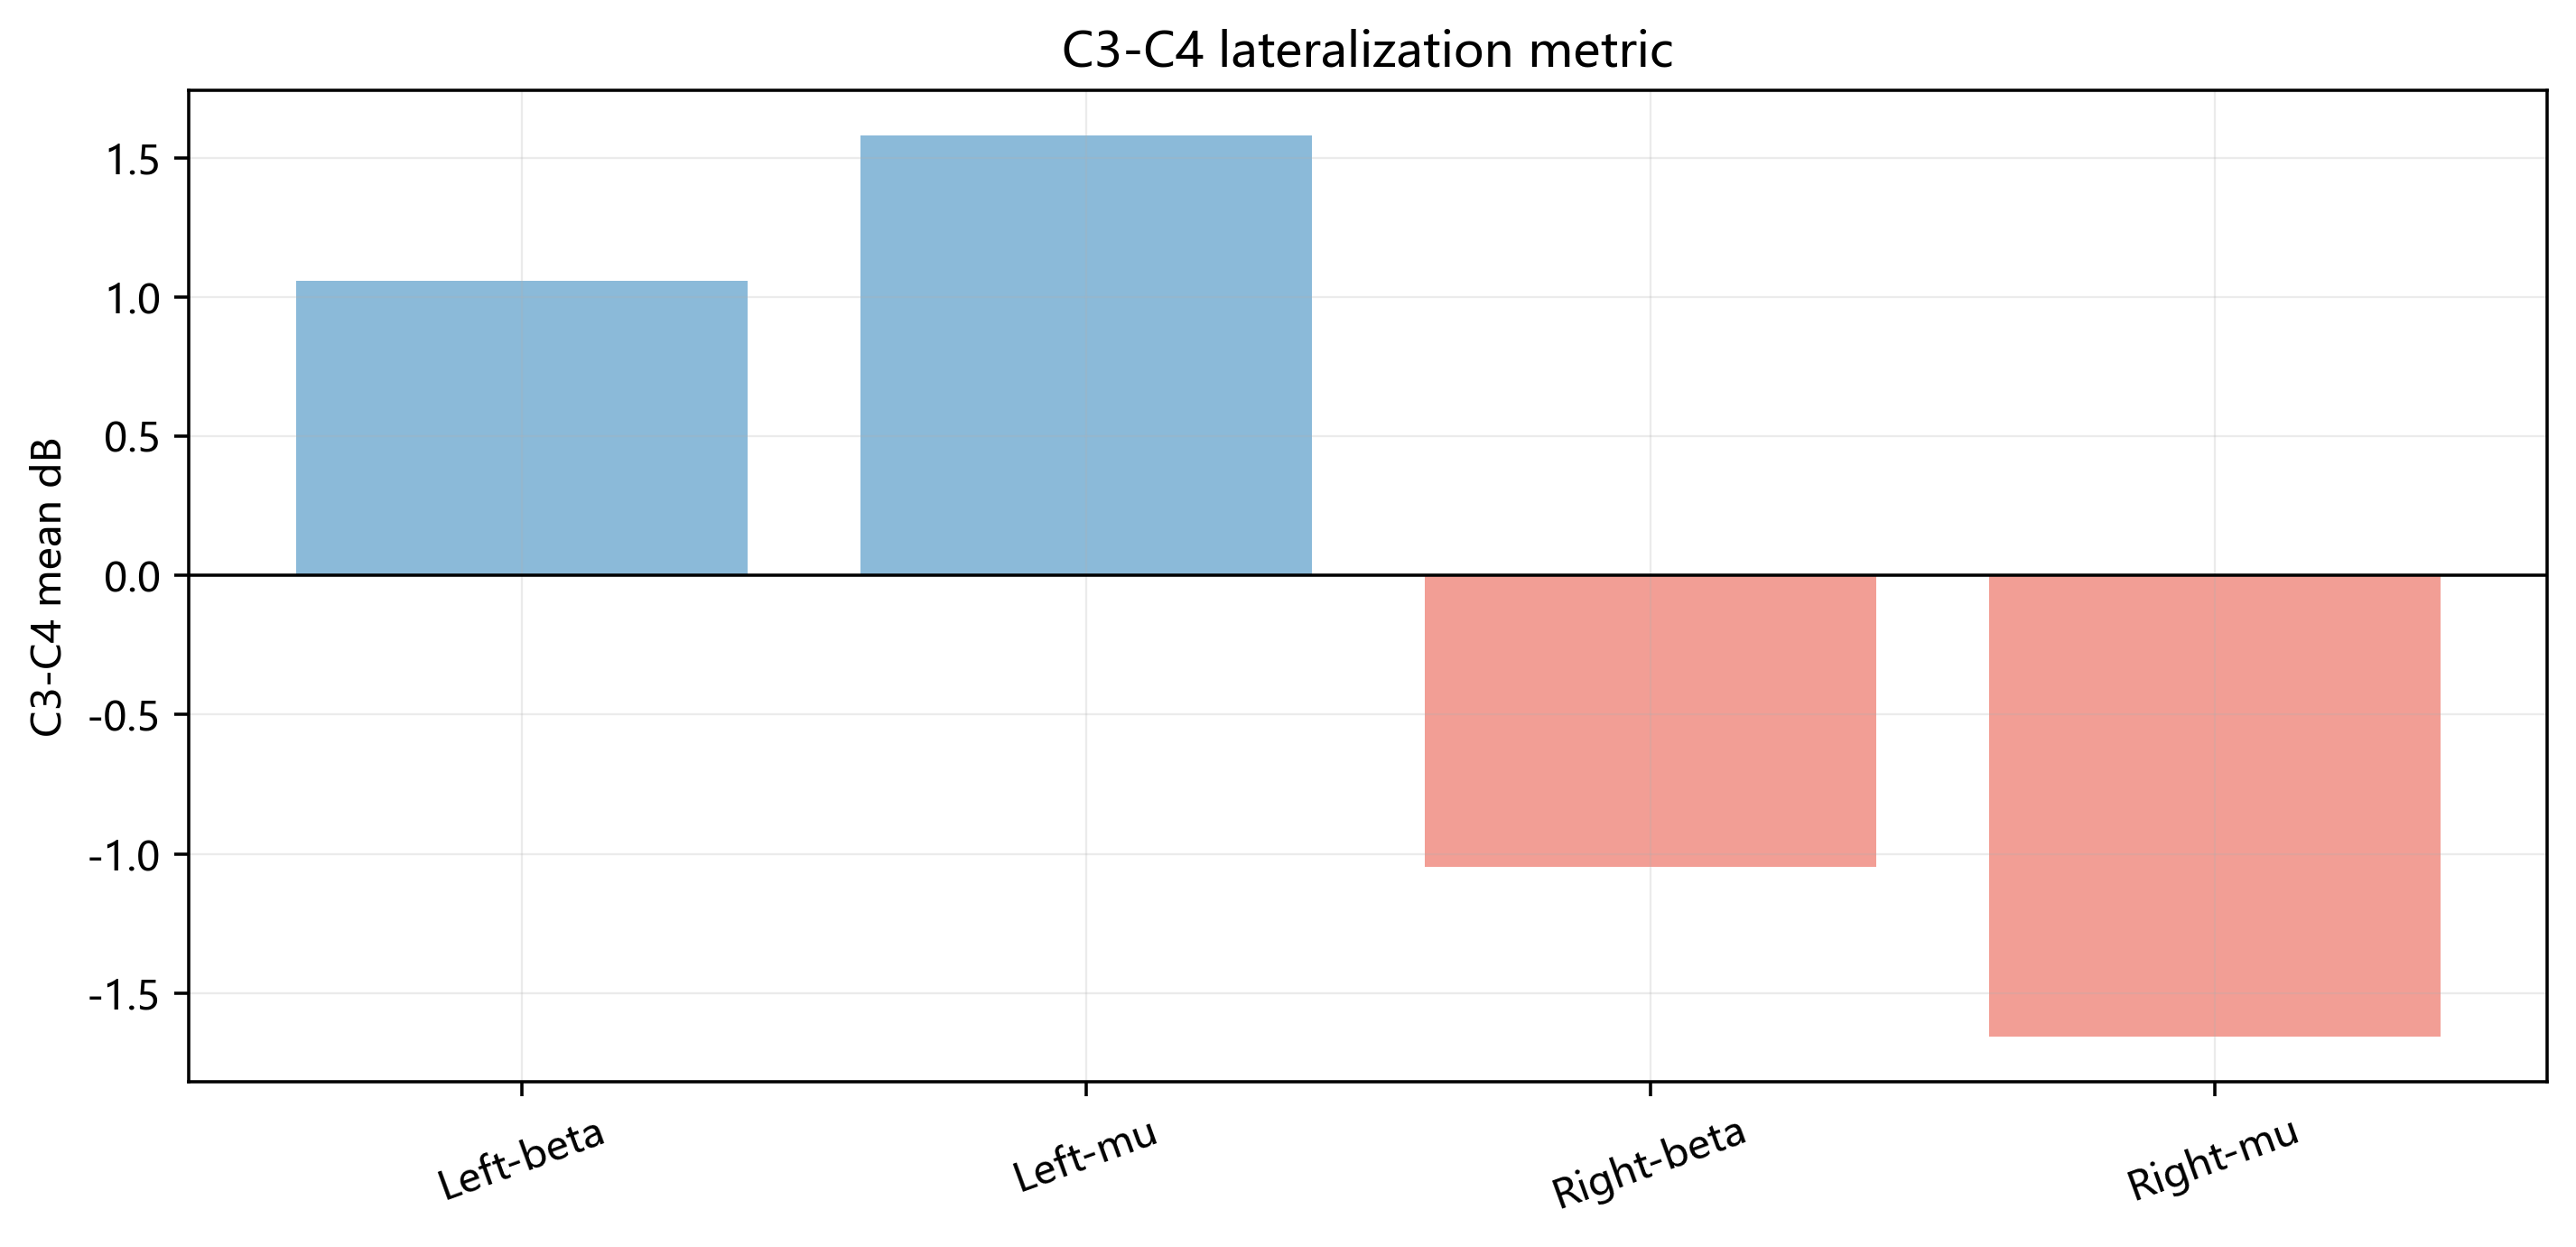
\includegraphics[width=0.82\textwidth]{exp4_lateralization_index.png}
\caption{C3-C4 lateralization metric. Left imagery is expected to be positive and right imagery negative when contralateral ERD dominates.}
\label{fig:exp4-latfig}
\end{figure}


Figure \ref{fig:exp4-neighbors} checks whether neighboring central channels support the C3/C4 interpretation. Neighboring channels help evaluate whether the effect is spatially plausible rather than an isolated channel fluctuation.

\begin{figure}[H]
\centering
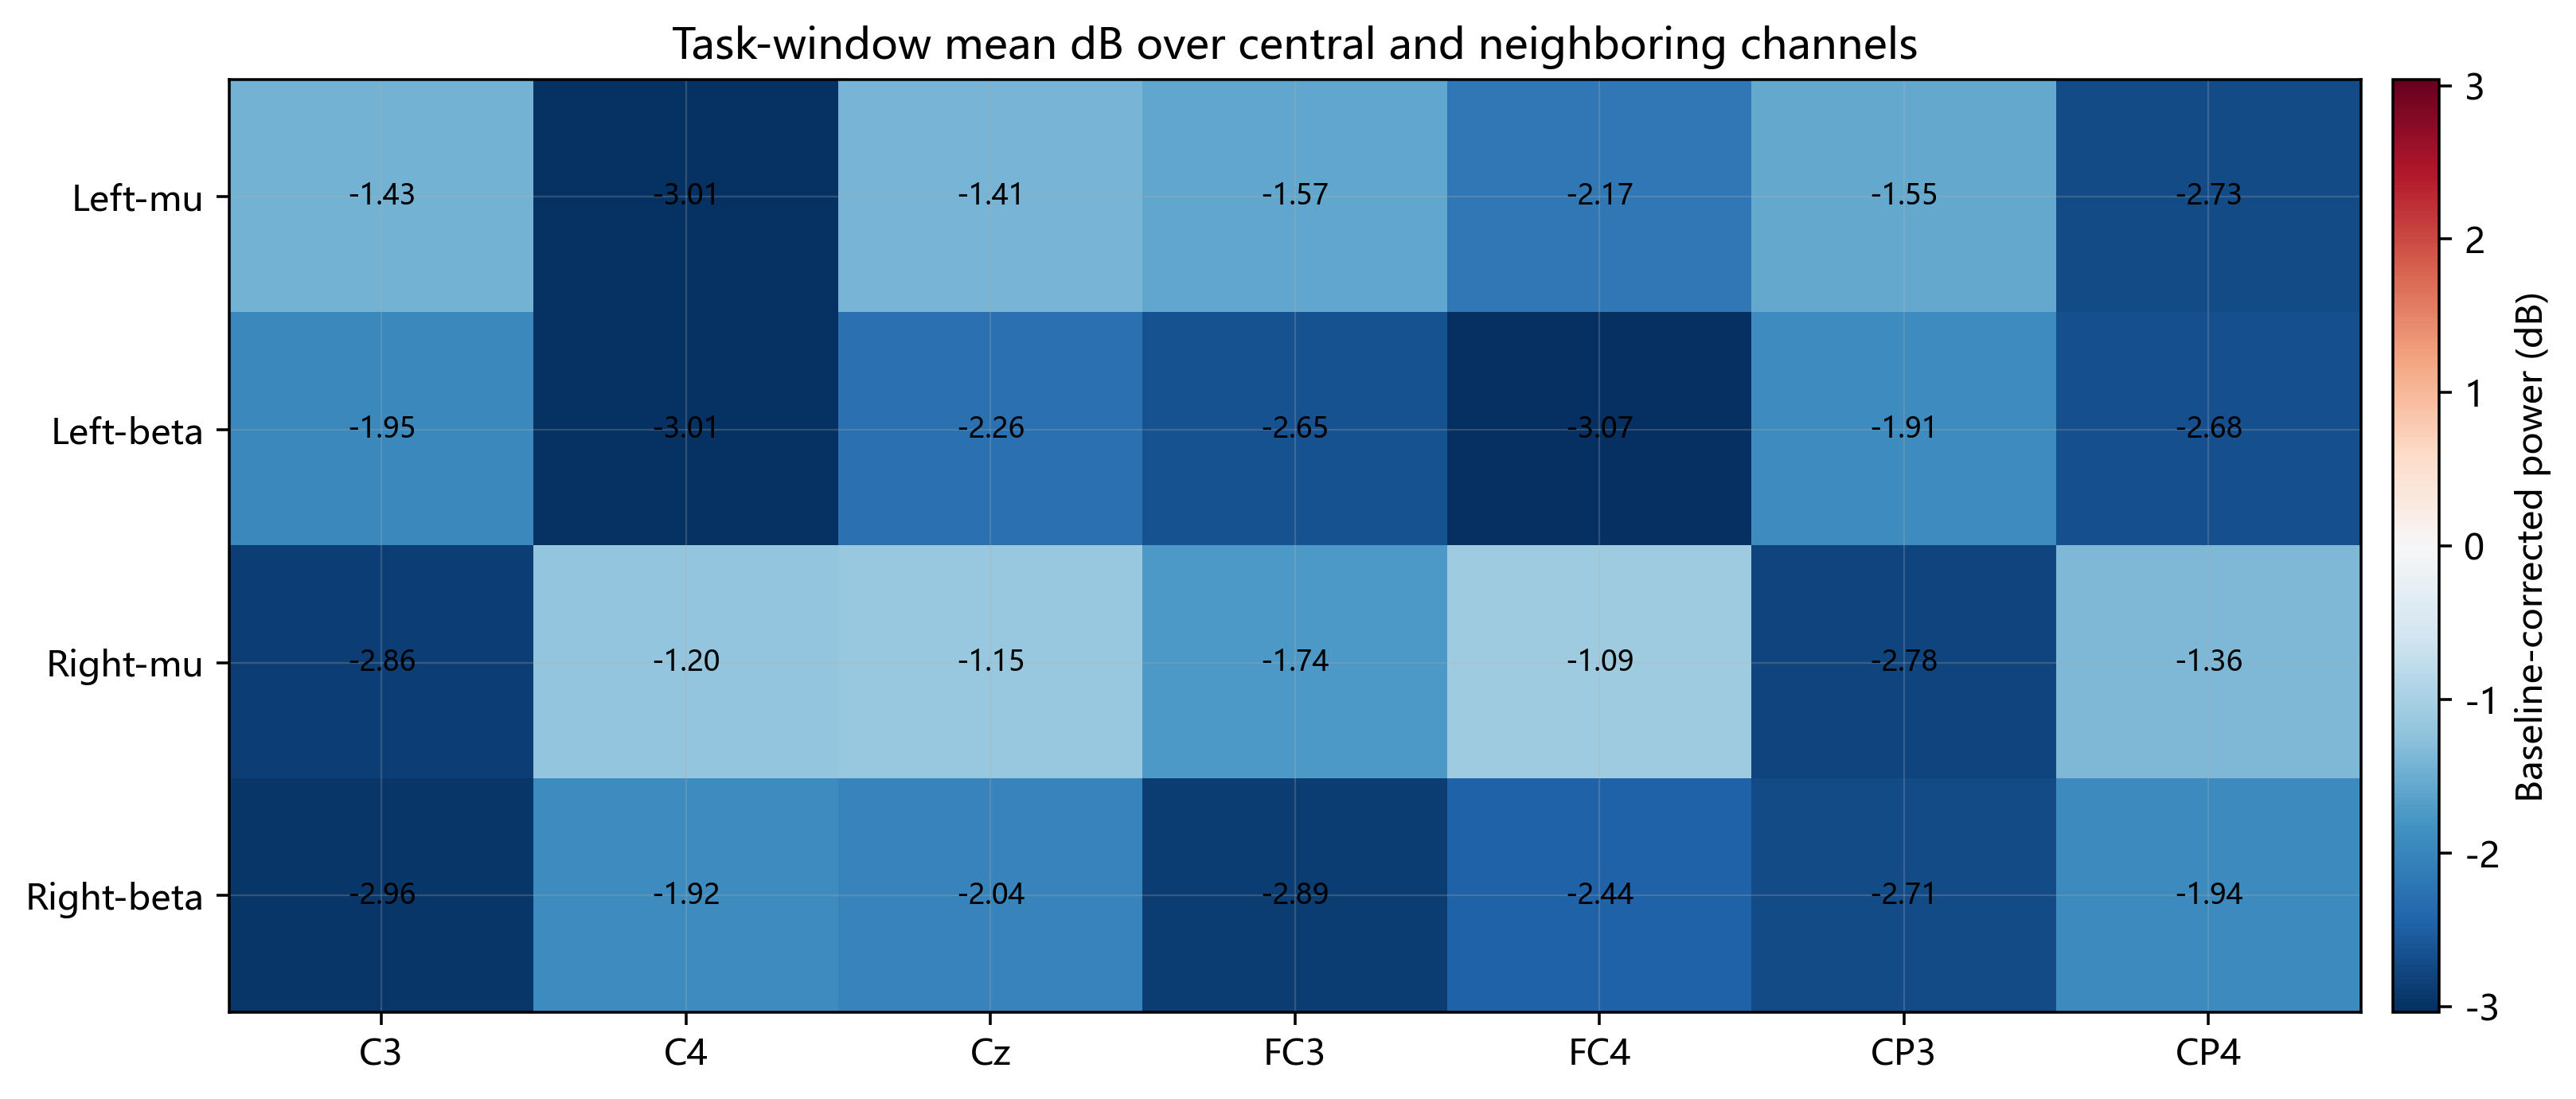
\includegraphics[width=0.90\textwidth]{exp4_neighbor_channel_heatmap.png}
\caption{Task-window mean dB across central and neighboring channels.}
\label{fig:exp4-neighbors}
\end{figure}


Figure \ref{fig:exp4-split} compares train and test splits. The split check is used as a robustness assessment for the combined analysis.

\begin{figure}[H]
\centering
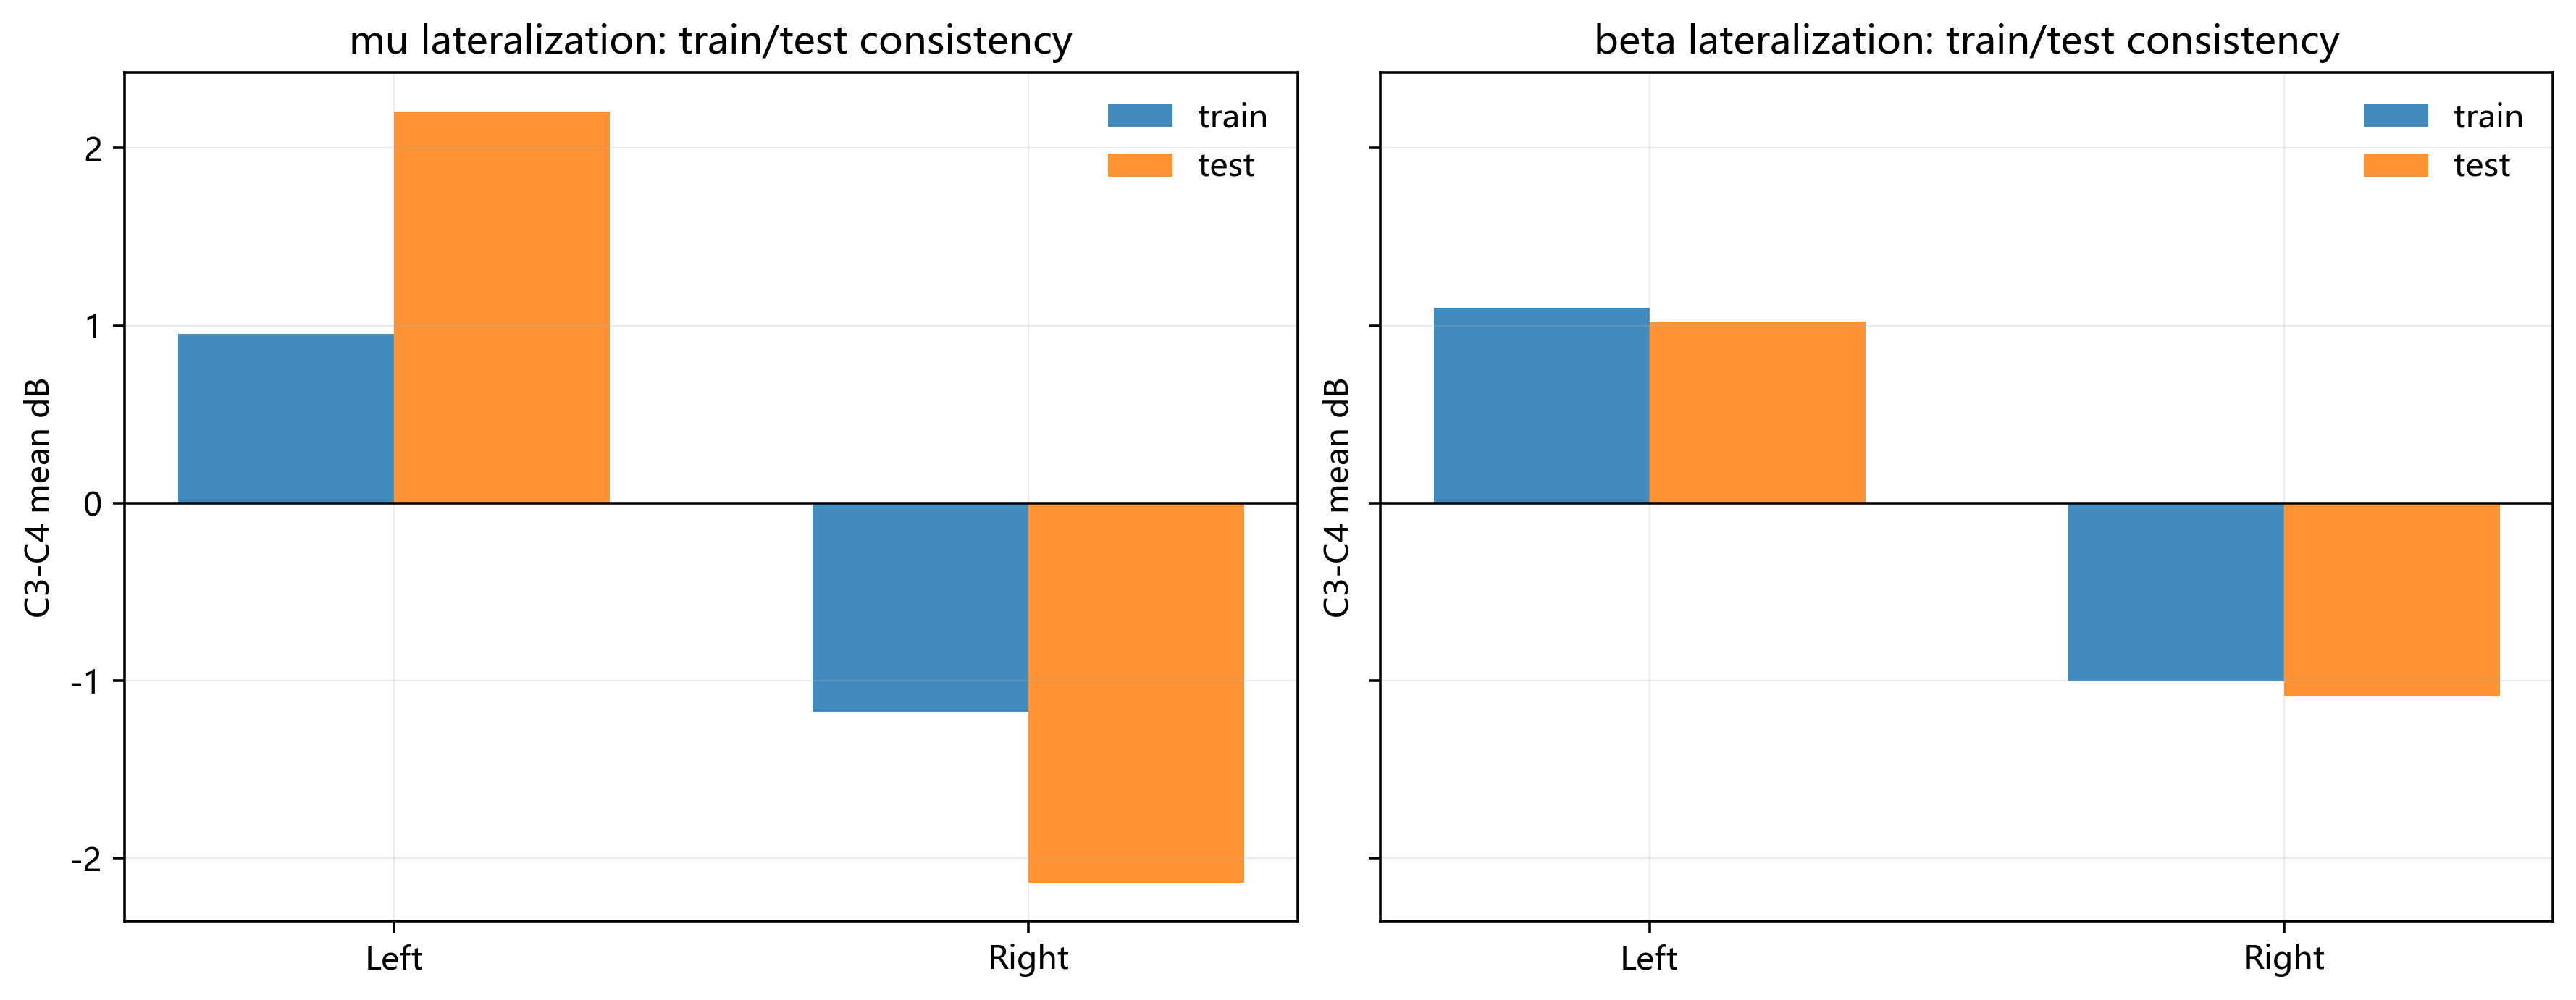
\includegraphics[width=0.90\textwidth]{exp4_train_test_consistency.png}
\caption{Train/test consistency of the C3-C4 lateralization metric.}
\label{fig:exp4-split}
\end{figure}


Tables \ref{tab:exp4-metrics} and \ref{tab:exp4-lat} provide numerical support. The left-hand condition has $L_\mu=1.580$ dB and $L_\beta=1.058$ dB; the right-hand condition has $L_\mu=-1.656$ dB and $L_\beta=-1.045$ dB.

\begin{table}[H]
\centering
\caption{Task-window mu/beta mean dB over central and neighboring channels.}
\label{tab:exp4-metrics}
\scriptsize
\resizebox{\textwidth}{!}{%
\begin{tabular}{llllll}
\toprule
Condition & Channel & Band & Mean dB & SD & Trials\\
\midrule
left & C3 & beta & -1.953 & 2.137 & 100.000\\
left & C4 & beta & -3.011 & 2.357 & 100.000\\
left & CP3 & beta & -1.915 & 2.031 & 100.000\\
left & CP4 & beta & -2.680 & 2.246 & 100.000\\
left & Cz & beta & -2.261 & 1.825 & 100.000\\
left & FC3 & beta & -2.649 & 1.911 & 100.000\\
left & FC4 & beta & -3.069 & 2.004 & 100.000\\
right & C3 & beta & -2.965 & 1.970 & 100.000\\
right & C4 & beta & -1.919 & 2.607 & 100.000\\
right & CP3 & beta & -2.714 & 1.858 & 100.000\\
right & CP4 & beta & -1.943 & 2.383 & 100.000\\
right & Cz & beta & -2.039 & 2.169 & 100.000\\
right & FC3 & beta & -2.892 & 1.799 & 100.000\\
right & FC4 & beta & -2.445 & 2.457 & 100.000\\
left & C3 & mu & -1.429 & 3.650 & 100.000\\
left & C4 & mu & -3.008 & 3.245 & 100.000\\
left & CP3 & mu & -1.550 & 3.517 & 100.000\\
left & CP4 & mu & -2.728 & 3.359 & 100.000\\
left & Cz & mu & -1.411 & 2.946 & 100.000\\
left & FC3 & mu & -1.571 & 3.102 & 100.000\\
left & FC4 & mu & -2.175 & 3.230 & 100.000\\
right & C3 & mu & -2.859 & 3.408 & 100.000\\
right & C4 & mu & -1.203 & 3.740 & 100.000\\
right & CP3 & mu & -2.785 & 3.422 & 100.000\\
right & CP4 & mu & -1.362 & 3.729 & 100.000\\
right & Cz & mu & -1.147 & 2.986 & 100.000\\
right & FC3 & mu & -1.736 & 2.868 & 100.000\\
right & FC4 & mu & -1.087 & 3.246 & 100.000\\
\bottomrule
\end{tabular}
}
\end{table}


\begin{table}[H]
\centering
\caption{C3-C4 lateralization metrics and expected interpretation.}
\label{tab:exp4-lat}
\scriptsize
\resizebox{\textwidth}{!}{%
\begin{tabular}{llllll}
\toprule
Condition & Band & C3 dB & C4 dB & C3-C4 & Expected direction\\
\midrule
left & beta & -1.953 & -3.011 & 1.058 & left imagery: stronger C4 ERD, C3-C4 positive\\
left & mu & -1.429 & -3.008 & 1.580 & left imagery: stronger C4 ERD, C3-C4 positive\\
right & beta & -2.965 & -1.919 & -1.045 & right imagery: stronger C3 ERD, C3-C4 negative\\
right & mu & -2.859 & -1.203 & -1.656 & right imagery: stronger C3 ERD, C3-C4 negative\\
\bottomrule
\end{tabular}
}
\end{table}


\subsection{Analysis and Discussion}
Figure \ref{fig:exp4-epoch} and Figure \ref{fig:exp4-pipeline} define the comparison before observing results. The baseline window is pre-cue and does not include the motor imagery task. Trial-wise CWT and baseline correction precede condition averaging; otherwise non-phase-locked rhythms could cancel if raw EEG waveforms were averaged first.

The main analysis focuses on 8--13 Hz mu and 13--30 Hz beta bands. Figure \ref{fig:exp4-tfr} shows baseline-corrected C3/C4 maps, Figure \ref{fig:exp4-curves} compresses bands into time curves, and Table \ref{tab:exp4-metrics} gives task-window means. Figure \ref{fig:exp4-bars} allows direct C3/C4 comparison; Figure \ref{fig:exp4-neighbors} examines spatial consistency; Figure \ref{fig:exp4-split} checks train/test robustness.

The lateralization direction is clear in this subject. Left imagery yields positive $L_\mu$ and $L_\beta$, consistent with stronger C4 ERD. Right imagery yields negative $L_\mu$ and $L_\beta$, consistent with stronger C3 ERD. The interpretation must account for ERD being a negative dB change: a positive difference does not mean more activation; it may mean that C4 decreased more strongly.

\paragraph{Question: Why are C3, C4, and Cz commonly used in motor imagery EEG instead of arbitrary channels?}
Answer: C3, C4, and Cz lie over central sensorimotor regions. Hand motor imagery modulates mu/beta rhythms near these areas, and left/right hand imagery often shows contralateral dominance. This report locates the channels by name and also examines FC3/FC4 and CP3/CP4 as neighboring support.

\paragraph{Question: Why is baseline correction needed for ERD, and what can go wrong with raw power maps?}
Answer: Absolute power differs by frequency, channel, electrode condition, and individual rhythm strength. Raw power maps may confuse these background differences with task effects. Baseline correction compares each frequency with its own pre-cue reference, making negative dB values interpretable as event-related power decreases.

\paragraph{Question: How can C3/C4 baseline-corrected maps be used to judge lateralization in left and right imagery?}
Answer: First check whether mu/beta ERD appears as negative dB in the task window. Then compare the contralateral channel. Left imagery is expected to show stronger C4 ERD; right imagery is expected to show stronger C3 ERD. The metric $L_b=C3-C4$ summarizes this sign pattern.

\paragraph{Question: What is the advantage of a C3-C4 difference map, and what can it hide?}
Answer: A difference map directly emphasizes relative left-right central changes. However, it hides absolute channel values. If both channels show strong ERD, their difference may be small. If one channel contains noise, the difference can be misleading. It should therefore be interpreted with single-channel maps, curves, and tables.

\paragraph{Question: If one subject's ERD is weak, what physiological or analytical factors may explain it?}
Answer: Physiological factors include weak sensorimotor rhythm, inconsistent imagery strategy, attention fluctuation, fatigue, and individual BCI variability. Analytical factors include baseline choice, task-window choice, channel position, filtering, time-frequency parameters, noise, and artifacts. Weak ERD does not automatically imply a processing error.

\FloatBarrier
\clearpage
\section{Conclusion}
The four experiments show that time-frequency maps are evidence produced by a signal, an analysis model, and parameter choices. The full Fourier spectrum summarizes global frequency content but cannot express occurrence time. STFT provides local spectra through sliding windows, but its window length and window function determine the time-frequency tradeoff. CWT distributes resolution across scales and is useful for signals containing sustained low frequencies and transient high frequencies. In real motor imagery EEG, baseline correction, trial-wise power averaging, and C3/C4 plus neighboring-channel comparisons are essential for interpreting ERD and lateralization.

\appendix
\clearpage
\section{Appendix A: Supplementary Outputs and Data Dictionary}
The project outputs include PNG figures in \texttt{results/figures} and \texttt{results\_en/figures}, CSV metric tables in \texttt{results/tables}, JSON/trajectory data in \texttt{results/data}, and an EEG time-frequency average cache in \texttt{results/cache}. The EEG cache stores \texttt{avg\_all}, \texttt{avg\_train}, and \texttt{avg\_test} arrays with dimensions condition, channel, frequency, and time.

\section{Appendix B: Core Code Snippets}
\subsection{STFT, CWT, and Multiresolution Utility Functions}
\lstinputlisting[firstline=32,lastline=179]{../scripts/signal_utils.py}

\subsection{Core Trial-wise EEG Time-Frequency Averaging}
\lstinputlisting[firstline=124,lastline=167]{../scripts/experiment4_eeg.py}

\section{Appendix C: Reproduction Commands}
\begin{lstlisting}[language=bash]
uv venv --python 3.12 .venv
uv pip install -r requirements.txt
.venv\Scripts\python scripts\run_all_public.py
.venv\Scripts\python scripts\english_figures.py
.venv\Scripts\python scripts\report_writer_en.py
.venv\Scripts\python scripts\build_report_en.py
\end{lstlisting}

\end{document}
